% Options for packages loaded elsewhere
\PassOptionsToPackage{unicode}{hyperref}
\PassOptionsToPackage{hyphens}{url}
\PassOptionsToPackage{dvipsnames,svgnames,x11names}{xcolor}
%
\documentclass[
  a4paper,
  DIV=11,
  numbers=noendperiod,
  oneside,
  open=any]{scrreport}

\usepackage{amsmath,amssymb}
\usepackage{iftex}
\ifPDFTeX
  \usepackage[T1]{fontenc}
  \usepackage[utf8]{inputenc}
  \usepackage{textcomp} % provide euro and other symbols
\else % if luatex or xetex
  \usepackage{unicode-math}
  \defaultfontfeatures{Scale=MatchLowercase}
  \defaultfontfeatures[\rmfamily]{Ligatures=TeX,Scale=1}
\fi
\usepackage{lmodern}
\ifPDFTeX\else  
    % xetex/luatex font selection
\fi
% Use upquote if available, for straight quotes in verbatim environments
\IfFileExists{upquote.sty}{\usepackage{upquote}}{}
\IfFileExists{microtype.sty}{% use microtype if available
  \usepackage[]{microtype}
  \UseMicrotypeSet[protrusion]{basicmath} % disable protrusion for tt fonts
}{}
\makeatletter
\@ifundefined{KOMAClassName}{% if non-KOMA class
  \IfFileExists{parskip.sty}{%
    \usepackage{parskip}
  }{% else
    \setlength{\parindent}{0pt}
    \setlength{\parskip}{6pt plus 2pt minus 1pt}}
}{% if KOMA class
  \KOMAoptions{parskip=half}}
\makeatother
\usepackage{xcolor}
\setlength{\emergencystretch}{3em} % prevent overfull lines
\setcounter{secnumdepth}{5}
% Make \paragraph and \subparagraph free-standing
\ifx\paragraph\undefined\else
  \let\oldparagraph\paragraph
  \renewcommand{\paragraph}[1]{\oldparagraph{#1}\mbox{}}
\fi
\ifx\subparagraph\undefined\else
  \let\oldsubparagraph\subparagraph
  \renewcommand{\subparagraph}[1]{\oldsubparagraph{#1}\mbox{}}
\fi


\providecommand{\tightlist}{%
  \setlength{\itemsep}{0pt}\setlength{\parskip}{0pt}}\usepackage{longtable,booktabs,array}
\usepackage{calc} % for calculating minipage widths
% Correct order of tables after \paragraph or \subparagraph
\usepackage{etoolbox}
\makeatletter
\patchcmd\longtable{\par}{\if@noskipsec\mbox{}\fi\par}{}{}
\makeatother
% Allow footnotes in longtable head/foot
\IfFileExists{footnotehyper.sty}{\usepackage{footnotehyper}}{\usepackage{footnote}}
\makesavenoteenv{longtable}
\usepackage{graphicx}
\makeatletter
\def\maxwidth{\ifdim\Gin@nat@width>\linewidth\linewidth\else\Gin@nat@width\fi}
\def\maxheight{\ifdim\Gin@nat@height>\textheight\textheight\else\Gin@nat@height\fi}
\makeatother
% Scale images if necessary, so that they will not overflow the page
% margins by default, and it is still possible to overwrite the defaults
% using explicit options in \includegraphics[width, height, ...]{}
\setkeys{Gin}{width=\maxwidth,height=\maxheight,keepaspectratio}
% Set default figure placement to htbp
\makeatletter
\def\fps@figure{htbp}
\makeatother

\usepackage[noblocks]{authblk}
\renewcommand*{\Authsep}{, }
\renewcommand*{\Authand}{, }
\renewcommand*{\Authands}{, }
\renewcommand\Affilfont{\small}
\KOMAoption{captions}{tableheading}
\usepackage{fancyhdr}
\usepackage{xcolor}
\usepackage{iftex}
\usepackage[english]{babel}
\pagestyle{fancy}
\fancyhead[RO, RE]{\url{https://github.com/JD2112/methylr}}
\fancyfoot[RO, RE]{\color{violet} \textcopyright Volpe, M \& Das, J}
\makeatletter
\@ifpackageloaded{tcolorbox}{}{\usepackage[skins,breakable]{tcolorbox}}
\@ifpackageloaded{fontawesome5}{}{\usepackage{fontawesome5}}
\definecolor{quarto-callout-color}{HTML}{909090}
\definecolor{quarto-callout-note-color}{HTML}{0758E5}
\definecolor{quarto-callout-important-color}{HTML}{CC1914}
\definecolor{quarto-callout-warning-color}{HTML}{EB9113}
\definecolor{quarto-callout-tip-color}{HTML}{00A047}
\definecolor{quarto-callout-caution-color}{HTML}{FC5300}
\definecolor{quarto-callout-color-frame}{HTML}{acacac}
\definecolor{quarto-callout-note-color-frame}{HTML}{4582ec}
\definecolor{quarto-callout-important-color-frame}{HTML}{d9534f}
\definecolor{quarto-callout-warning-color-frame}{HTML}{f0ad4e}
\definecolor{quarto-callout-tip-color-frame}{HTML}{02b875}
\definecolor{quarto-callout-caution-color-frame}{HTML}{fd7e14}
\makeatother
\makeatletter
\@ifpackageloaded{bookmark}{}{\usepackage{bookmark}}
\makeatother
\makeatletter
\@ifpackageloaded{caption}{}{\usepackage{caption}}
\AtBeginDocument{%
\ifdefined\contentsname
  \renewcommand*\contentsname{Table of contents}
\else
  \newcommand\contentsname{Table of contents}
\fi
\ifdefined\listfigurename
  \renewcommand*\listfigurename{List of Figures}
\else
  \newcommand\listfigurename{List of Figures}
\fi
\ifdefined\listtablename
  \renewcommand*\listtablename{List of Tables}
\else
  \newcommand\listtablename{List of Tables}
\fi
\ifdefined\figurename
  \renewcommand*\figurename{Figure}
\else
  \newcommand\figurename{Figure}
\fi
\ifdefined\tablename
  \renewcommand*\tablename{Table}
\else
  \newcommand\tablename{Table}
\fi
}
\@ifpackageloaded{float}{}{\usepackage{float}}
\floatstyle{ruled}
\@ifundefined{c@chapter}{\newfloat{codelisting}{h}{lop}}{\newfloat{codelisting}{h}{lop}[chapter]}
\floatname{codelisting}{Listing}
\newcommand*\listoflistings{\listof{codelisting}{List of Listings}}
\makeatother
\makeatletter
\makeatother
\makeatletter
\@ifpackageloaded{caption}{}{\usepackage{caption}}
\@ifpackageloaded{subcaption}{}{\usepackage{subcaption}}
\makeatother
\ifLuaTeX
  \usepackage{selnolig}  % disable illegal ligatures
\fi
\usepackage[citestyle = authoryear]{biblatex}
\addbibresource{references.bib}
\usepackage{bookmark}

\IfFileExists{xurl.sty}{\usepackage{xurl}}{} % add URL line breaks if available
\urlstyle{same} % disable monospaced font for URLs
\hypersetup{
  pdftitle={TranscriptR manual},
  pdfauthor={Massimiliano Volpe; Jyotirmoy Das},
  colorlinks=true,
  linkcolor={blue},
  filecolor={Maroon},
  citecolor={Blue},
  urlcolor={Blue},
  pdfcreator={LaTeX via pandoc}}

\title{TranscriptR manual}
\usepackage{etoolbox}
\makeatletter
\providecommand{\subtitle}[1]{% add subtitle to \maketitle
  \apptocmd{\@title}{\par {\large #1 \par}}{}{}
}
\makeatother
\subtitle{Reproducible RNA-seq data analysis using TranscriptR}
\author{Massimiliano Volpe \and Jyotirmoy Das}
\date{}

\begin{document}
\maketitle

\renewcommand*\contentsname{Contents}
{
\hypersetup{linkcolor=blue}
\setcounter{tocdepth}{1}
\tableofcontents
}
\listoffigures
\bookmarksetup{startatroot}

\chapter*{Acknowledgements}\label{acknowledgements}
\addcontentsline{toc}{chapter}{Acknowledgements}

\markboth{Acknowledgements}{Acknowledgements}

e-mail: \url{TranscriptR@googlegroups.com}

Bioinformatics,\\
Core Facility,\\
Faculty of Medicine and Health Sciences,\\
Linköping University,\\
Linköping,\\
Sweden

\textbf{\emph{We would like to acknowledge the Core Facility, Faculty of
Medicine and Health Sciences, Linköping University, Linköping, Sweden
and Clinical Genomics Linköping, Science for Life Laboratory, Sweden for
their support.}}

\bookmarksetup{startatroot}

\chapter*{Disclaimer}\label{disclaimer}
\addcontentsline{toc}{chapter}{Disclaimer}

\markboth{Disclaimer}{Disclaimer}

\textbf{\emph{All packages used in }TranscriptR* are publicly available
and open-source license. We have modified the source as required for
\emph{TranscriptR}. IGV genome viewer is inspired by
\href{https://github.com/gladkia/igvShiny}{igvShiny} Venn and UpSet
plots inspired by the
\href{https://github.com/asntech/intervene}{intervene} package
\autocite{khan2017intervene}, we modified as required for
\emph{TranscriptR}.}*

\begin{tcolorbox}[enhanced jigsaw, coltitle=black, colback=white, title=\textcolor{quarto-callout-important-color}{\faExclamation}\hspace{0.5em}{IMPORTANT}, leftrule=.75mm, titlerule=0mm, colframe=quarto-callout-important-color-frame, toprule=.15mm, opacityback=0, arc=.35mm, breakable, rightrule=.15mm, colbacktitle=quarto-callout-important-color!10!white, bottomtitle=1mm, opacitybacktitle=0.6, left=2mm, bottomrule=.15mm, toptitle=1mm]

\textbf{PLEASE NOTE} WE INCLUDED THE POSSIBILITY OF THE HUMAN
TRANSCRIPTOME DATA ANALYSIS FROM THE SEQUENCE DATA. NONE OF THE OWNER OF
THE CODE OR DATA CENTER IS RESPONSIBLE FOR HANDLING THE HUMAN DATA. IT
IS UPTO THE USER IF THEY WANT TO USE THE ONLINE VERSION FOR HUMAN DATA
ANALYSIS.

\end{tcolorbox}

\part{TranscriptR: Transcriptome Data Analysis Pipeline}

\begin{tcolorbox}[enhanced jigsaw, coltitle=black, colback=white, title=\textcolor{quarto-callout-important-color}{\faExclamation}\hspace{0.5em}{IMPORTANT}, leftrule=.75mm, titlerule=0mm, colframe=quarto-callout-important-color-frame, toprule=.15mm, opacityback=0, arc=.35mm, breakable, rightrule=.15mm, colbacktitle=quarto-callout-important-color!10!white, bottomtitle=1mm, opacitybacktitle=0.6, left=2mm, bottomrule=.15mm, toptitle=1mm]

PLEASE NOTE WE INCLUDED THE POSSIBILITY OF THE HUMAN TRANSCRIPTOME DATA
ANALYSIS FROM THE SEQUENCE DATA. NONE OF THE OWNER OF THE CODE OR DATA
CENTER IS RESPONSIBLE FOR HANDLING THE HUMAN DATA. IT IS UPTO THE USER
IF THEY WANT TO USE THE ONLINE VERSION FOR HUMAN DATA ANALYSIS.

\end{tcolorbox}

\begin{tcolorbox}[enhanced jigsaw, coltitle=black, colback=white, title=\textcolor{quarto-callout-warning-color}{\faExclamationTriangle}\hspace{0.5em}{Warning}, leftrule=.75mm, titlerule=0mm, colframe=quarto-callout-warning-color-frame, toprule=.15mm, opacityback=0, arc=.35mm, breakable, rightrule=.15mm, colbacktitle=quarto-callout-warning-color!10!white, bottomtitle=1mm, opacitybacktitle=0.6, left=2mm, bottomrule=.15mm, toptitle=1mm]

TO ALL OUR USERS, IF YOU ARE EXPERIENCING ANY TROUBLE WITH THE APP,
BEFORE SENDING THE BUG REPORT, PLEASE RESTART THE DOCKER CONTAINER AND
TRY AGAIN.

\end{tcolorbox}

\begin{tcolorbox}[enhanced jigsaw, coltitle=black, colback=white, title=\textcolor{quarto-callout-tip-color}{\faLightbulb}\hspace{0.5em}{Tip}, leftrule=.75mm, titlerule=0mm, colframe=quarto-callout-tip-color-frame, toprule=.15mm, opacityback=0, arc=.35mm, breakable, rightrule=.15mm, colbacktitle=quarto-callout-tip-color!10!white, bottomtitle=1mm, opacitybacktitle=0.6, left=2mm, bottomrule=.15mm, toptitle=1mm]

\textbf{Few important notes}\\
1. All box navigation bars open \& close with \emph{`double click'}.\\
2. \emph{`Sidebar'} is fully collapsible to create a maximized view.\\
3. Remember to read the manual carefully before submit the \emph{`run'}.

\end{tcolorbox}

TranscriptR --introduction

After performing the sequencing, the major part is the analysis of the
raw data generated from the machine. Numerous tools are available to
analyze the data using different operating system, various computational
languages. And all of these tools require extensive handling of
computational resources. For the Biologist or those who have limited
computational knowledge, it is extremely difficult to handle all these
tools.

Here, in \emph{TranscriptR}, we presented a shiny-based web server
approach to minimize the above-mentioned difficulties. TranscriptR has
graphical user interface to support and understand the various options
used in the transcriptome data analysis with an extensive
manual/tutorial how to use it. The background computational power
depends on the user's computer (local use) which can also be optimized.
We successfully tested the pipeline on Linux based system.\\

\begin{figure}[H]

{\centering 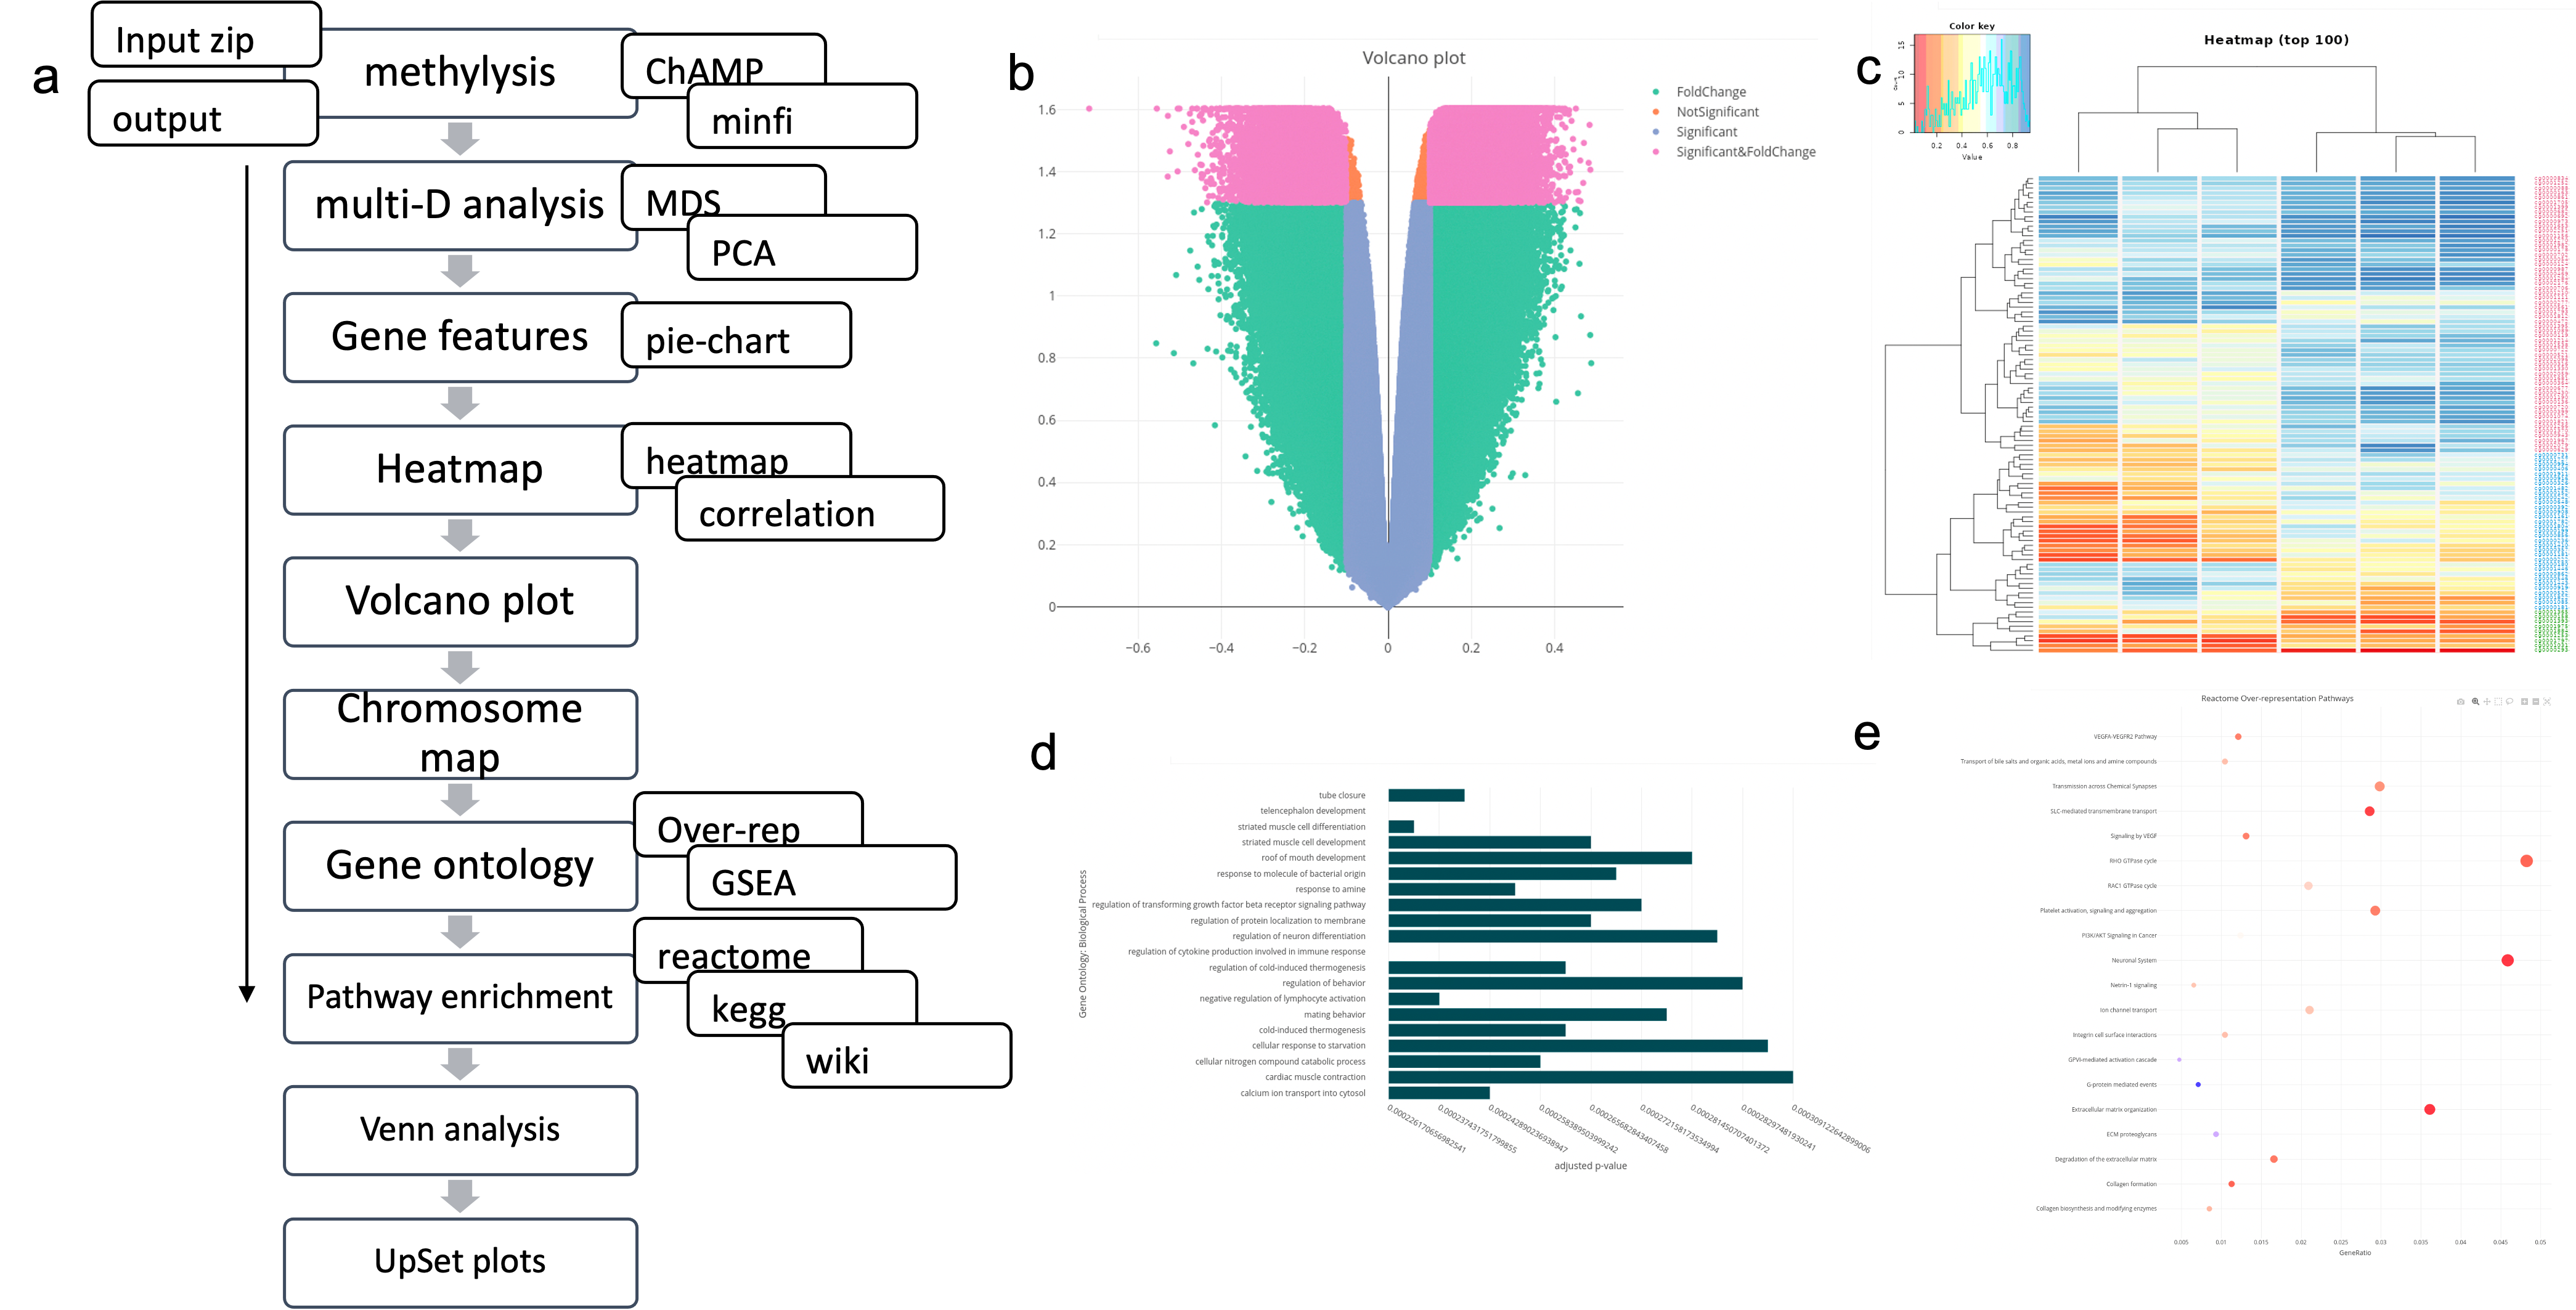
\includegraphics{images/Figure1.png}

}

\caption{Pipeline description and Figures}

\end{figure}%

\section*{Requirements}\label{requirements}
\addcontentsline{toc}{section}{Requirements}

\markright{Requirements}

\begin{itemize}
\tightlist
\item
  \textbf{LinuxOS} - (AMD64)

  \begin{itemize}
  \tightlist
  \item
    \emph{Ubuntu 20.04LTS}
  \item
    \emph{Docker} (version 20.10.18)
  \item
    \emph{web-browser}: \emph{Firefox} (version 105)
  \end{itemize}
\item
  \textbf{MacOS} - (AMD64)

  \begin{itemize}
  \tightlist
  \item
    \emph{Monterey (version 12.5.1)}
  \item
    \emph{Docker} (version 20.10.17)
  \item
    \emph{Docker Desktop} (version 4.12.0)
  \item
    \emph{web-browsers}:

    \begin{itemize}
    \tightlist
    \item
      \emph{Google Chrome} (version 106),
    \item
      \emph{Firefox} (version 106),
    \item
      \emph{Apple Safari} (version 15.6.1)
    \end{itemize}
  \end{itemize}
\item
  \textbf{WindowsOS} - (AMD64)

  \begin{itemize}
  \tightlist
  \item
    \emph{Windows 10} (version 21H2)
  \item
    \emph{Docker} (version 20.10.20)
  \item
    \emph{Docker Desktop} (version 4.13.0)
  \item
    \emph{WSL2} - (\textbf{Ubuntu 20.04LTS})
  \item
    web-browsers:

    \begin{itemize}
    \tightlist
    \item
      Firefox (version 106),
    \item
      Google Chrome (version 107),
    \item
      Microsoft Edge (version 106).
    \end{itemize}
  \end{itemize}
\end{itemize}

\begin{tcolorbox}[enhanced jigsaw, coltitle=black, colback=white, title=\textcolor{quarto-callout-note-color}{\faInfo}\hspace{0.5em}{Note}, leftrule=.75mm, titlerule=0mm, colframe=quarto-callout-note-color-frame, toprule=.15mm, opacityback=0, arc=.35mm, breakable, rightrule=.15mm, colbacktitle=quarto-callout-note-color!10!white, bottomtitle=1mm, opacitybacktitle=0.6, left=2mm, bottomrule=.15mm, toptitle=1mm]

TranscriptR cannot run on
\href{https://en.wikipedia.org/wiki/List_of_ARM_processors}{ARM64
chipset} architecture.

\end{tcolorbox}

\section*{How to Use}\label{how-to-use}
\addcontentsline{toc}{section}{How to Use}

\markright{How to Use}

\subsection*{Local use}\label{local-use}
\addcontentsline{toc}{subsection}{Local use}

\emph{TranscriptR} is packed into docker container that is available
online. Please check the
\href{https://github.com/JD2112/transcriptr}{github link} to run the
container from your local computer.\\

\begin{tcolorbox}[enhanced jigsaw, coltitle=black, colback=white, title=\textcolor{quarto-callout-important-color}{\faExclamation}\hspace{0.5em}{Important}, leftrule=.75mm, titlerule=0mm, colframe=quarto-callout-important-color-frame, toprule=.15mm, opacityback=0, arc=.35mm, breakable, rightrule=.15mm, colbacktitle=quarto-callout-important-color!10!white, bottomtitle=1mm, opacitybacktitle=0.6, left=2mm, bottomrule=.15mm, toptitle=1mm]

Please remember, after start analyzing one transcriptome analysis run,
the `submit' button will be dectivated until refreshing the session. In
this case, the user needs to upload the data again for another analysis.

\end{tcolorbox}

\begin{tcolorbox}[enhanced jigsaw, coltitle=black, colback=white, title=\textcolor{quarto-callout-note-color}{\faInfo}\hspace{0.5em}{Note}, leftrule=.75mm, titlerule=0mm, colframe=quarto-callout-note-color-frame, toprule=.15mm, opacityback=0, arc=.35mm, breakable, rightrule=.15mm, colbacktitle=quarto-callout-note-color!10!white, bottomtitle=1mm, opacitybacktitle=0.6, left=2mm, bottomrule=.15mm, toptitle=1mm]

Note: If you want to run with the test data, Please download the
testdata from \href{www.google.com}{Coming soon\ldots{}}

\end{tcolorbox}

\chapter{Quality Analysis}\label{sec-seqqual}

\begin{tcolorbox}[enhanced jigsaw, coltitle=black, colback=white, title=\textcolor{quarto-callout-important-color}{\faExclamation}\hspace{0.5em}{IMPORTANT}, leftrule=.75mm, titlerule=0mm, colframe=quarto-callout-important-color-frame, toprule=.15mm, opacityback=0, arc=.35mm, breakable, rightrule=.15mm, colbacktitle=quarto-callout-important-color!10!white, bottomtitle=1mm, opacitybacktitle=0.6, left=2mm, bottomrule=.15mm, toptitle=1mm]

\textbf{PLEASE NOTE} WE INCLUDED THE POSSIBILITY OF THE HUMAN
TRANSCRIPTOME DATA ANALYSIS FROM THE SEQUENCE DATA. NONE OF THE OWNER OF
THE CODE OR DATA CENTER IS RESPONSIBLE FOR HANDLING THE HUMAN DATA. IT
IS UPTO THE USER IF THEY WANT TO USE THE ONLINE VERSION FOR HUMAN DATA
ANALYSIS.

\end{tcolorbox}

The \emph{Quality Analysis} is the first section in \emph{transcriptR}.
It allows the user to asses for the quality of the RNA-seq experiment.
For convenience, you can run the quality analysis without needing to run
the whole RNA-seq pipeline (look at the ``Transcriptome Analysis
section''). The quality assessment will run
\href{https://www.bioinformatics.babraham.ac.uk/projects/fastqc/}{FastQC}
and \href{https://multiqc.info/}{MultiQC} in background and the user
will get a complete MultiQC analysis report in \emph{html} format. You
can skip the quality analysis and run the main pipeline directly,
transcriptR will perform the quality assessment at the beginning of the
analysis.

\begin{figure}[H]

\centering{

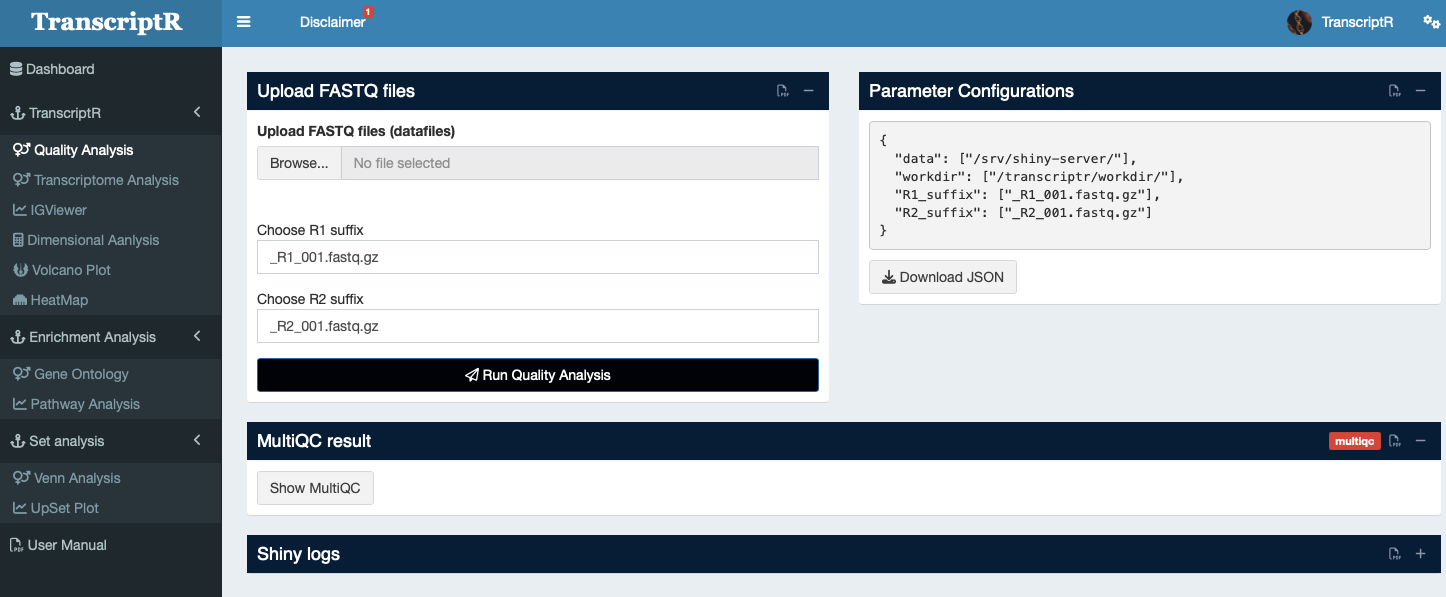
\includegraphics{images/quality/quality1.png}

}

\caption{\label{fig-qual1}Qaulity Analysis}

\end{figure}%

\section{How to use}\label{how-to-use-1}

Details are provided below -

\subsection{Data upload}\label{data-upload}

The current version can handle the upload of single fastq files. You can
select all of the fastq. User can browse through the folder to upload
data or drag \& drop files directly.

\begin{tcolorbox}[enhanced jigsaw, coltitle=black, colback=white, title=\textcolor{quarto-callout-note-color}{\faInfo}\hspace{0.5em}{Note}, leftrule=.75mm, titlerule=0mm, colframe=quarto-callout-note-color-frame, toprule=.15mm, opacityback=0, arc=.35mm, breakable, rightrule=.15mm, colbacktitle=quarto-callout-note-color!10!white, bottomtitle=1mm, opacitybacktitle=0.6, left=2mm, bottomrule=.15mm, toptitle=1mm]

Please note it will take some time to upload the data and once the data
uploaded, the list will be displayed in the browser (see
Figure~\ref{fig-qual2})

\end{tcolorbox}

\begin{figure}[H]

\centering{

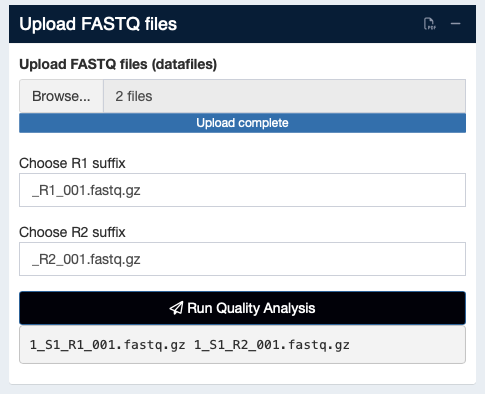
\includegraphics{images/quality/quality2.png}

}

\caption{\label{fig-qual2}Upload fastq}

\end{figure}%

\section{Parameters configurations}\label{parameters-configurations}

We provided the \textbf{\emph{JSON}} file (see Figure~\ref{fig-qual3})
to the user if they want to use the transcriptr snakemake pipeline by
their own. Please download a copy of your JSON file.

\begin{figure}[H]

\centering{

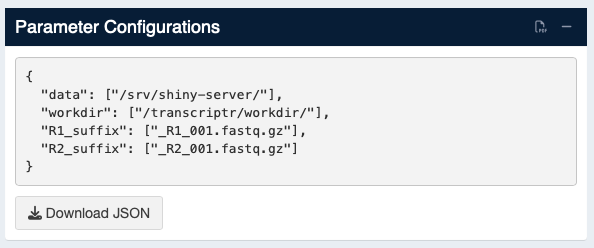
\includegraphics{images/quality/quality3.png}

}

\caption{\label{fig-qual3}JSON file for quality analysis}

\end{figure}%

\section{Run and Visualization}\label{run-and-visualization}

\subsection{Run Quality Analysis}\label{run-quality-analysis}

Once all fastq (\textbf{fastq.gz files only!}) files are uploaded on the
browser, please check the names and click \textbf{\emph{`Run Quality
Analysis'}} to submit the job.

\begin{tcolorbox}[enhanced jigsaw, coltitle=black, colback=white, title=\textcolor{quarto-callout-important-color}{\faExclamation}\hspace{0.5em}{Important}, leftrule=.75mm, titlerule=0mm, colframe=quarto-callout-important-color-frame, toprule=.15mm, opacityback=0, arc=.35mm, breakable, rightrule=.15mm, colbacktitle=quarto-callout-important-color!10!white, bottomtitle=1mm, opacitybacktitle=0.6, left=2mm, bottomrule=.15mm, toptitle=1mm]

Please remember, the \emph{fastqc} will use 12 cores in the background
to estimate the quality of the data. Make sure the computer has at least
16 cores.

\end{tcolorbox}

\subsection{Visualization}\label{visualization}

\subsubsection{Run logs}\label{run-logs}

We provided \textbf{\emph{`shiny logs'}} box Figure~\ref{fig-qual4} to
show the user the background run. It might be possible after submitting
the job, the browser hangs and cannot be reloaded. Please wait till the
background job finished. The \emph{sucess/failure} in the run will
appear in the \textbf{\emph{`shiny logs'}} box.

\begin{figure}[H]

\centering{

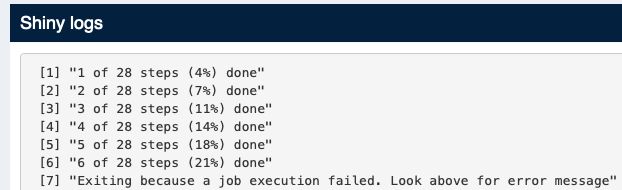
\includegraphics{images/quality/quality4.png}

}

\caption{\label{fig-qual4}shiny logs}

\end{figure}%

\subsubsection{Result - MultiQC}\label{result---multiqc}

Once the run sucessfully finished, the user can view the \emph{MultiQC}
result in the \textbf{\emph{MultiQC result}} box. Please click to
\emph{`show MultiQC'}.

\begin{figure}[H]

\centering{

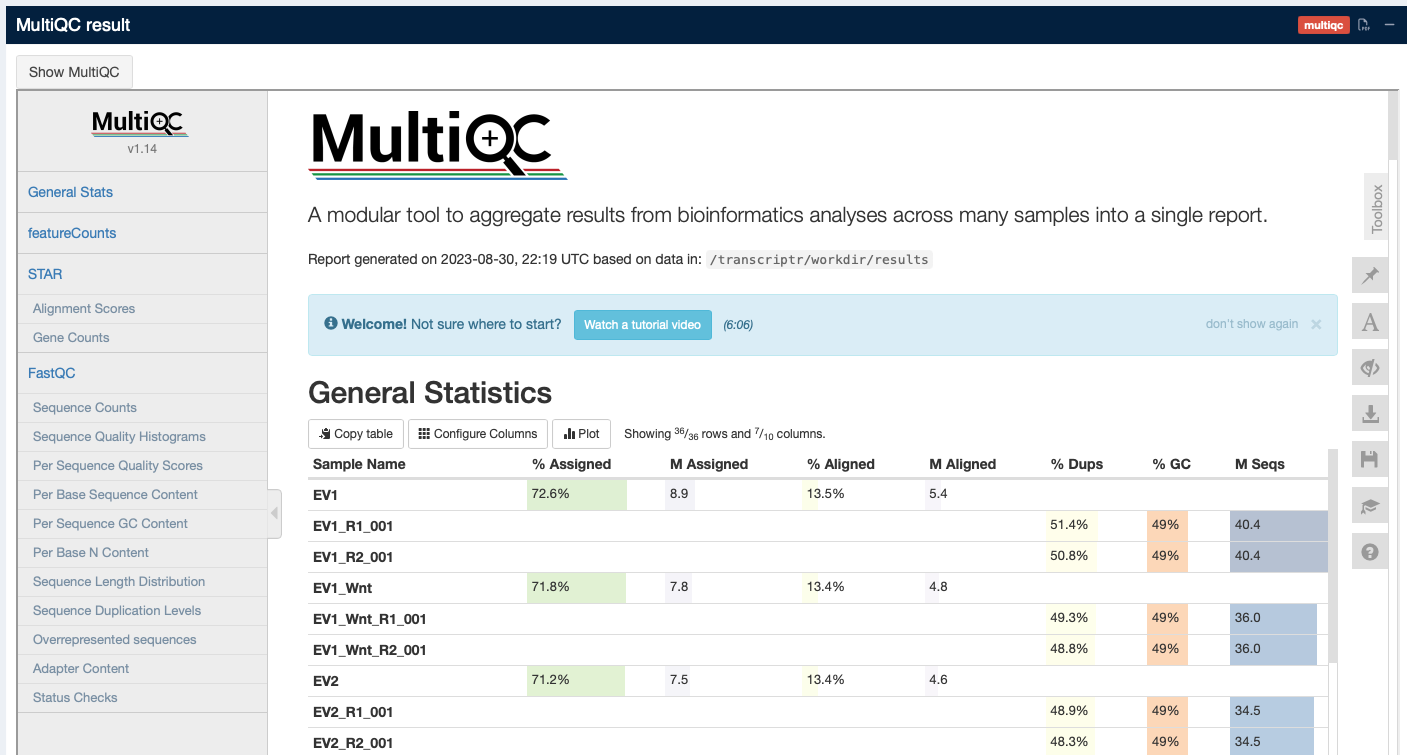
\includegraphics{images/quality/quality5.png}

}

\caption{\label{fig-qual5}MultiQC result}

\end{figure}%

\begin{tcolorbox}[enhanced jigsaw, coltitle=black, colback=white, title=\textcolor{quarto-callout-note-color}{\faInfo}\hspace{0.5em}{Note}, leftrule=.75mm, titlerule=0mm, colframe=quarto-callout-note-color-frame, toprule=.15mm, opacityback=0, arc=.35mm, breakable, rightrule=.15mm, colbacktitle=quarto-callout-note-color!10!white, bottomtitle=1mm, opacitybacktitle=0.6, left=2mm, bottomrule=.15mm, toptitle=1mm]

If \emph{MultiQC result} box cannot display any result (see
Figure~\ref{fig-qual5}), please reload the browser and check again. Make
sure all jobs finished successfully.

\end{tcolorbox}

\begin{tcolorbox}[enhanced jigsaw, coltitle=black, colback=white, title=\textcolor{quarto-callout-tip-color}{\faLightbulb}\hspace{0.5em}{Tip}, leftrule=.75mm, titlerule=0mm, colframe=quarto-callout-tip-color-frame, toprule=.15mm, opacityback=0, arc=.35mm, breakable, rightrule=.15mm, colbacktitle=quarto-callout-tip-color!10!white, bottomtitle=1mm, opacitybacktitle=0.6, left=2mm, bottomrule=.15mm, toptitle=1mm]

Check the
\href{https://github.com/JD2112/methylr/tree/main/data}{github}
repository for sample data file. You may download the Sample\_sheet.csv
file and use as a template for your sample\_sheet.

\end{tcolorbox}

\chapter{Transcriptome Analysis}\label{sec-transcript}

\begin{tcolorbox}[enhanced jigsaw, coltitle=black, colback=white, title=\textcolor{quarto-callout-important-color}{\faExclamation}\hspace{0.5em}{IMPORTANT}, leftrule=.75mm, titlerule=0mm, colframe=quarto-callout-important-color-frame, toprule=.15mm, opacityback=0, arc=.35mm, breakable, rightrule=.15mm, colbacktitle=quarto-callout-important-color!10!white, bottomtitle=1mm, opacitybacktitle=0.6, left=2mm, bottomrule=.15mm, toptitle=1mm]

\textbf{PLEASE NOTE} WE INCLUDED THE POSSIBILITY OF THE HUMAN
TRANSCRIPTOME DATA ANALYSIS FROM THE SEQUENCE DATA. NONE OF THE OWNER OF
THE CODE OR DATA CENTER IS RESPONSIBLE FOR HANDLING THE HUMAN DATA. IT
IS UPTO THE USER IF THEY WANT TO USE THE ONLINE VERSION FOR HUMAN DATA
ANALYSIS.

\end{tcolorbox}

Transcriptome analysis has divided in several parts for the data upload,
analysis and visualizing the results.

\section{Data input and parameters
settings}\label{data-input-and-parameters-settings}

In this section, for better user accessibility, we divided this into 3
sub-parts -

\begin{figure}[H]

\centering{

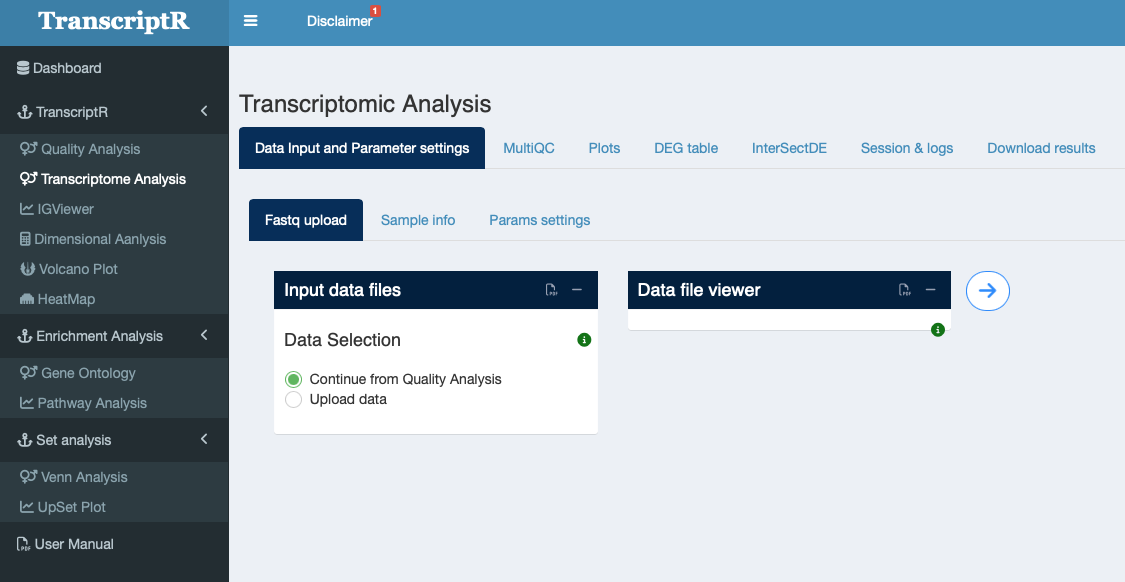
\includegraphics{images/transcriptome/transcript1.png}

}

\caption{\label{fig-trans1}Fastq upload}

\end{figure}%

\subsection{Fastq upload}\label{fastq-upload}

\begin{enumerate}
\def\labelenumi{\arabic{enumi}.}
\tightlist
\item
  If the user performed the \textbf{\emph{Quality analysis}}
  (Chapter~\ref{sec-seqqual}) already, they don't need to upload the
  data again, they can use \textbf{\emph{`continue from Quality
  Analysis'}}.
\item
  The user can also upload the data directly by selecting
  \textbf{\emph{`upload data'}} option.
\end{enumerate}

\begin{tcolorbox}[enhanced jigsaw, coltitle=black, colback=white, title=\textcolor{quarto-callout-note-color}{\faInfo}\hspace{0.5em}{Note}, leftrule=.75mm, titlerule=0mm, colframe=quarto-callout-note-color-frame, toprule=.15mm, opacityback=0, arc=.35mm, breakable, rightrule=.15mm, colbacktitle=quarto-callout-note-color!10!white, bottomtitle=1mm, opacitybacktitle=0.6, left=2mm, bottomrule=.15mm, toptitle=1mm]

Please note it will take some time to upload the data and once the data
uploaded, the list will be displayed in the \textbf{Data file viewer}
(see Figure~\ref{fig-qual2} Figure~\ref{fig-trans1}).

\end{tcolorbox}

\subsection{Sample info}\label{sec-sampleinfo}

In the \textbf{\emph{Sample info}} section, users need to upload the
`sample sheet/meta data file' that includes atleast two columns (`sample
name' and `sample condition') (see Figure~\ref{fig-trans2}). For
Differential Gene Expression (DEG) analysis, user need to provide the
comparison conditions as showed in Figure~\ref{fig-trans2}.

\begin{figure}[H]

\centering{

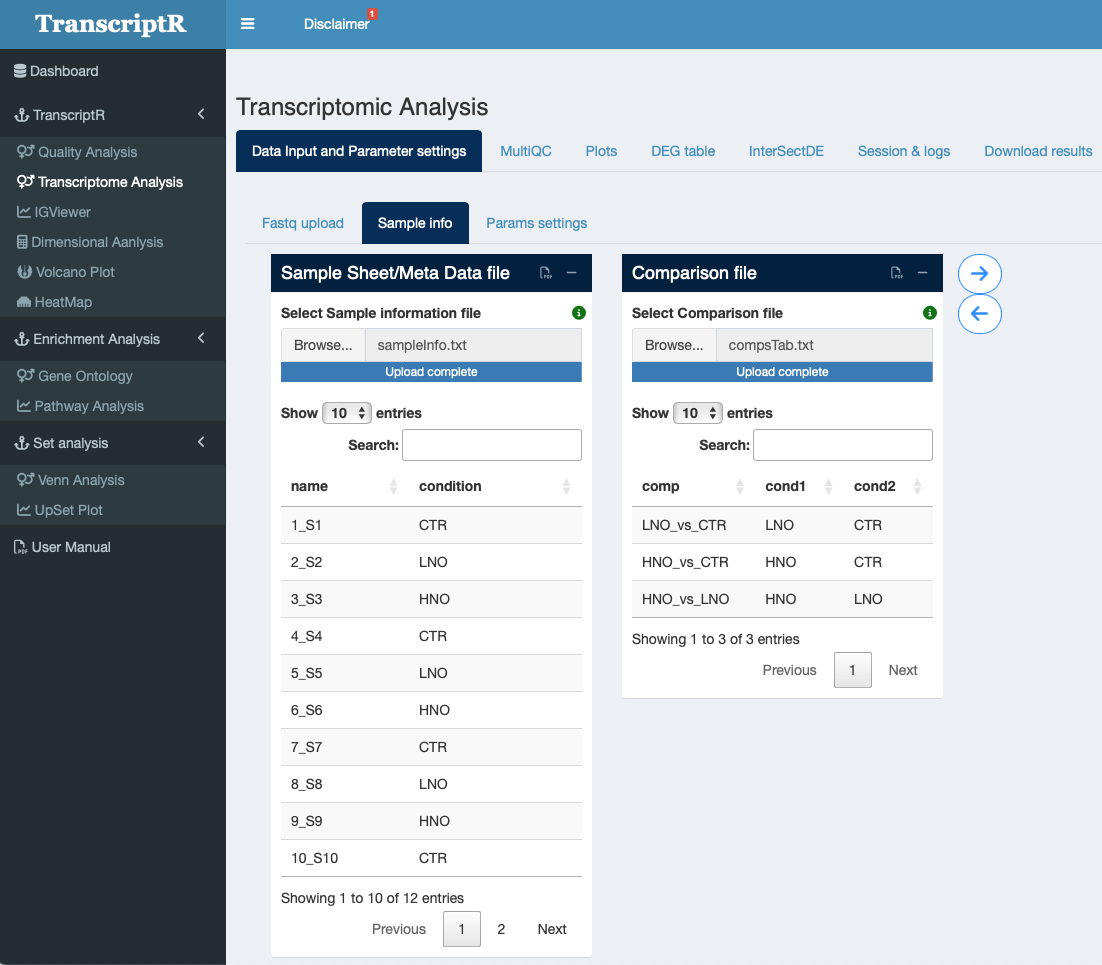
\includegraphics{images/transcriptome/transcriptr3.png}

}

\caption{\label{fig-trans2}Sample information}

\end{figure}%

\begin{tcolorbox}[enhanced jigsaw, coltitle=black, colback=white, title=\textcolor{quarto-callout-tip-color}{\faLightbulb}\hspace{0.5em}{Tip}, leftrule=.75mm, titlerule=0mm, colframe=quarto-callout-tip-color-frame, toprule=.15mm, opacityback=0, arc=.35mm, breakable, rightrule=.15mm, colbacktitle=quarto-callout-tip-color!10!white, bottomtitle=1mm, opacitybacktitle=0.6, left=2mm, bottomrule=.15mm, toptitle=1mm]

\begin{enumerate}
\def\labelenumi{\arabic{enumi}.}
\tightlist
\item
  After uploading the files, all files will be appear in the browser
  window (see Figure~\ref{fig-trans2}), please check and verify
  everything is properly uploaded.
\item
  User can upload any file format, such as text (.txt), CSV (.csv),
  Excel (.xls, .xlsx).
\end{enumerate}

\end{tcolorbox}

\subsection{Parameters settings}\label{parameters-settings}

Selecting the right parameters for the analysis is the key to the
successful run of \textbf{TranscriptR}. The \textbf{parameters settings}
(see Figure~\ref{fig-trans3}) are sub-divided for better understanding
and view -

\begin{figure}[H]

\centering{

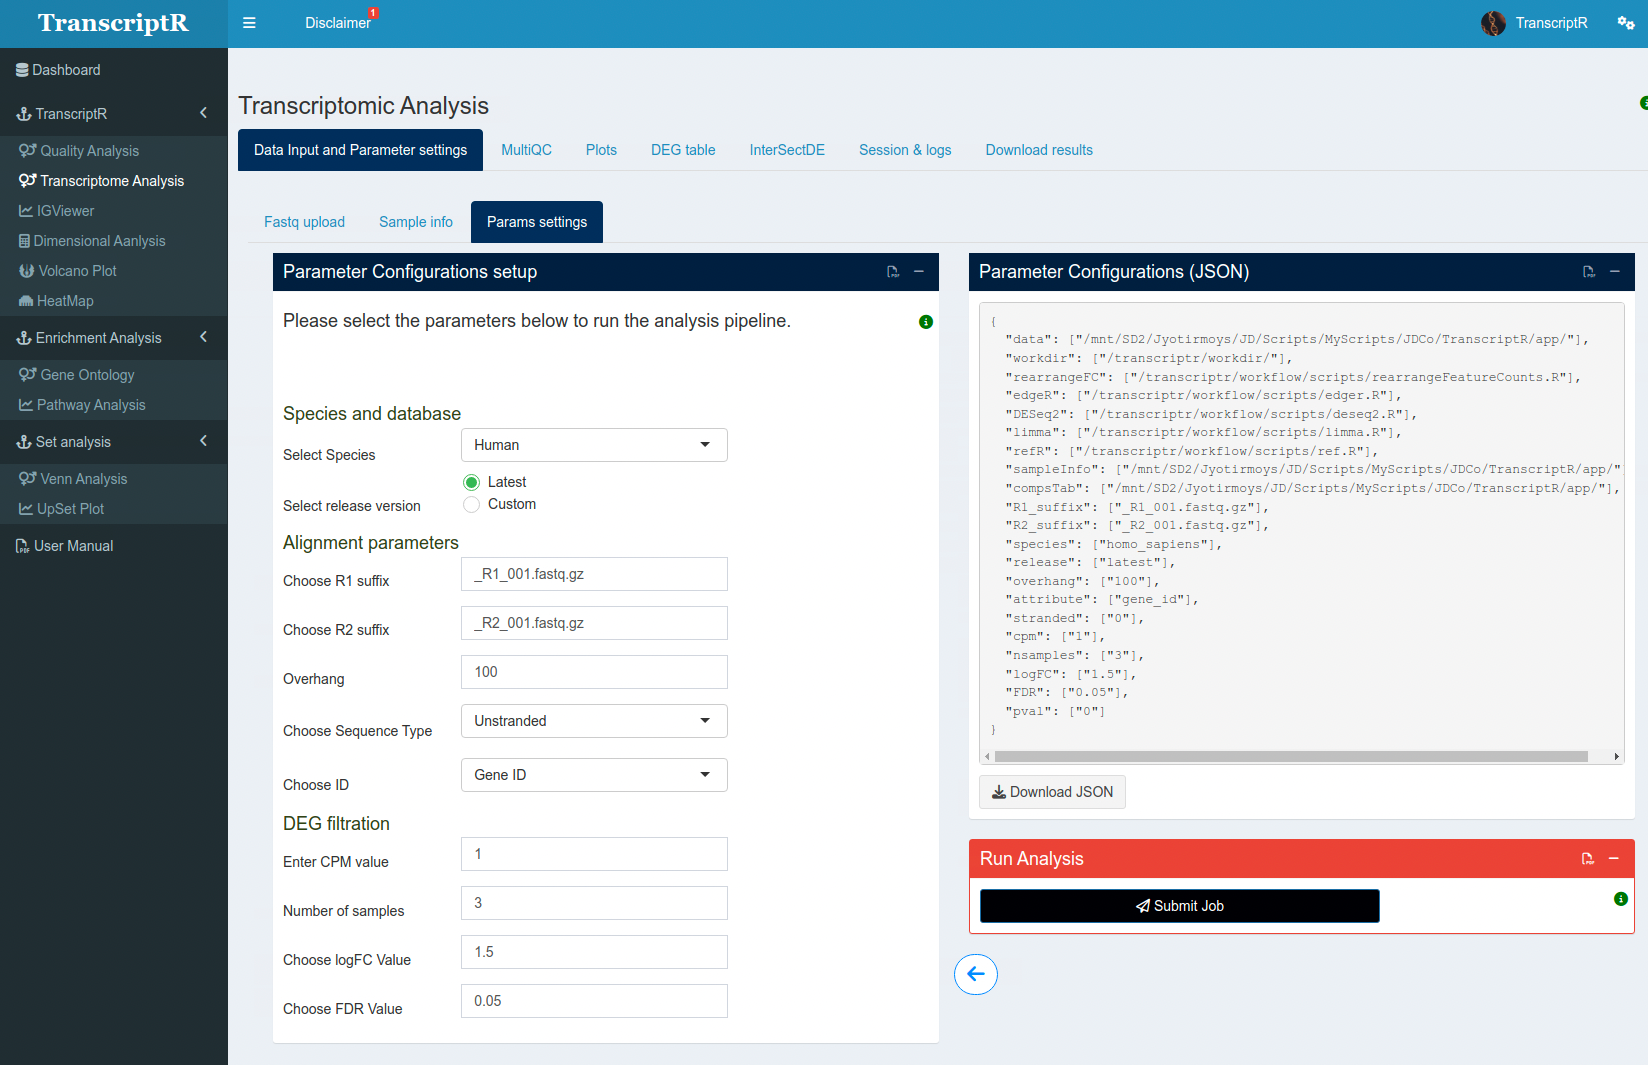
\includegraphics{images/transcriptome/transcriptr4.png}

}

\caption{\label{fig-trans3}Parameters settings}

\end{figure}%

\subsubsection{Species and database}\label{species-and-database}

\begin{enumerate}
\def\labelenumi{\arabic{enumi}.}
\tightlist
\item
  \textbf{Select Species}: The user need to select the \emph{species}
  from the species list. Here we provided more than 350 species
  presented in the `biomart' for the analysis. Note that all other
  species than `Human', `Mouse' and `Rat' come with the
  \textbf{scientific name} as provided in
  \href{http://www.ensembl.org/info/about/species.html}{`Ensembl'}. The
  default is `Human'.
\item
  \textbf{Select release version}: The default is \emph{latest}. The
  user can choose other database version as provided by
  \href{https://ftp.ensembl.org/pub/}{Ensembl}. Please provide the
  number only in the `box', example, if you want to use version `109',
  provide only `109' (see Figure~\ref{fig-trans4}).
\end{enumerate}

\begin{figure}[H]

\centering{

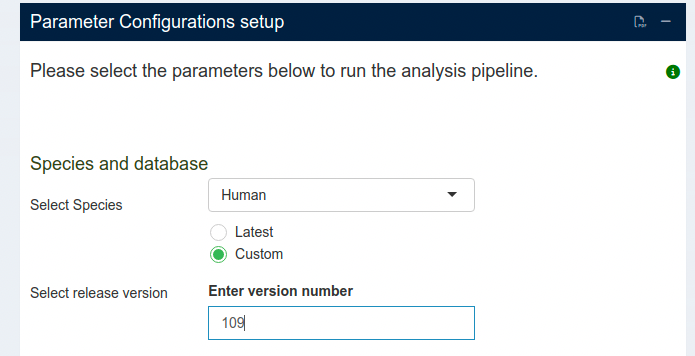
\includegraphics{images/transcriptome/transcript5.png}

}

\caption{\label{fig-trans4}Parameters: Species and database}

\end{figure}%

\subsubsection{Alignment parameters}\label{alignment-parameters}

\begin{enumerate}
\def\labelenumi{\arabic{enumi}.}
\tightlist
\item
  \textbf{Choose R1/R2 suffix}: For \emph{paired-end} analysis, please
  provide the R1 and R2 suffixes.
\item
  \textbf{Overhang}: The default is 100.
\item
  \textbf{Choose sequence type}: Choose whether the sequence is
  \emph{stranded}, \emph{unstranded} or \emph{reverse-stranded}.
\item
  \textbf{Choose ID}: Select display ID for \emph{gene id} or
  \emph{transcriptome id}. Default is \emph{gene ID}.
\end{enumerate}

\begin{figure}[H]

\centering{

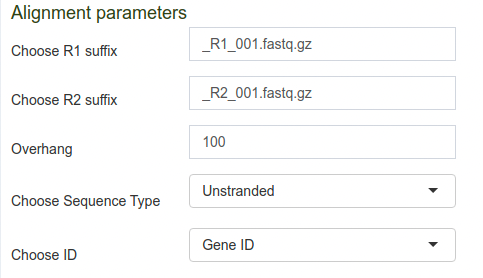
\includegraphics{images/transcriptome/transcript6.png}

}

\caption{\label{fig-trans5}Parameters: Alignment}

\end{figure}%

\subsubsection{DEG filtration}\label{deg-filtration}

As \textbf{`TranscriptR'} provides the differential gene expression
(DEG) analysis result, user need to provide the required filtration for
the analysis.\\
1. \textbf{Enter CPM value}: The default is 1.\\
2. \textbf{Number of samples}: The default is 3.\\
3. \textbf{Choose logFC value}: The default is 1.5.\\
4. \textbf{Choose FDR value}: The default is 0.05.

\begin{figure}[H]

\centering{

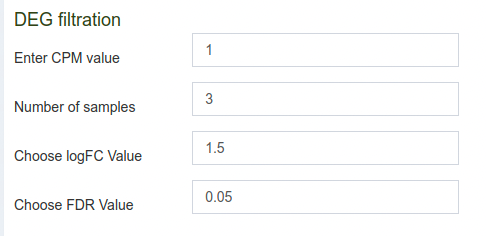
\includegraphics{images/transcriptome/transcript7.png}

}

\caption{\label{fig-trans6}Parameters: DEF filtration}

\end{figure}%

\section{Visualization: MultiQC}\label{visualization-multiqc}

Please see Chapter~\ref{sec-seqqual} for details.

\section{Visualization: Plots}\label{visualization-plots}

Since \textbf{TranscriptR} provides differential gene expression (DEG)
analysis by \textbf{three} different pipelines, namely \emph{EdgeR},
\emph{DESeq2} and \emph{limma}, all plots are divided into these three
results.

\begin{figure}[H]

\centering{

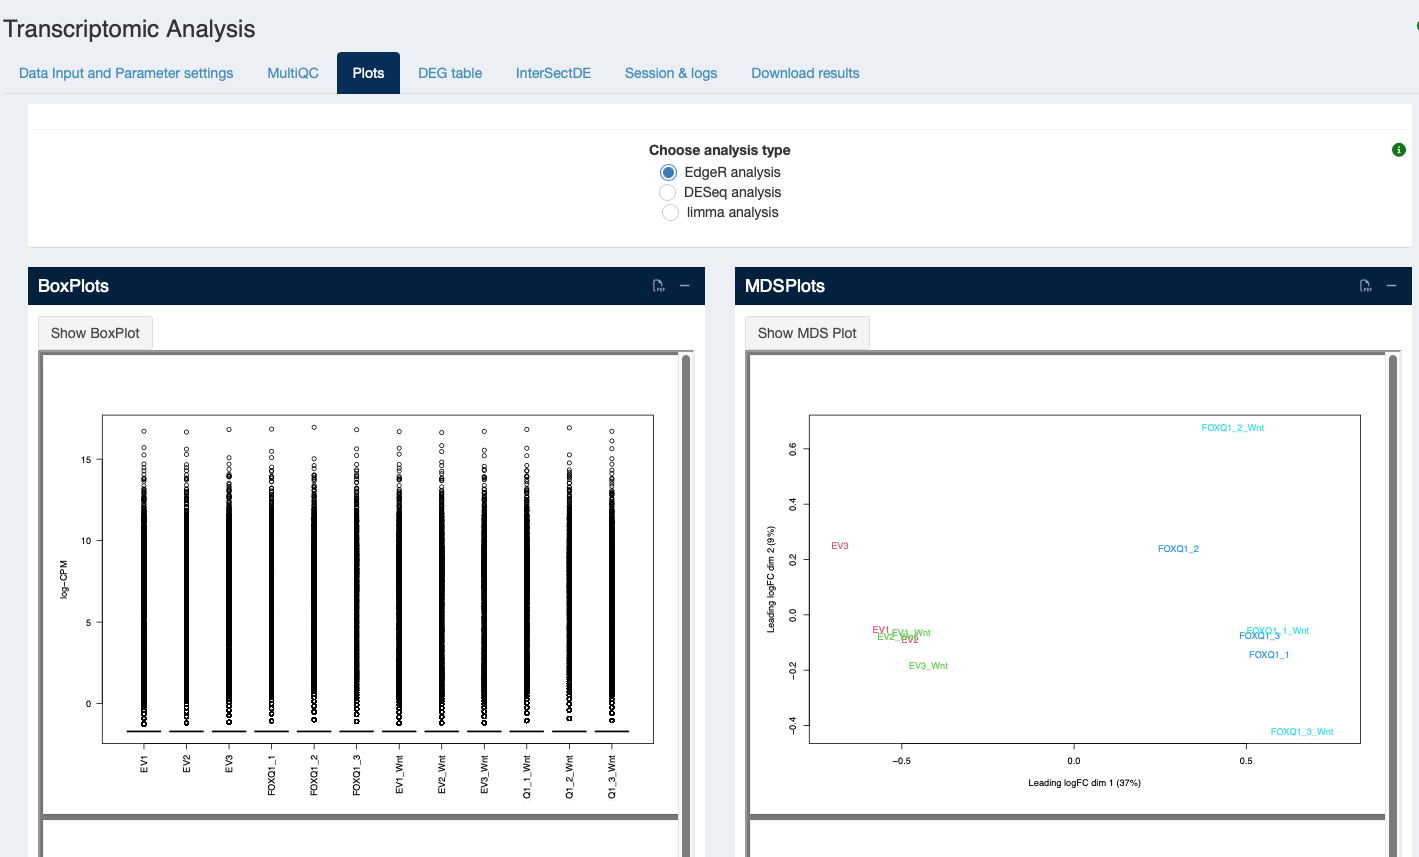
\includegraphics{images/transcriptome/transcript8.png}

}

\caption{\label{fig-trans7}Visualization: plots}

\end{figure}%

\begin{tcolorbox}[enhanced jigsaw, coltitle=black, colback=white, title=\textcolor{quarto-callout-note-color}{\faInfo}\hspace{0.5em}{Note}, leftrule=.75mm, titlerule=0mm, colframe=quarto-callout-note-color-frame, toprule=.15mm, opacityback=0, arc=.35mm, breakable, rightrule=.15mm, colbacktitle=quarto-callout-note-color!10!white, bottomtitle=1mm, opacitybacktitle=0.6, left=2mm, bottomrule=.15mm, toptitle=1mm]

\begin{enumerate}
\def\labelenumi{\arabic{enumi}.}
\tightlist
\item
  The plots will be displayed as Figure~\ref{fig-trans7} in a PDF
  format. All of these can be downloaded when the user download the
  results from the \emph{`Download results'} tab.
\item
  Please note, if the plots are not loaded after the \emph{job}
  completed and clicked on `show BoxPlot/Show MDS Plot' button, refresh
  the browser and it will appear in the box.
\end{enumerate}

\end{tcolorbox}

\section{Visualization: DEG table}\label{visualization-deg-table}

We provided differential gene expression (DEG) analysis result as a
table format (see Figure~\ref{fig-trans8}). To display the table, user
need to - ~ 1. choose the analysis type (as \textbf{TranscriptR}
provides three different pipeline results), such as \emph{EdgeR
analysis}, \emph{DESeq analysis} or \emph{limma analysis} and\\
2. select DEG table from the drop-down list. The list is generated from
the information provided by the \emph{comparison table}.

\begin{figure}[H]

\centering{

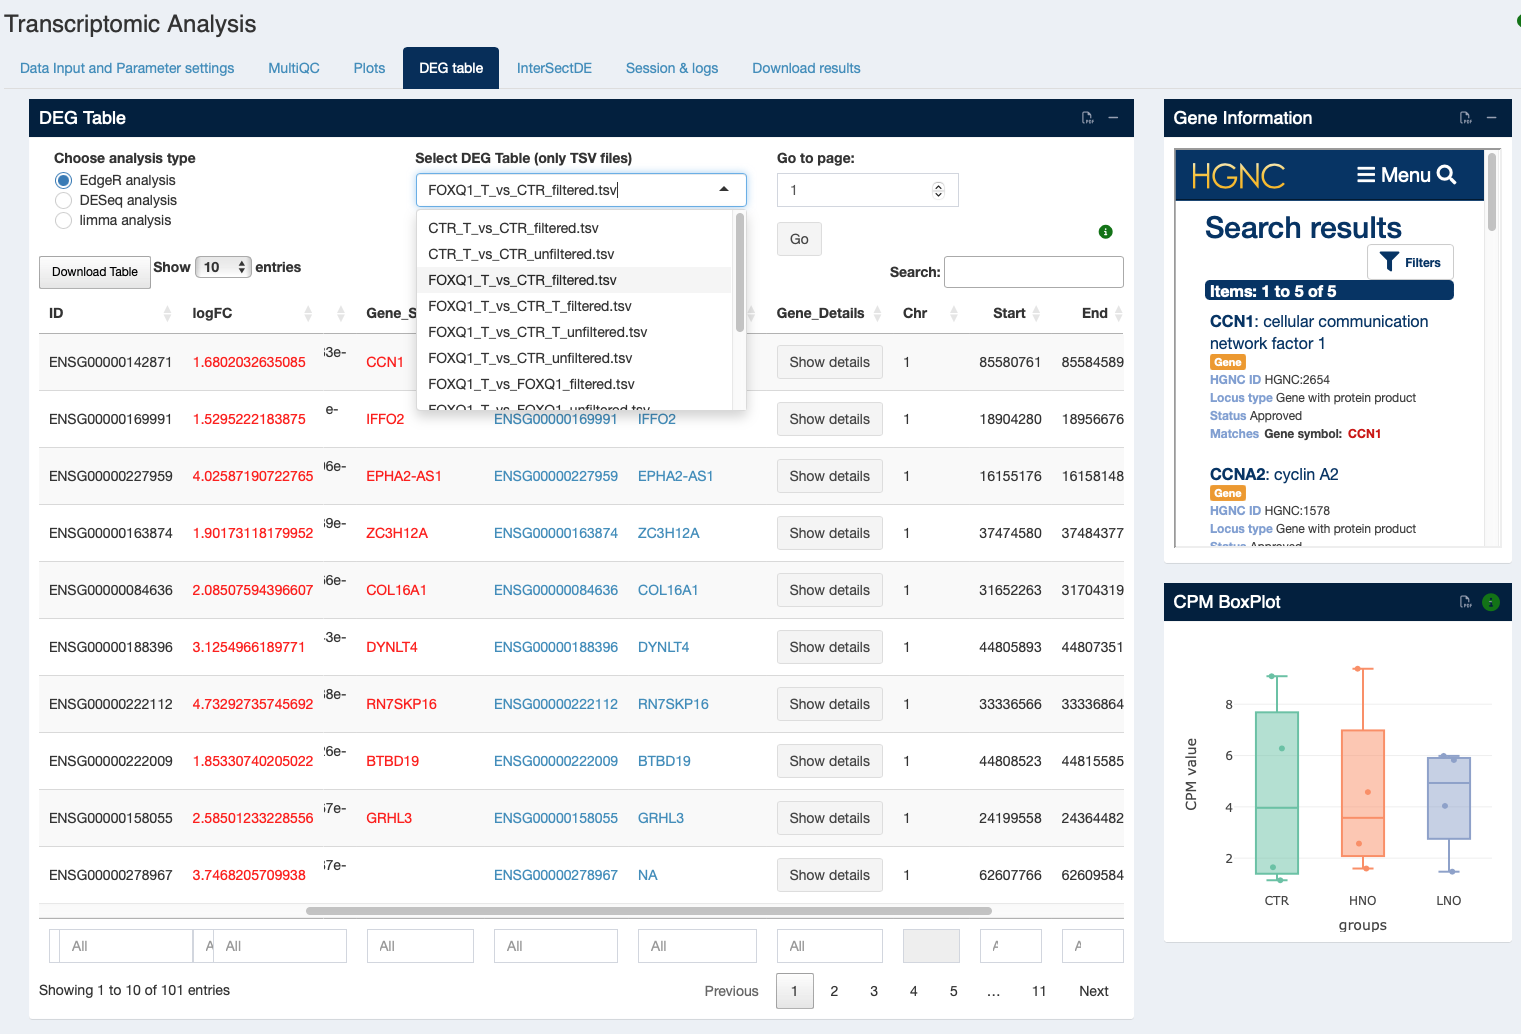
\includegraphics{images/transcriptome/transcript9.png}

}

\caption{\label{fig-trans8}Visualization: DEG table}

\end{figure}%

In the DEG table, we added information for -\\
1. \textbf{ID}: ENSEMBL \emph{gene ID} or \emph{transcript ID}\\
2. \textbf{logFC}: log fold change value for each ID. Red color shows
the higher expression and blue represents the low expression (same
corresponds to \emph{gene symbol}).\\
3. \textbf{logCPM}: log CPM value provided\\
4. \textbf{P\_value}: \emph{p}-value provided for each ID.\\
5. \textbf{FDR}: FDR provided for each ID.\\
6. \textbf{Gene Symbol}: official gene symbol added in the table.
Coloured according to the \emph{logFC} value.\\
7. \textbf{Ensembl link}: we added external link for ensembl database to
view further information on the ID.\\
8. \textbf{GeneCard link}: we added genecard database link for more
information on the ID.\\
9. \textbf{Gene details}: Clicking on \emph{'show details} button will
result to display the boxplot of CPM data for each group (\textbf{see
the note below}) and the gene information from \textbf{HGNC} (human
only).\\
10. \textbf{Chr}: Chromosomal location\\
11. \textbf{Start}: Start position of the chromosome\\
12. \textbf{End}: End position of the chromosome\\
13. \textbf{Strand}: chromosomal strand\\
14. \textbf{Types}: types of genes/transcript.

\begin{tcolorbox}[enhanced jigsaw, coltitle=black, colback=white, title=\textcolor{quarto-callout-important-color}{\faExclamation}\hspace{0.5em}{Important}, leftrule=.75mm, titlerule=0mm, colframe=quarto-callout-important-color-frame, toprule=.15mm, opacityback=0, arc=.35mm, breakable, rightrule=.15mm, colbacktitle=quarto-callout-important-color!10!white, bottomtitle=1mm, opacitybacktitle=0.6, left=2mm, bottomrule=.15mm, toptitle=1mm]

Please note, we already mentioned that the user may need to
reload/refresh the browser after successful run to visualize the
results. In this process, the uploaded data table (\textbf{mentioned in
Section~\ref{sec-sampleinfo}}) will be lost. To view the CPM boxplot,
the user need the upload the sample information data tables again and
click on \emph{`Show details'} on the DEG table.

\end{tcolorbox}

\section{Visualization: InterSectDE}\label{visualization-intersectde}

Further, we implemented intersection function for the above-mentioned
three types of DEG analyses in the \emph{'InterSectDEG} tab.\\
1. To visualize the result, the user needs to select the \emph{same
result} table (eg. groupAvsgroupB) for all three analyses.
\textbf{Please remember selecting different table may results incorrect
table and figure.\\
2. After selecting same result table files from all three analyses,
click to \emph{`show intersect result'}. Both intersect table and Venn
diagram will appear in respective boxes.\\
3. To download the full table, check to show }all** entries (see
Figure~\ref{fig-trans9}).\\
4. The Venn diagram can be downloaded in different file format with
respective height, width or resolution (see Figure~\ref{fig-trans9}).

\begin{figure}[H]

\centering{

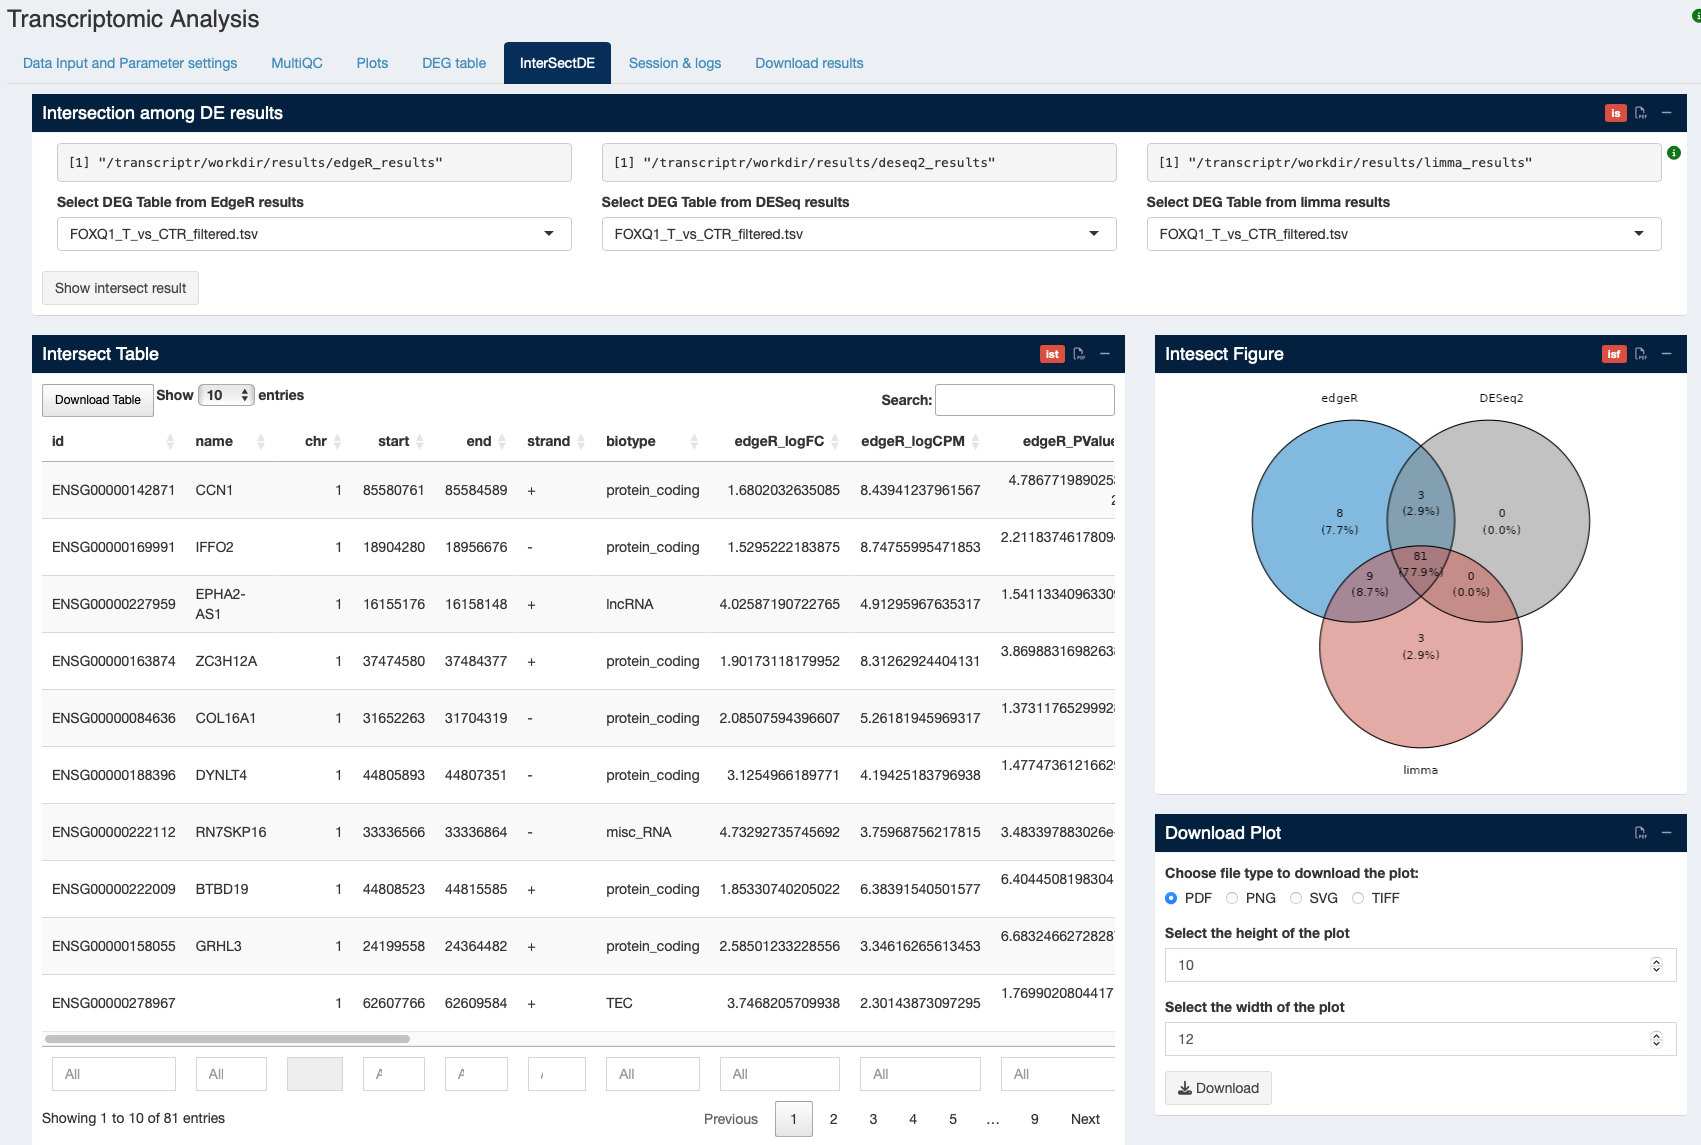
\includegraphics{images/transcriptome/transcript10.png}

}

\caption{\label{fig-trans9}InterSect result}

\end{figure}%

Below is the details of \emph{`InterSect DEG'} table result (see
Figure~\ref{fig-trans9}) -\\
1. \textbf{id}\\
2. \textbf{name}\\
3. \textbf{chr}\\
4. \textbf{start}\\
5. \textbf{end}\\
6. \textbf{strand}\\
7. \textbf{biotype}\\
8. \textbf{edgeR\_logFC}\\
9. \textbf{edgeR\_logCPM}\\
10. \textbf{edgeR\_PValue}\\
11. \textbf{edgeR\_FDR}\\
12. \textbf{edgeR\_baseMean}\\
13. \textbf{DESeq2\_log2FoldChange}\\
14. \textbf{DESeq2\_lfcSE}\\
15. \textbf{DESeq2\_stat}\\
16. \textbf{DESeq2\_pvalue}\\
17. \textbf{DESeq2\_padj}\\
18. \textbf{limma\_logFC}\\
19. \textbf{limma\_AveExpr}\\
20. \textbf{limma\_t}\\
21. \textbf{limma\_P.Value}\\
22. \textbf{limma\_adj.P.Val}\\
23. \textbf{limma\_B}

\section{Session \& logs}\label{session-logs}

We included the next tab to show \emph{`GTF information'},
\emph{`Reference information'}, \emph{`Shiny logs'} and \emph{`Session
information'} for the pipeline run.

\section{Download Results}\label{download-results}

In the \emph{`Download results'} tab, user can download all results
performed and saved during the \textbf{Transcriptome Analysis} run in a
zip folder. This also contains the snakemake and session logs.

\chapter{Integrative Genome Viewer}\label{integrative-genome-viewer}

Thanks to \textbf{IGV-Shiny}, we have included a sub-section to
visualize the BedGraph result in the genome viewer.

\section{Parameters and Genome View}\label{parameters-and-genome-view}

\begin{enumerate}
\def\labelenumi{\arabic{enumi}.}
\tightlist
\item
  Please select the \emph{`bedgraph'} file from the drop-down list.
\item
  \emph{`Run IGV'} and it will create the chromosome map on the side
  box, \emph{`genome view'}.
\item
  In the \emph{`Genome View'} box, select the chromosome number in
  interest.
\item
  Click on \emph{`Add as BedGraph'} to view the result on the chromosome
  level.
\item
  Use cursor to zoom in/out on the location/region.
\end{enumerate}

\begin{figure}[H]

\centering{

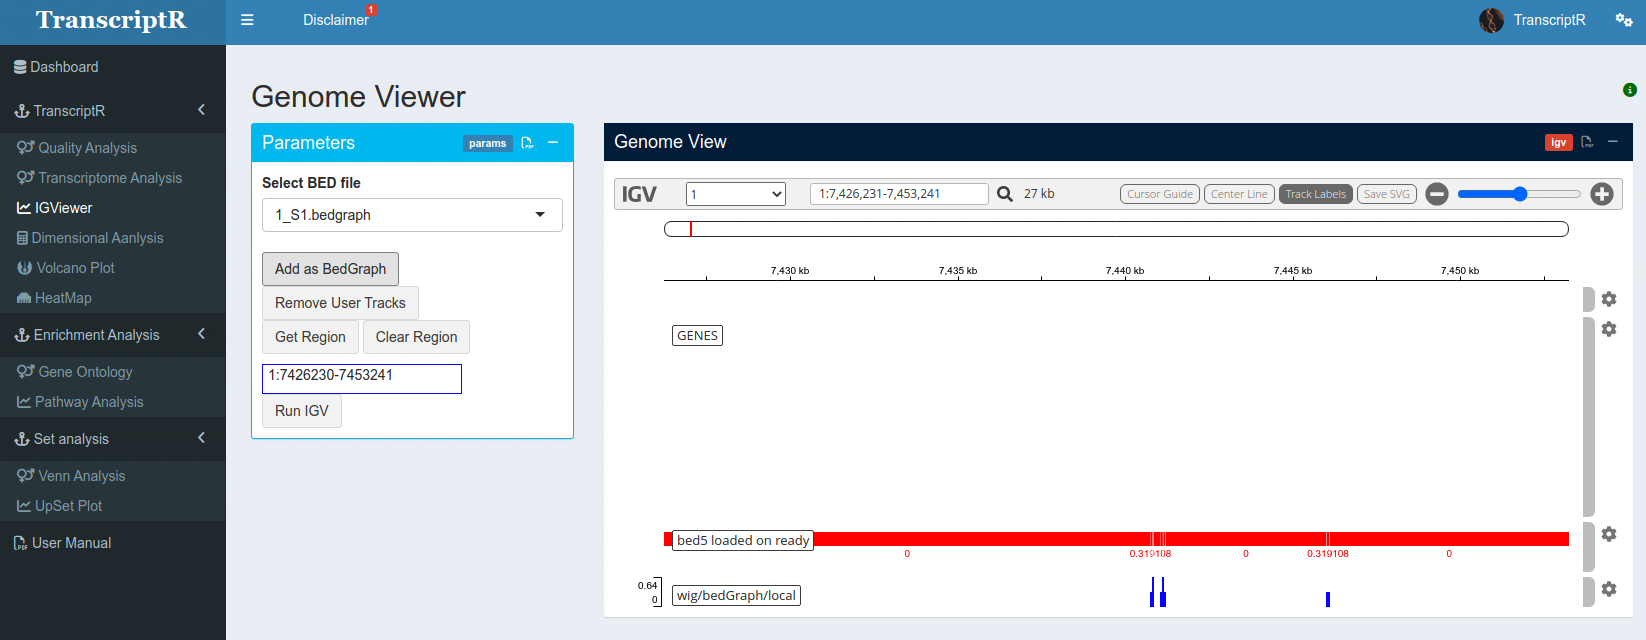
\includegraphics{images/igv/igv1.png}

}

\caption{\label{fig-igv1}Genome View}

\end{figure}%

\chapter{Dimensional Analysis}\label{sec-multid}

\footnote{TO ALL OUR USERS, IF YOU ARE EXPERIENCING ANY TROUBLE WITH THE
  APP, BEFORE SENDING THE BUG REPORT, PLEASE RESTART THE DOCKER
  CONTAINER AND TRY AGAIN.}

In \emph{TranscriptR}, multiple dimensional analysis includes two type
of analysis -\\
1. \textbf{MDS}: Multidimensional Scaling\\
2. \textbf{PCA}: Prinicipal Component Analysis

Multidimensional scaling is a visual representation of distances or
dissimilarities between set of objects. \textbf{MDS} finds set of
vectors in \emph{p}-dimensional space such that the matrix of Euclidean
distance among them corresponds as closely as possible to some function
of the input matrix. The input to multidimensional scaling is a distance
matrix. To get some more details on how to use \textbf{MDS} in
biological data, read
\autocite{mugavin2008multidimensional,lacher1987interpretation,lacher1988comparison}\\
Principal Component Analysis (PCA) is the original vectors in
n-dimensional space and the data are projected onto the directions in
the data with the most variance.

\section{MDS}\label{mds}

\subsection{How to use}\label{how-to-use-2}

For both analysis, user need to provide a \textbf{TEXT (tab-delimited)
file with numeric values}, \emph{e.g.} the output normalized (CPM) table
from `Transcriptome Analysis'. However the user can use similar tables
for the analysis.

\subsubsection{Data Upload}\label{data-upload-1}

\begin{enumerate}
\def\labelenumi{\arabic{enumi}.}
\tightlist
\item
  User can choose the option to use number of variables from the
  uploaded data file.
\item
  User can change the size of the points by using \emph{`select size'}.
\item
  User can choose where to show which dimension (e.g.~Select X/Y (axis)
  dimension - 1,2,3, etc.). Default is Dimension 1 for X-axis and
  Dimension 2 for Y-axis.
\item
  Next, the user can change the label of X and Y-axis.
\item
  Select the text file (tab-delimited file) and upload it.
\item
  In addition, we added the option to colour the groups. The user needs
  to upload the group file - one column file with different group names
  (same as number of samples).
\item
  To group the colour, the user needs to specify the number of groups.
  At present, maximum 10 groups can be coloured.
\end{enumerate}

\subsubsection{Analysis result}\label{analysis-result}

\begin{enumerate}
\def\labelenumi{\arabic{enumi}.}
\tightlist
\item
  After the click on ``Run MDS Analysis'', the program will take some
  time to generate the plot and will appear as soon the run finishes.
  The zoom bar can be used to zoom in/out the plot.
\item
  The generated figure can be downloaded in different format, vector
  graphics support - PDF and SVG or PNG and TIFF. User can download all
  different options for the same figure.\\
\end{enumerate}

\section{PCA plot}\label{pca-plot}

\subsection{Data Upload}\label{data-upload-2}

\begin{enumerate}
\def\labelenumi{\arabic{enumi}.}
\tightlist
\item
  User can choose the option to use \emph{number of most variables}
  (default is 1000) from the uploaded data file.
\item
  User can change the size of the points by using \emph{`select size'}
  (default is 1).
\item
  User can write their own \emph{Main title} for the plot (e.g., PCA
  plot).
\item
  User can write the \emph{legend title} for the plot (e.g., Groups).
\item
  Next, the user can change the label of X and Y-axis.
\item
  User can choose to show the \emph{`Mean point'}. The mean point
  calculates the mean value of the respective group and plot them.
\item
  User can \emph{`Select Colour Palette'} from the drop-down list.
\item
  Select the text file (tab-delimited file) and upload it.
\item
  User needs to \emph{`Upload group file'} (same as MDS) and \emph{`Run
  PCA Analysis'}.
\end{enumerate}

\subsection{Analysis Result}\label{analysis-result-1}

\begin{enumerate}
\def\labelenumi{\arabic{enumi}.}
\tightlist
\item
  The generated plot is dynamic and positional details with the group
  name can be seen with mouse hovering.
\item
  The plot is generated using the plotly application, it can zoom
  in/out, save figure as PNG format, and do all other available
  functionality for plotly figures.
\item
  User can also download the dynamic figure as html file.
\end{enumerate}

\begin{tcolorbox}[enhanced jigsaw, coltitle=black, colback=white, title=\textcolor{quarto-callout-note-color}{\faInfo}\hspace{0.5em}{Note}, leftrule=.75mm, titlerule=0mm, colframe=quarto-callout-note-color-frame, toprule=.15mm, opacityback=0, arc=.35mm, breakable, rightrule=.15mm, colbacktitle=quarto-callout-note-color!10!white, bottomtitle=1mm, opacitybacktitle=0.6, left=2mm, bottomrule=.15mm, toptitle=1mm]

Please note that, the single column with header \textbf{``group''}
should be supplied in this file. Match the column names of the variable
data file with the group.\\
\textbf{\emph{Example:}} If in the variable data file, the column names
are - sampleA1 sampleA2 sampleA3 sampleB1 sampleB2 sampleB3 the group
text file should be like this - group\\
A\\
A\\
A\\
B\\
B\\
B\\
For more, please see the
\href{https://sourceforge.net/projects/TranscriptR/}{test data} files.

\end{tcolorbox}

\begin{figure}[H]

{\centering 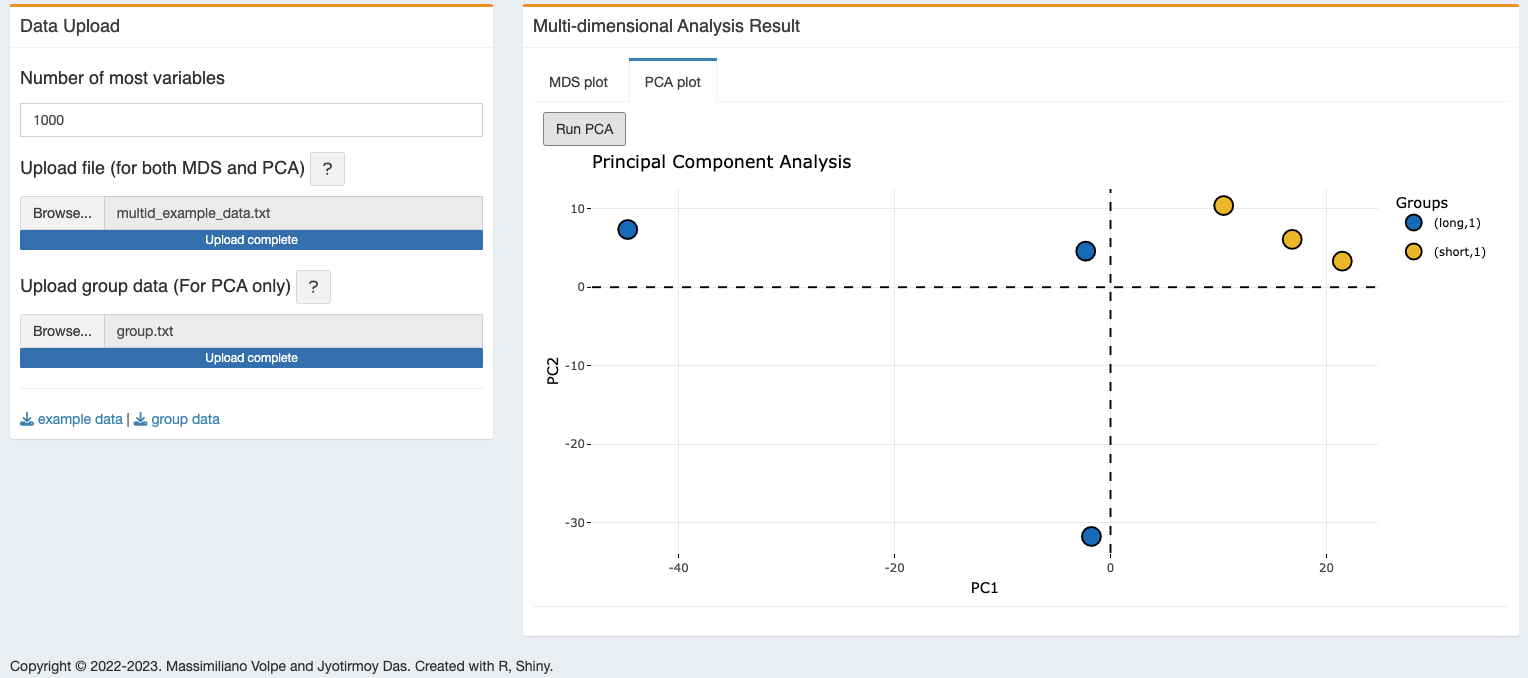
\includegraphics{images/PCA.png}

}

\caption{Principal Component Analysis plot}

\end{figure}%

\section{R packages used}\label{r-packages-used}

\begin{enumerate}
\def\labelenumi{\arabic{enumi}.}
\tightlist
\item
  \href{https://cran.r-project.org/web/packages/FactoMineR/FactoMineR.pdf}{FactoMineR}
\item
  \href{https://cran.r-project.org/web/packages/factoextra/factoextra.pdf}{factoExtra}
\item
  \href{https://cran.r-project.org/web/packages/explor/explor.pdf}{explor}
\end{enumerate}

\chapter{Volcano plot}\label{sec-volcano}

\footnote{TO ALL OUR USERS, IF YOU ARE EXPERIENCING ANY TROUBLE WITH THE
  APP, BEFORE SENDING THE BUG REPORT, PLEASE RESTART THE DOCKER
  CONTAINER AND TRY AGAIN.}

Volcano plot is a nice tool to visualize in a two-dimensional way for
differentially methylated CpG site or differentially expressed genes
using the statistical \emph{p}-values as well as the fold change value.
Like a volcano, the plot can show the significant or insignificant data
in a scatter plot manner. Here with \emph{TranscriptR}, we used plotly
output to visualize the volcano plot to see the CpG or gene name (if the
data from the differential analysis) with their respective
\emph{p}-values (adjusted \emph{p}-values) and the logFC (or mean
methylation difference).

\section{How to use}\label{how-to-use-3}

\subsection{Input File and Viewer}\label{input-file-and-viewer}

\begin{enumerate}
\def\labelenumi{\arabic{enumi}.}
\tightlist
\item
  User needs to upload the data file (.tsv, .txt, .csv, .xls, .xlsx). At
  present, user can use the \emph{Transcriptome Analysis} data file
  directly generated from the main analysis (see
  Chapter~\ref{sec-transcript}). The uploaded file will be displayed in
  the \emph{`Input File Viewer'}.
\item
  User need to select three columns (see Figure~\ref{fig-vol1}),

  \begin{itemize}
  \tightlist
  \item
    \emph{`Select gene name column'}:
  \item
    \emph{`Select logFC column'}:
  \item
    \emph{`Select adjusted/p-value column'}:
  \end{itemize}
\end{enumerate}

\begin{figure}[H]

\centering{

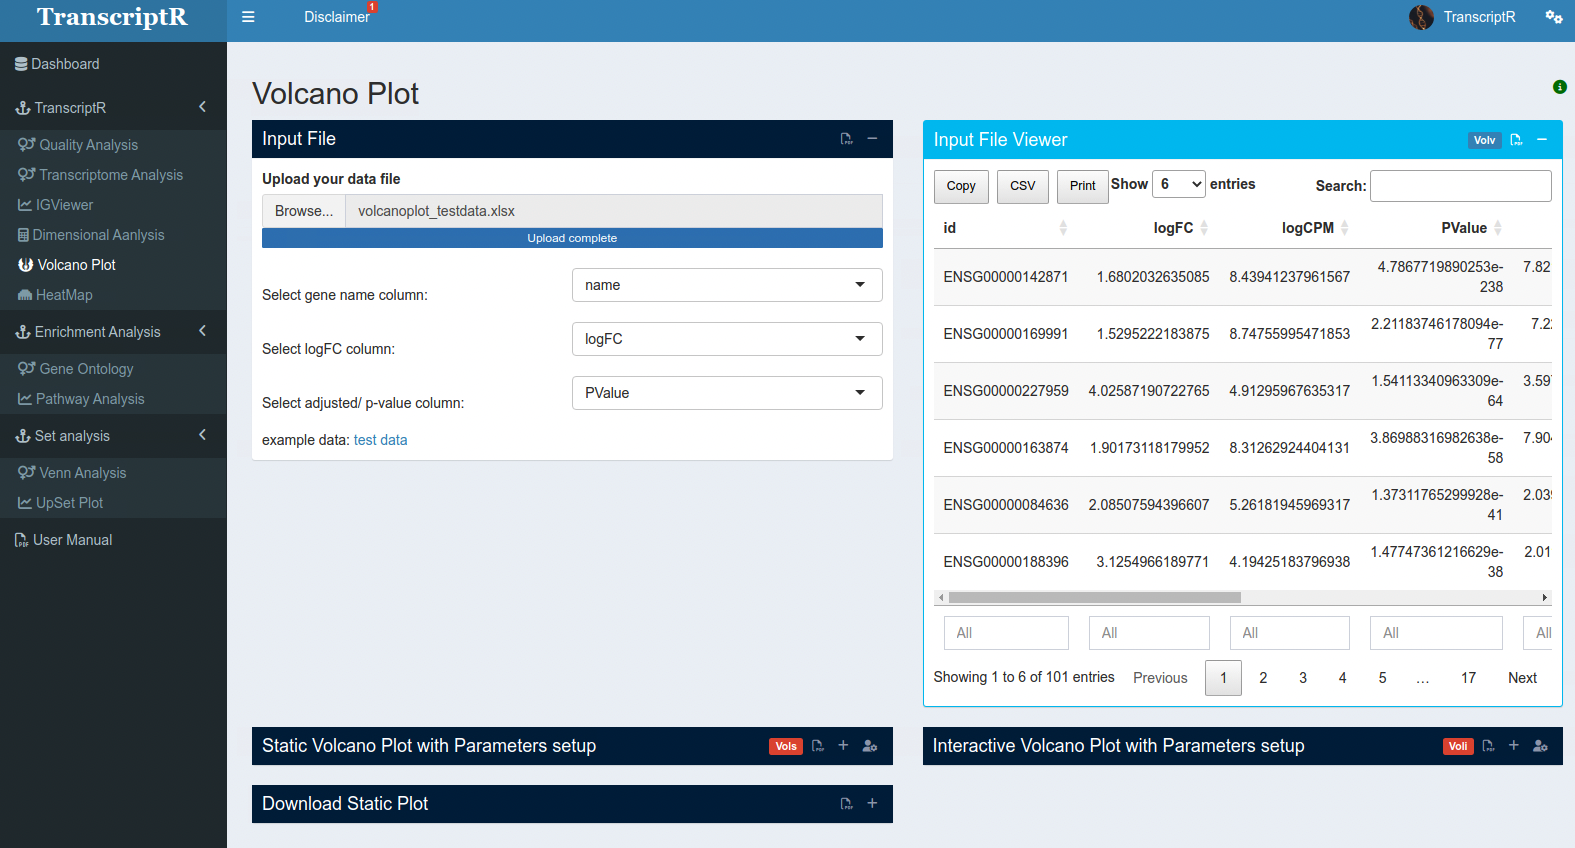
\includegraphics{images/volcano/volcano1.png}

}

\caption{\label{fig-vol1}Volcano: Infut file}

\end{figure}%

\subsection{Static Volcano Plot}\label{static-volcano-plot}

In this module, we introduced two versions of same volcano plot, static
and interactive volcano plot.

\begin{figure}[H]

\centering{

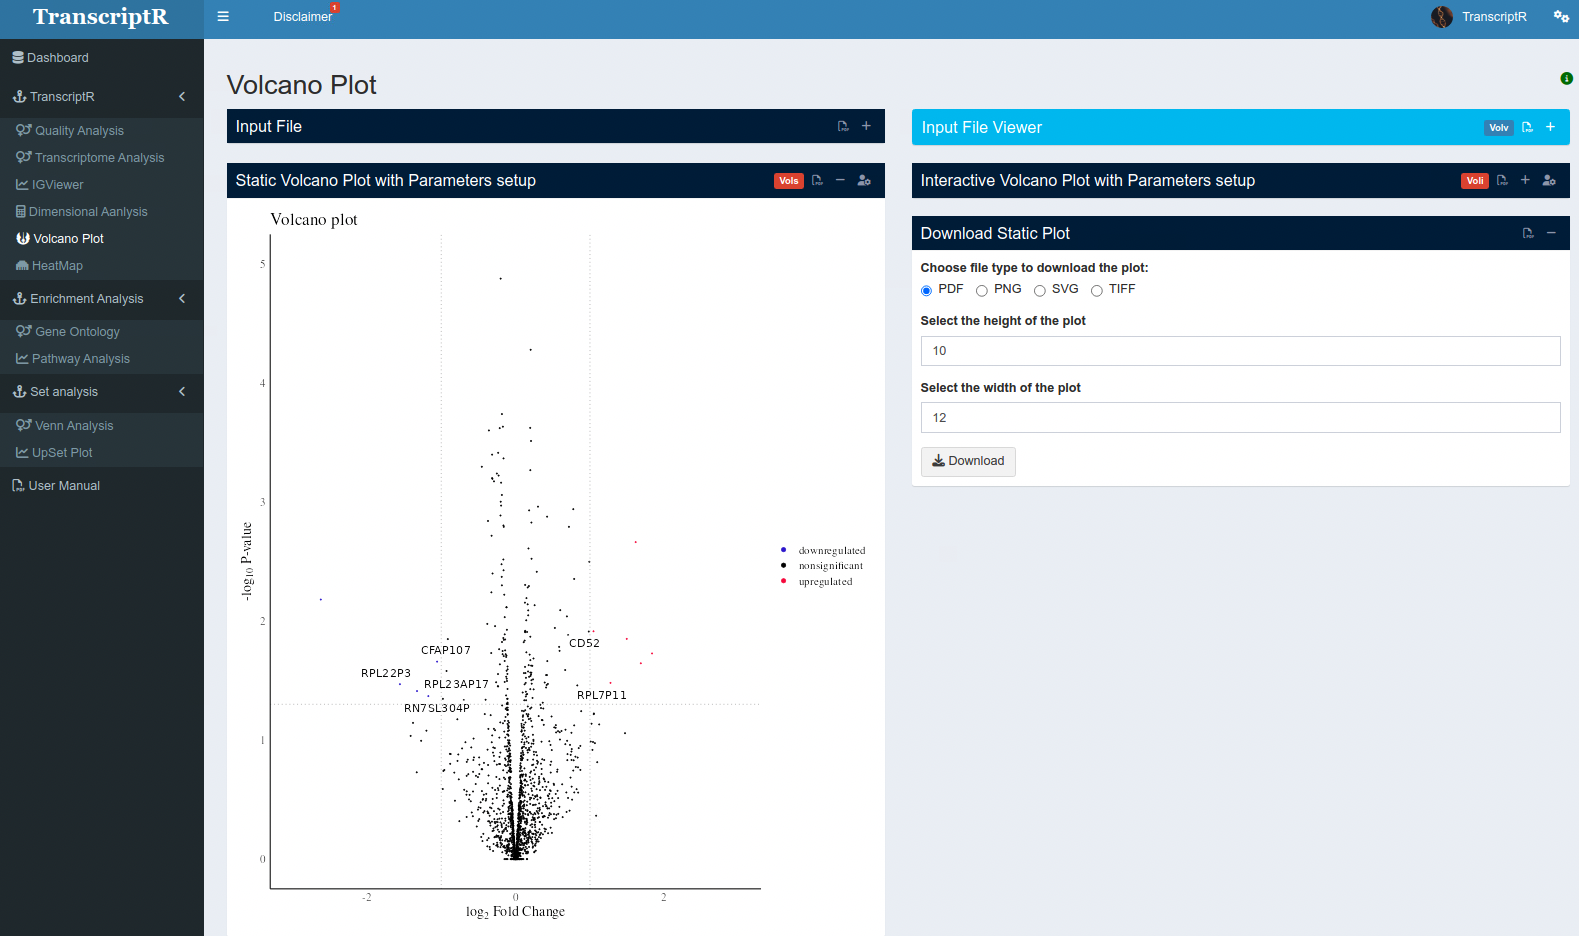
\includegraphics{images/volcano/volcano2.png}

}

\caption{\label{fig-volstat}Volcano plot}

\end{figure}%

\subsubsection{Parameters}\label{parameters}

\textbf{Main parameters}\\
1. \emph{Select number of genes to show}: User can select how many
genes/gene symbols they want to display. Default is 20. The plot will
display first 20 gene symbols on both upregulated and downregulated gene
symbols.\\
2. \emph{Change the genes font size}: Gene symbol font size can be
increased by increase this parameters for better visualization. Please
remember, if you want to show many gene symbols, increasing font size
may overlap the gene symbols.\\
3. \emph{Select cut-off for log2FC}: Users can apply a cut-off for
log2FC here. The default is 1.\\
4. \emph{Choose X-axis range}: X-axis range represents log2FC and user
can set the range for display. The default is -10 to 10.\\
5. \emph{Choose Y-axis range}: Y-axis range displays the p-value or
adjusted p-value (selected by the user in column 3, mentioned as above).
The default is 0 to 10.

\textbf{Change Colors}\\
6. \emph{Select color for downregulated}: User can select color for
downregulated genes.\\
7. \emph{Select color for upregulated}: User can select color for
upregualted genes.\\
8. \emph{Select color for non-significant}: User can select color for
non-significant genes (based on log2FC and p-value/adjusted p-value
cut-off).

\textbf{Change Font size, family and color}\\
9. \emph{Change the font size}: User can change the font size (other
parameters than gene symbol font size) of X- and Y- axes.\\
10. \emph{Select the font color}: User can change the font color (other
parameters than gene symbol font color) of X- and Y- axes.\\
11. \emph{Change the font family}: User can change the font family
(other parameters than gene symbol font family) of X- and Y- axes.

\textbf{Adjust lines}\\
12. \emph{Select color for log2FC cut-off line}: User can change the
color for the log2FC cut-off line.\\
13. \emph{Select color for p-value cut-off line}: User can change the
color for the p-value/adjusted p-value (as they choose in the option)
cut-off line.\\
14. \emph{Change the line type}: User can choose to select the line type
for both log2FC and p-value/adjusted p-value cut-off lines from the
drop-down list.

\textbf{Lables and titles}\\
15. \emph{X/Y-axis label}: We provided part of X abd Y-axis labels
(\textbf{\emph{log2/-log10}} as they are caclulated) and user can choose
to write their own labels for the axes. 16. \emph{Title}: User can write
their own title of the plot.

After the reuired changes in the parameter settings, user can click on
\emph{`Submit'} button and the plot will be displayed.

\subsection{Interactive Volcano plot with parameters
setup}\label{interactive-volcano-plot-with-parameters-setup}

For interactive volcano plot, we have provided two parameter settings -

\subsubsection{Parmeters settings}\label{parmeters-settings}

\begin{enumerate}
\def\labelenumi{\arabic{enumi}.}
\tightlist
\item
  \emph{Choose p-value/ adjusted p-value cut-off}: User can choose their
  own cut-off for p-value/adjusted p-value.
\item
  \emph{Choose log2FC cut-off}: User can choose their own cut-off for
  p-value/adjusted p-value.
\end{enumerate}

Click on \emph{`Run Analysis'} and the plot will be displayed after
calculation.

\section{Analysis result}\label{analysis-result-2}

The figure will generated as soon as the computation finishes. However,
it might takes some more time depending on the size of the file. If user
upload a file with 750K rows, it will take 3-5 minutes to generate the
figure (See Appendix~\ref{sec-calctime}). It is noteworthy that this big
data in volcano plot, may be unstable in the browser.

\subsection{Download static plot}\label{download-static-plot}

We addded multiple options to download the static volcano plot as can be
seen Figure~\ref{fig-volstat}. User can choose their own the file
format, size, resolution to download the file.

\subsection{Download interactive volcano
plot}\label{download-interactive-volcano-plot}

User can download the plot as figure (same as before) and the dynamic
figure as a html file.

\begin{tcolorbox}[enhanced jigsaw, coltitle=black, colback=white, title=\textcolor{quarto-callout-note-color}{\faInfo}\hspace{0.5em}{Note}, leftrule=.75mm, titlerule=0mm, colframe=quarto-callout-note-color-frame, toprule=.15mm, opacityback=0, arc=.35mm, breakable, rightrule=.15mm, colbacktitle=quarto-callout-note-color!10!white, bottomtitle=1mm, opacitybacktitle=0.6, left=2mm, bottomrule=.15mm, toptitle=1mm]

Please note displaying of the volcano plot will take some time, even
after the warning {``generating plot, please wait\ldots{}''}
\textcolor{orange}{"generating plot, please wait..."} disappears. Please
wait for 1-2 minutes to get the visualization.

\end{tcolorbox}

\begin{tcolorbox}[enhanced jigsaw, coltitle=black, colback=white, title=\textcolor{quarto-callout-tip-color}{\faLightbulb}\hspace{0.5em}{Tip}, leftrule=.75mm, titlerule=0mm, colframe=quarto-callout-tip-color-frame, toprule=.15mm, opacityback=0, arc=.35mm, breakable, rightrule=.15mm, colbacktitle=quarto-callout-tip-color!10!white, bottomtitle=1mm, opacitybacktitle=0.6, left=2mm, bottomrule=.15mm, toptitle=1mm]

Volcano plot figure colors annotation- {Significant \& Fold
Change}\textcolor{pink}{"Significant \& Fold Change"}, {Significant}
\textcolor{cyan}{"Significant"}, {FoldChange}
\textcolor{green}{FoldChange} or {NotSignificant}
\textcolor{orange}{"Notsignificant"}

\end{tcolorbox}

\section{R packages used}\label{r-packages-used-1}

\begin{enumerate}
\def\labelenumi{\arabic{enumi}.}
\tightlist
\item
  \href{}{EnhancedVolcano}
\item
  \href{https://cran.r-project.org/web/packages/plotly/plotly.pdf}{plotly}
\end{enumerate}

\chapter{HeatMap}\label{heatmap}

\part{Enrichment Analysis}

\chapter{Gene Ontology (GO) enrichment analysis}\label{sec-go}

\footnote{TO ALL OUR USERS, IF YOU ARE EXPERIENCING ANY TROUBLE WITH THE
  APP, BEFORE SENDING THE BUG REPORT, PLEASE RESTART THE DOCKER
  CONTAINER AND TRY AGAIN.}

Gene Ontology is a very well-known method for accessing the functions of
the gene identified through methylation analysis or expression analysis.
Here in \emph{TranscriptR}, we used ontology analysis using the
\href{https://bioconductor.org/packages/release/bioc/html/clusterProfiler.html}{clusterProfiler
package} \autocite{yu2012clusterprofiler,wu2021clusterprofiler}.

\section{How to use}\label{how-to-use-4}

\subsection{Data upload \& Parameters
setup}\label{data-upload-parameters-setup}

\subsubsection{Parameters setup}\label{parameters-setup}

\begin{enumerate}
\def\labelenumi{\arabic{enumi}.}
\tightlist
\item
  \emph{Choose GO analysis type}: user can choose to do the analysis
  whether \textbf{over-representation analysis} or the \textbf{gene-set
  enrichment analysis} (GSEA) from the drop-down menu.
\item
  \emph{Select the adjusted p-value}: user can also choose the adjusted
  \emph{p}-value for the analysis. Default is set to 0.05.
\item
  \emph{Select P-value adjustment method} As per clusterProfiler, we set
  different \emph{p}-value adjustment methods, Benjamini-Hochberg,
  Benjamini-Yeketuli, Bonferroni, Holm, Hommel, Hochberg, FDR or none.
  Default is Benjamini-Hochberg.
\item
  \emph{Select ontology class}: As defined in GO classification, we
  included all three ontology classes which user can select to show the
  plot.
\end{enumerate}

\subsubsection{Data upload}\label{data-upload-3}

At present, user can upload the DMC data produced by the main analysis
(see Chapter~\ref{sec-transcript} ) directly. The input file should be
in a \textbf{text (tab-delimited)} format.

\section{Analysis result}\label{analysis-result-3}

\begin{enumerate}
\def\labelenumi{\arabic{enumi}.}
\tightlist
\item
  On the right tab, the analysis result the plot will be generated as
  soon as computation finished. The plot is generated with plotly and it
  will be dynamic in nature as before. User can download the plot as PNG
  format, zoom in/out or do other stuffs as per plotly figures. The
  dynamic figure can also be downloaded as a html file.
\end{enumerate}

\begin{tcolorbox}[enhanced jigsaw, coltitle=black, colback=white, title=\textcolor{quarto-callout-note-color}{\faInfo}\hspace{0.5em}{Note}, leftrule=.75mm, titlerule=0mm, colframe=quarto-callout-note-color-frame, toprule=.15mm, opacityback=0, arc=.35mm, breakable, rightrule=.15mm, colbacktitle=quarto-callout-note-color!10!white, bottomtitle=1mm, opacitybacktitle=0.6, left=2mm, bottomrule=.15mm, toptitle=1mm]

\begin{enumerate}
\def\labelenumi{\arabic{enumi}.}
\tightlist
\item
  All horizontal bars (Gene Ontology terms) are clickable and will open
  a new tab with the respective gene onlogy detail from the
  \href{http://amigo.geneontology.org/amigo}{AmiGO} database.
\item
  Each interactive figure can be downloaded as HTML file and PNG file.
  The HTML file is clickable and each gene ontology term can open the
  respective detail from
  \href{http://amigo.geneontology.org/amigo}{AmiGO} database.
\end{enumerate}

\end{tcolorbox}

\subsection{Biological processes}\label{biological-processes}

\begin{figure}[H]

{\centering 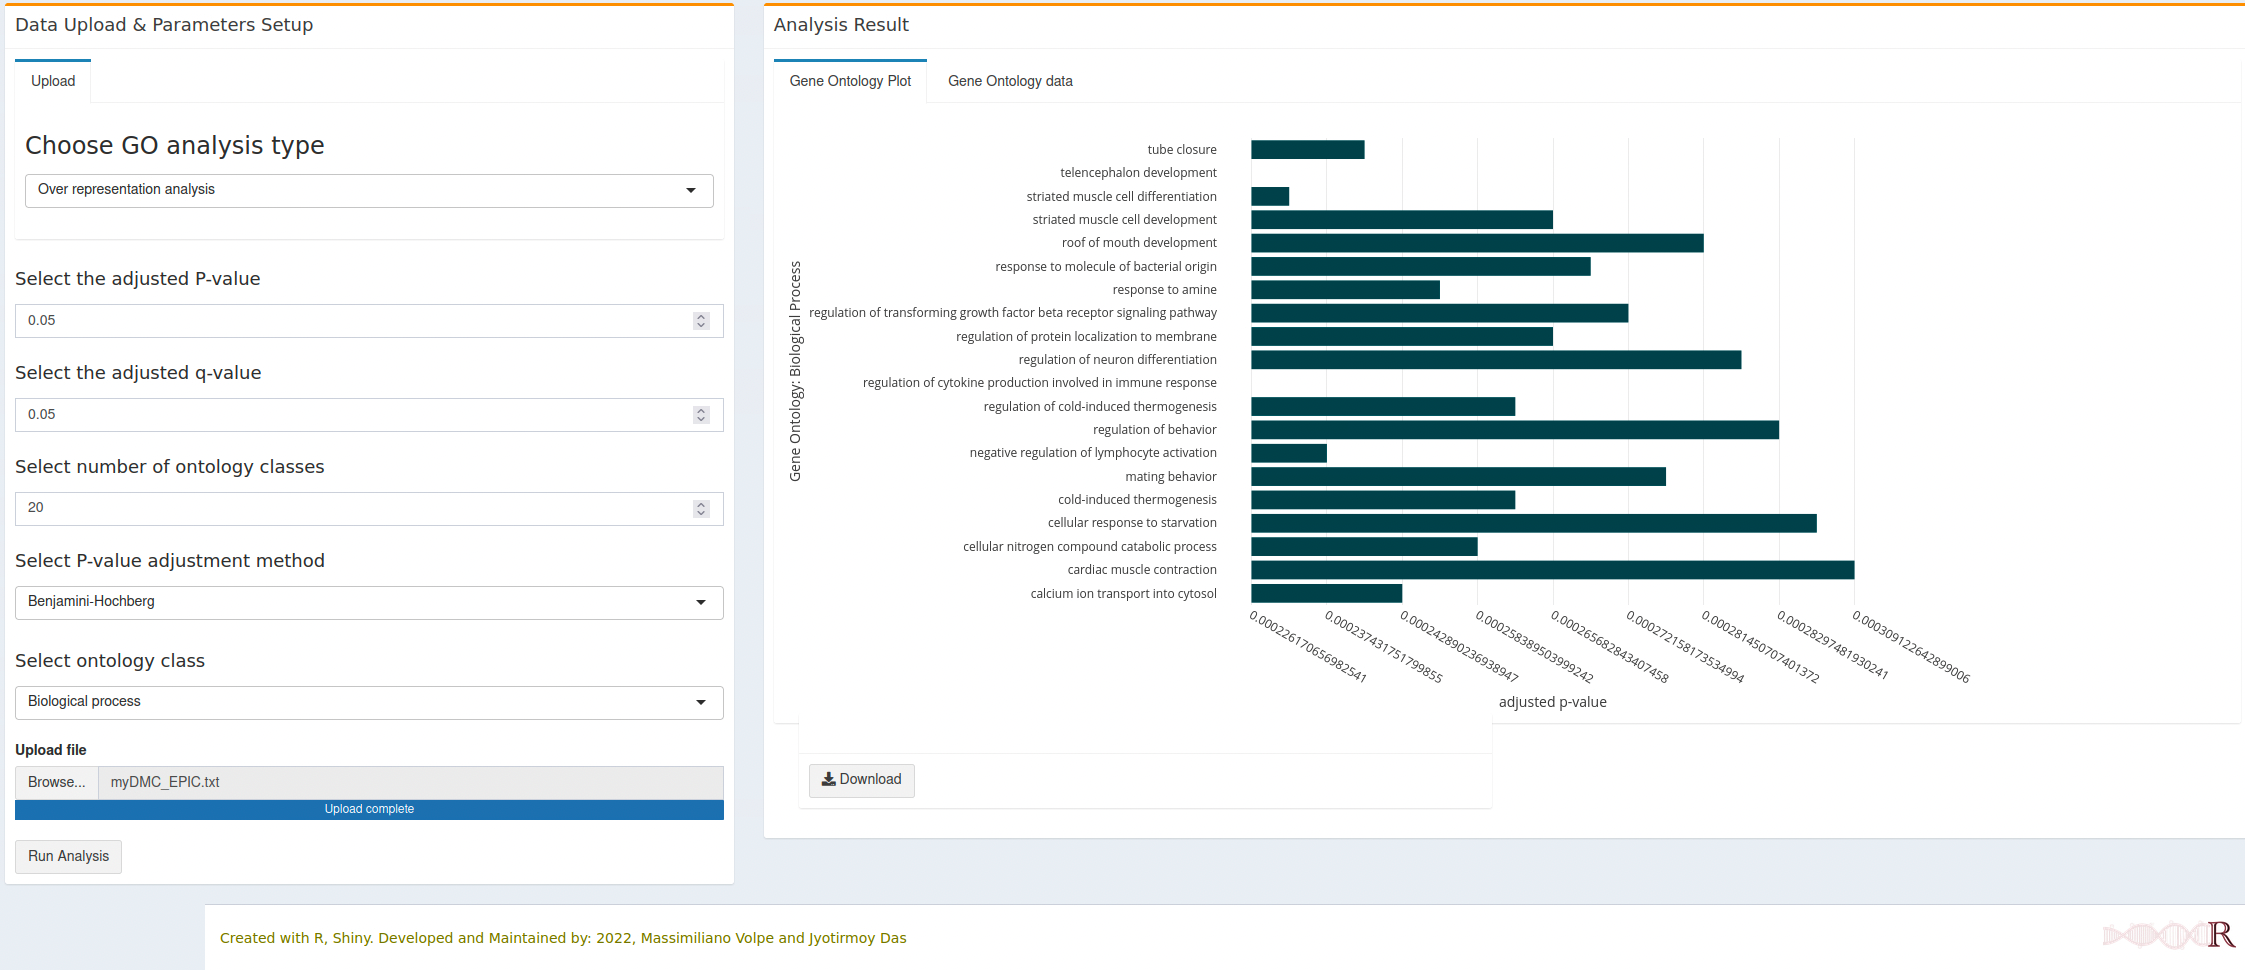
\includegraphics{images/GO-BP.png}

}

\caption{Gene Ontology - Biological Processes}

\end{figure}%

\subsection{Cellular component}\label{cellular-component}

\begin{figure}[H]

{\centering 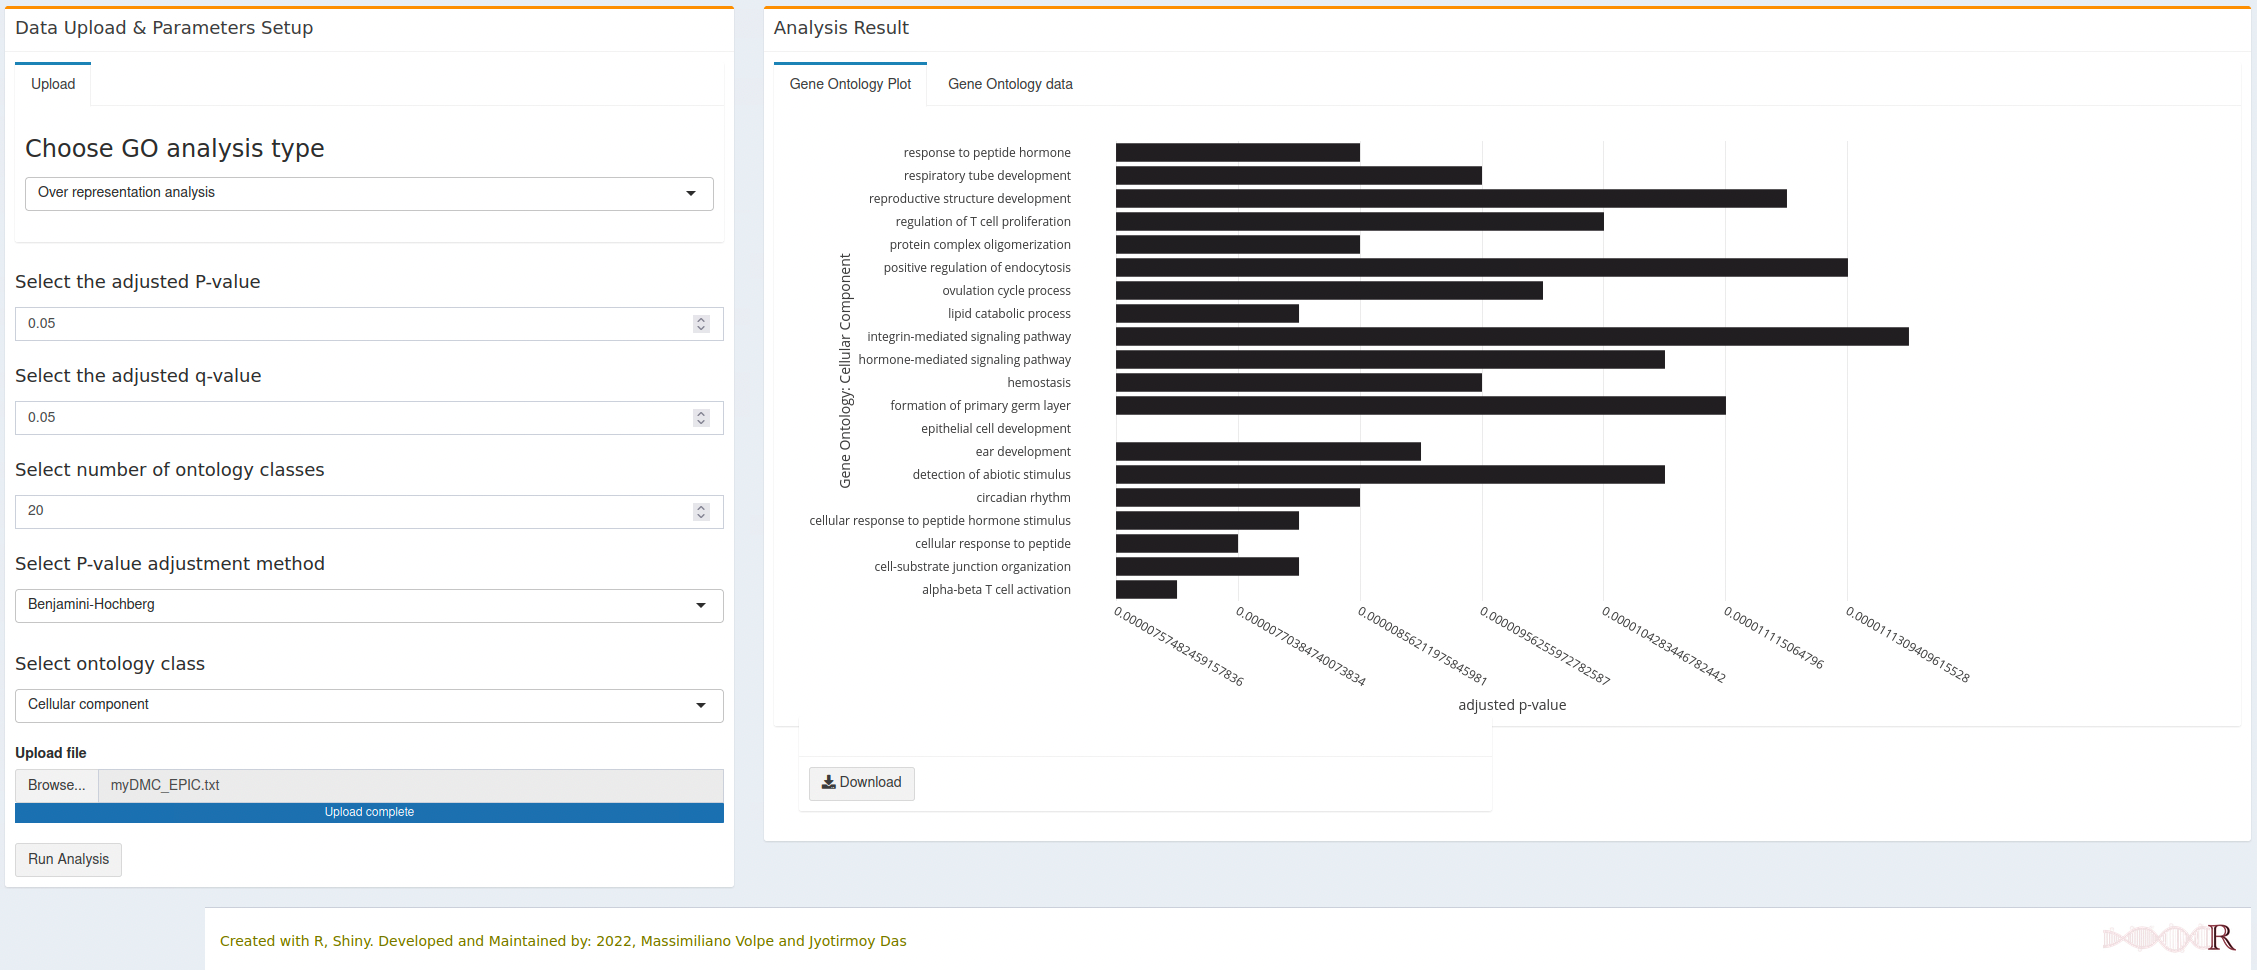
\includegraphics{images/GO-CC.png}

}

\caption{Gene Ontology - Cellular Component}

\end{figure}%

\subsection{Molecular function}\label{molecular-function}

\begin{figure}[H]

{\centering 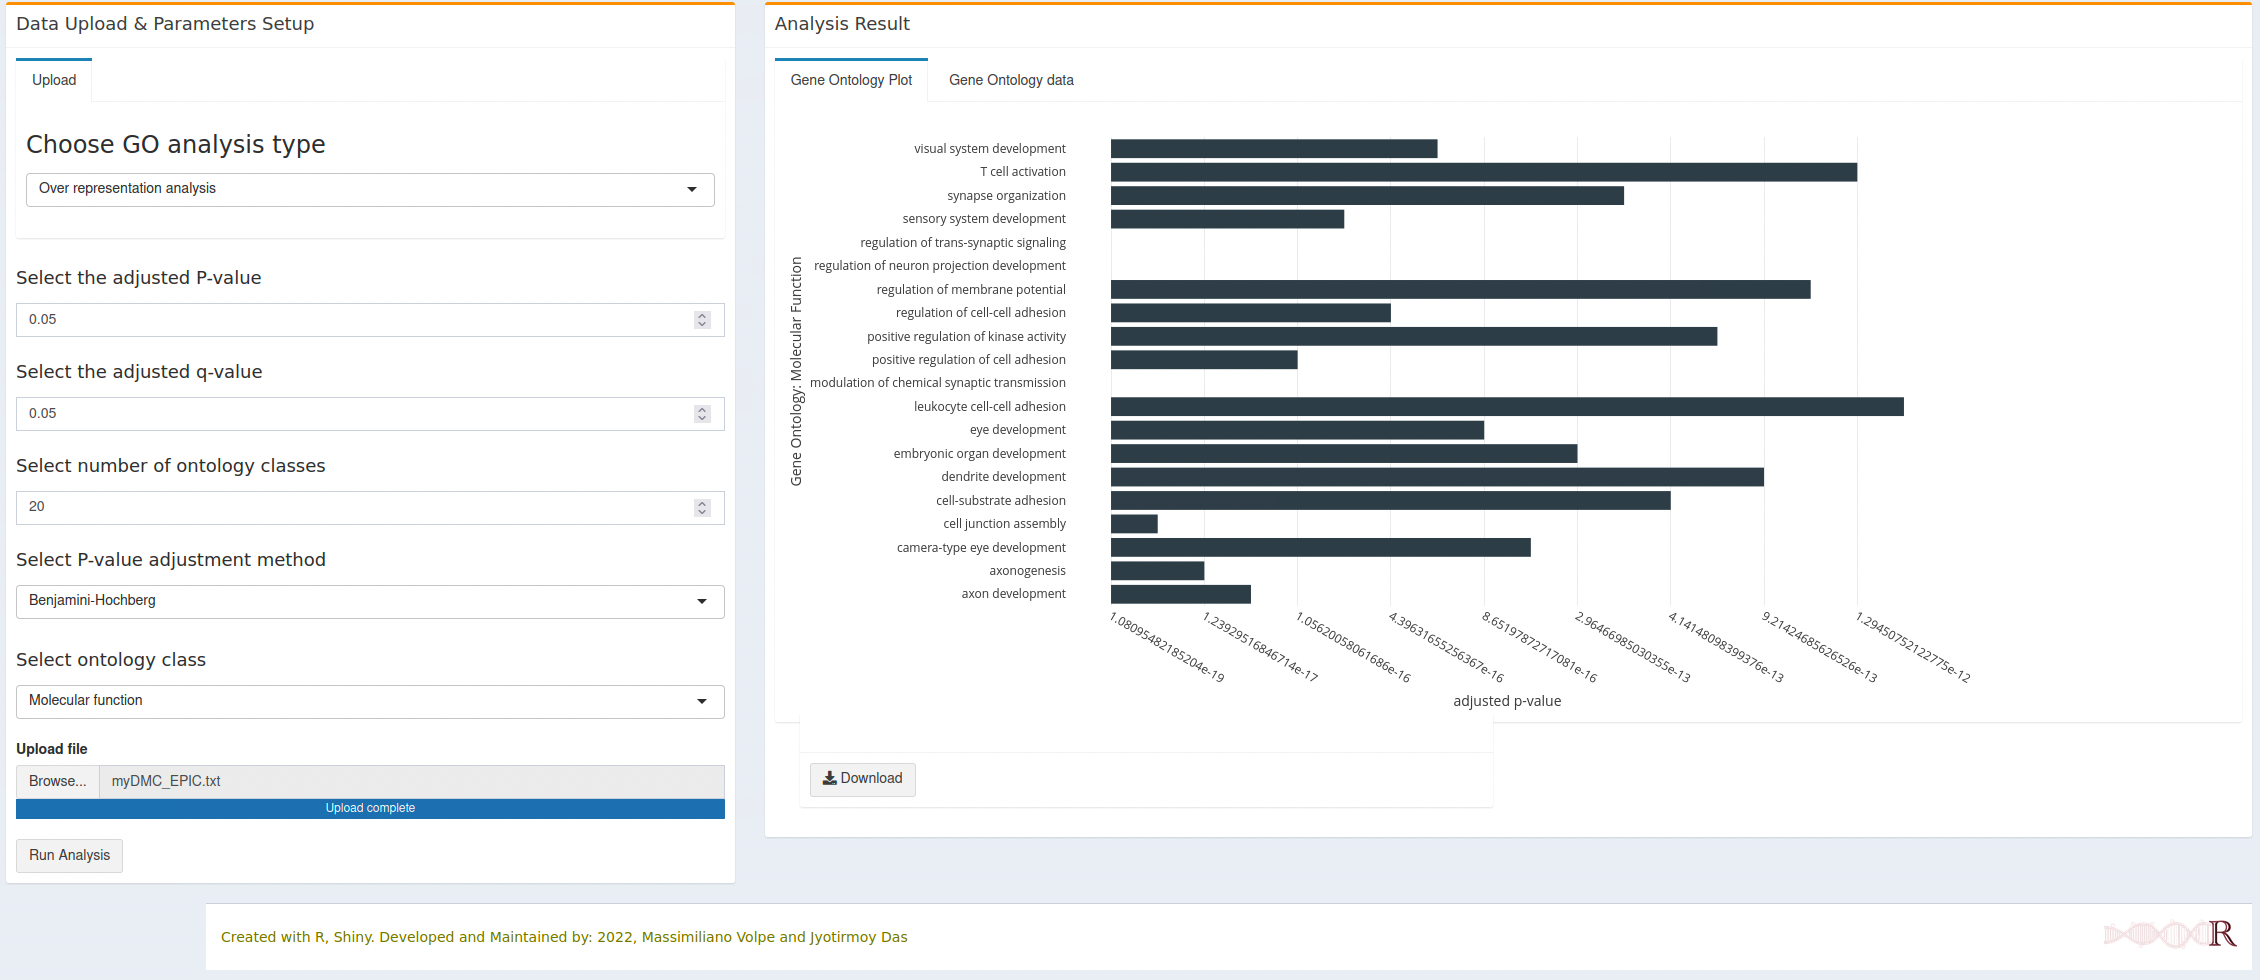
\includegraphics{images/GO-MF.png}

}

\caption{Gene Ontology - Molecular Function}

\end{figure}%

\begin{enumerate}
\def\labelenumi{\arabic{enumi}.}
\setcounter{enumi}{1}
\tightlist
\item
  On the second right tab, user will get the result as a table format.
  It might takes some time to compute result and generates the table.
  User can download the result as an Excel file from the current page or
  the entire result.\\
\end{enumerate}

\begin{figure}[H]

{\centering 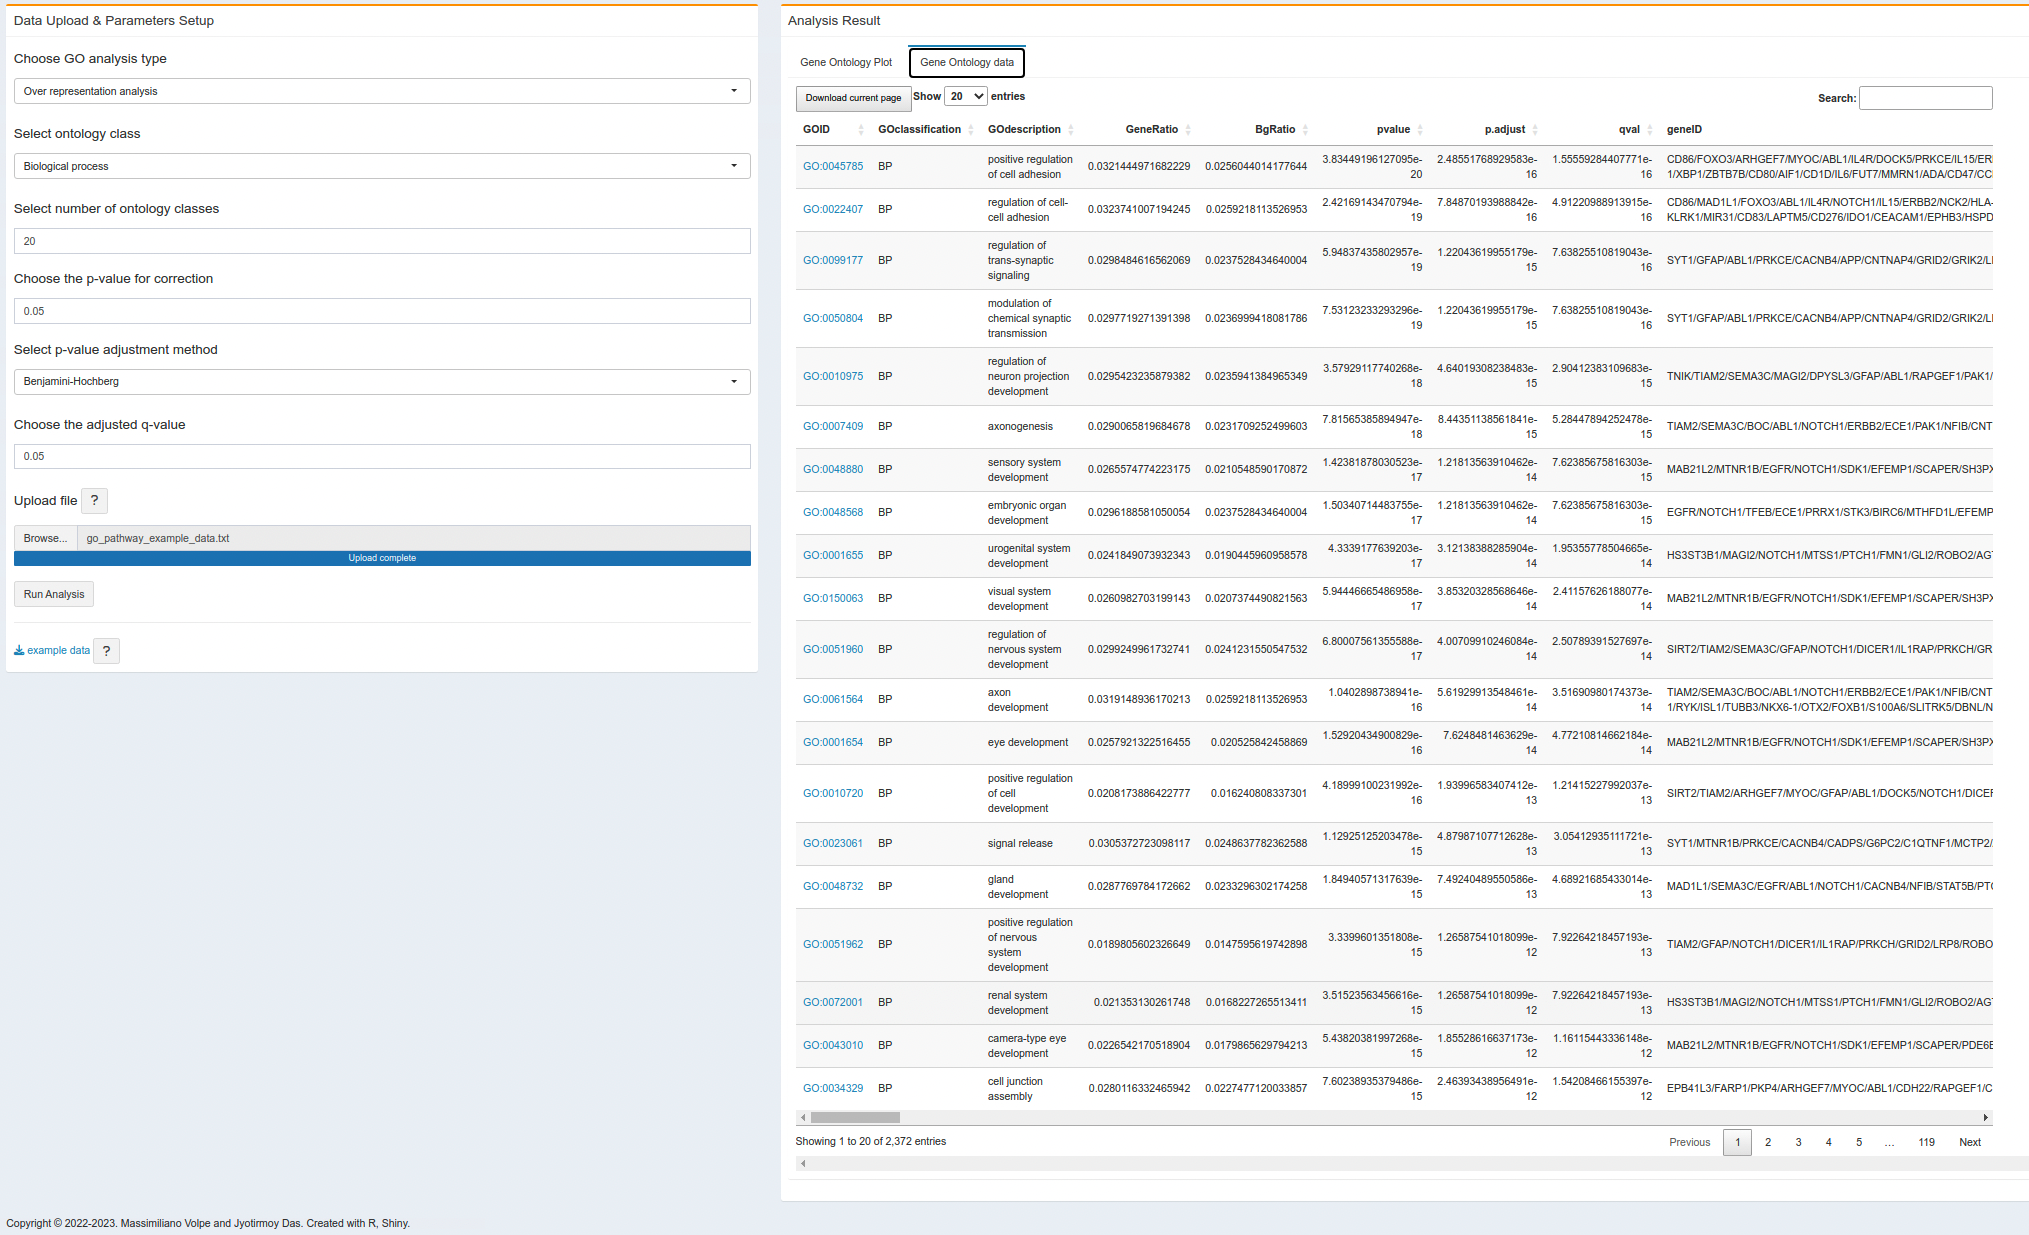
\includegraphics{images/GO-table.png}

}

\caption{Gene Ontology data table}

\end{figure}%

\begin{tcolorbox}[enhanced jigsaw, coltitle=black, colback=white, title=\textcolor{quarto-callout-warning-color}{\faExclamationTriangle}\hspace{0.5em}{Warning}, leftrule=.75mm, titlerule=0mm, colframe=quarto-callout-warning-color-frame, toprule=.15mm, opacityback=0, arc=.35mm, breakable, rightrule=.15mm, colbacktitle=quarto-callout-warning-color!10!white, bottomtitle=1mm, opacitybacktitle=0.6, left=2mm, bottomrule=.15mm, toptitle=1mm]

\begin{enumerate}
\def\labelenumi{\arabic{enumi}.}
\tightlist
\item
  In the gene onlogy enrichment table, the GO ID is clickable and will
  open the respective GO class from the AmiGO database. However, this
  feature is only avaible on the browser, if the user download the
  table, there is no such link to check the GO source.
\item
  The GO enrichment table will download the full result (i.e., all GO
  classes, Cellular Component, Molecular Function and Biological
  Processes), user donot need to run the table again for different GO
  classes.
\end{enumerate}

\end{tcolorbox}

\section{R packages used}\label{r-packages-used-2}

\begin{enumerate}
\def\labelenumi{\arabic{enumi}.}
\tightlist
\item
  \href{https://bioconductor.org/packages/release/bioc/vignettes/clusterProfiler/inst/doc/clusterProfiler.html}{clusterProfiler}
\end{enumerate}

\chapter{Pathway enrichment analysis}\label{sec-pathway}

\footnote{TO ALL OUR USERS, IF YOU ARE EXPERIENCING ANY TROUBLE WITH THE
  APP, BEFORE SENDING THE BUG REPORT, PLEASE RESTART THE DOCKER
  CONTAINER AND TRY AGAIN.}

Pathway enrichment analysis helps the user to get the mechanistic
insights of the important genes from genome-wide data analysis. In
\emph{TranscriptR}, we introduced the pathway analysis module that can
compute the enriched pathways from three different databases,
\href{https://www.genome.jp/kegg/}{KEGG} \autocite{Kanehisa2000},
\href{https://reactome.org/}{Reactome} \autocite{Gillespie2021} and
\href{https://www.wikipathways.org/}{Wikipathways}
\autocite{pico2008plos,martens2020nar}.

\section{How to use}\label{how-to-use-5}

\subsection{Data upload \& Parameters
setup}\label{data-upload-parameters-setup-1}

\begin{enumerate}
\def\labelenumi{\arabic{enumi}.}
\item
  \textbf{Select Database} User needs to select the database from the
  drop-down list (\href{https://www.genome.jp/kegg/}{KEGG},
  \href{https://reactome.org/}{Reactome},
  \href{https://www.wikipathways.org/}{Wikipathways}) for the analysis.
  Default is \textbf{KEGG database}
\item
  \textbf{Select Organism} In the next step, please select the organism
  from the drop-down list. The default sets to \textbf{`Homo sapiens
  (Human)'}.
\end{enumerate}

\begin{tcolorbox}[enhanced jigsaw, coltitle=black, colback=white, title=\textcolor{quarto-callout-important-color}{\faExclamation}\hspace{0.5em}{Important}, leftrule=.75mm, titlerule=0mm, colframe=quarto-callout-important-color-frame, toprule=.15mm, opacityback=0, arc=.35mm, breakable, rightrule=.15mm, colbacktitle=quarto-callout-important-color!10!white, bottomtitle=1mm, opacitybacktitle=0.6, left=2mm, bottomrule=.15mm, toptitle=1mm]

Please note that for the three different databases (KEGG, Reactome and
Wikipathways), we have different sets of organisms. In KEGG, the list is
added from KEGG databases \emph{(only mammals)}, other databases are
showing organisms based on the availability in bioconductor.

\end{tcolorbox}

\begin{enumerate}
\def\labelenumi{\arabic{enumi}.}
\setcounter{enumi}{2}
\item
  \textbf{Select analysis type} Choose the type of pathway enrichment
  analysis from the drop-down list, \emph{Over-representation} or
  \emph{GeneSet Enrichment Analysis (GSEA)}. The default is
  \textbf{over-representation}.
\item
  \textbf{Select P-value cut-off for correction} The default value for
  \emph{p}-value correction is set to 0.05. User can set their own
  cut-off values.
\item
  \textbf{Select P-value correction method} The default method for
  adjustment of P-value is the Benjamini-Hochberg (BH) correction
  method. User can choose different method using the drop-down list:

  \begin{itemize}
  \tightlist
  \item
    Benjamini-Hochberg (BH)
  \item
    Benjamini-Yeketuli (BY)
  \item
    Bonferroni
  \item
    Holm
  \item
    Hommel
  \item
    Hochberg
  \item
    FDR
  \item
    none
  \end{itemize}
\item
  \textbf{Upload data file} User can upload/drag-and-drop the direct
  output result from the main analysis. The supported file formats are,
  excel (.xls, .xlsx), comma-separated (.csv) or tab-delimited (.txt).
  The uploaded file should have the header/column name.
\item
  \textbf{Select logFC/Gene name column} After the file upload, user
  needs to select the logFC and gene name (gene symbol) column (column
  name can be anything).
\item
  \textbf{Viewer panel and Run Analysis} Please check your upload file
  in the viewer panel and select the right columns for logFC and gene
  name/symbol.
\end{enumerate}

\begin{figure}[H]

\centering{

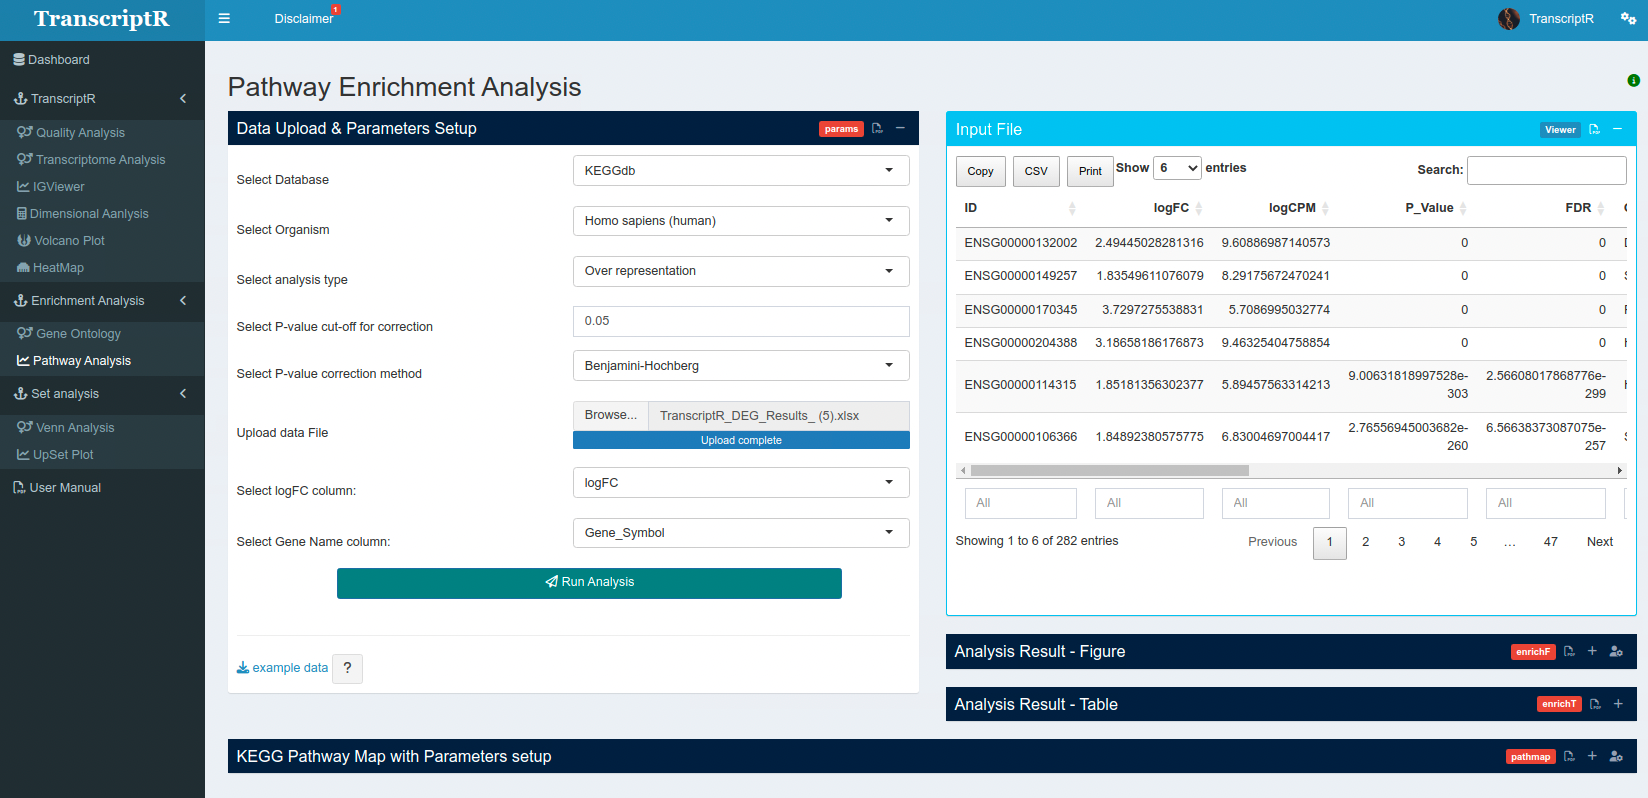
\includegraphics{images/pathway/path1.png}

}

\caption{\label{fig-path1}Input files and view}

\end{figure}%

\subsection{Analysis Result}\label{analysis-result-4}

In the \textbf{Analysis Result}, there are two parts,\\
- Figure\\
- Table

The Figure and Table is interactive.

\textbf{Figure parameters} We added few parameters in the
\textbf{Figure} (see Figure~\ref{fig-path11}) -

\begin{enumerate}
\def\labelenumi{\arabic{enumi}.}
\item
  \emph{Types of figure}: User can choose between 1) Scatter plot/dot
  plot and 2) bar plot. The default is \emph{dot plot}.
\item
  \emph{Color for high/mid/low p-value}: Colors for high (default is
  blue), mid (dafault is white), low (default is red) can be changed.
\item
  \emph{Titles}: User can write the title and x-/y-axis labels of the
  figure.
\end{enumerate}

\begin{figure}[H]

\centering{

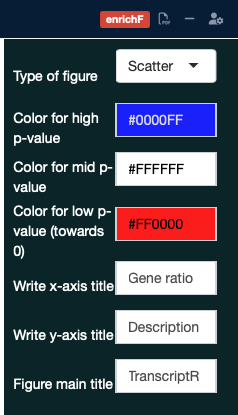
\includegraphics{images/pathway/path1-1.png}

}

\caption{\label{fig-path11}Figure parameters}

\end{figure}%

\textbf{Table} The table will display all results by pages. The user can
download the whole result table as an Excel file. If the user want to
select one/few enriched pathways (as dot on the plot), the table will be
updated interactively with the selected list (see
Figure~\ref{fig-path12}).

\begin{figure}[H]

\centering{

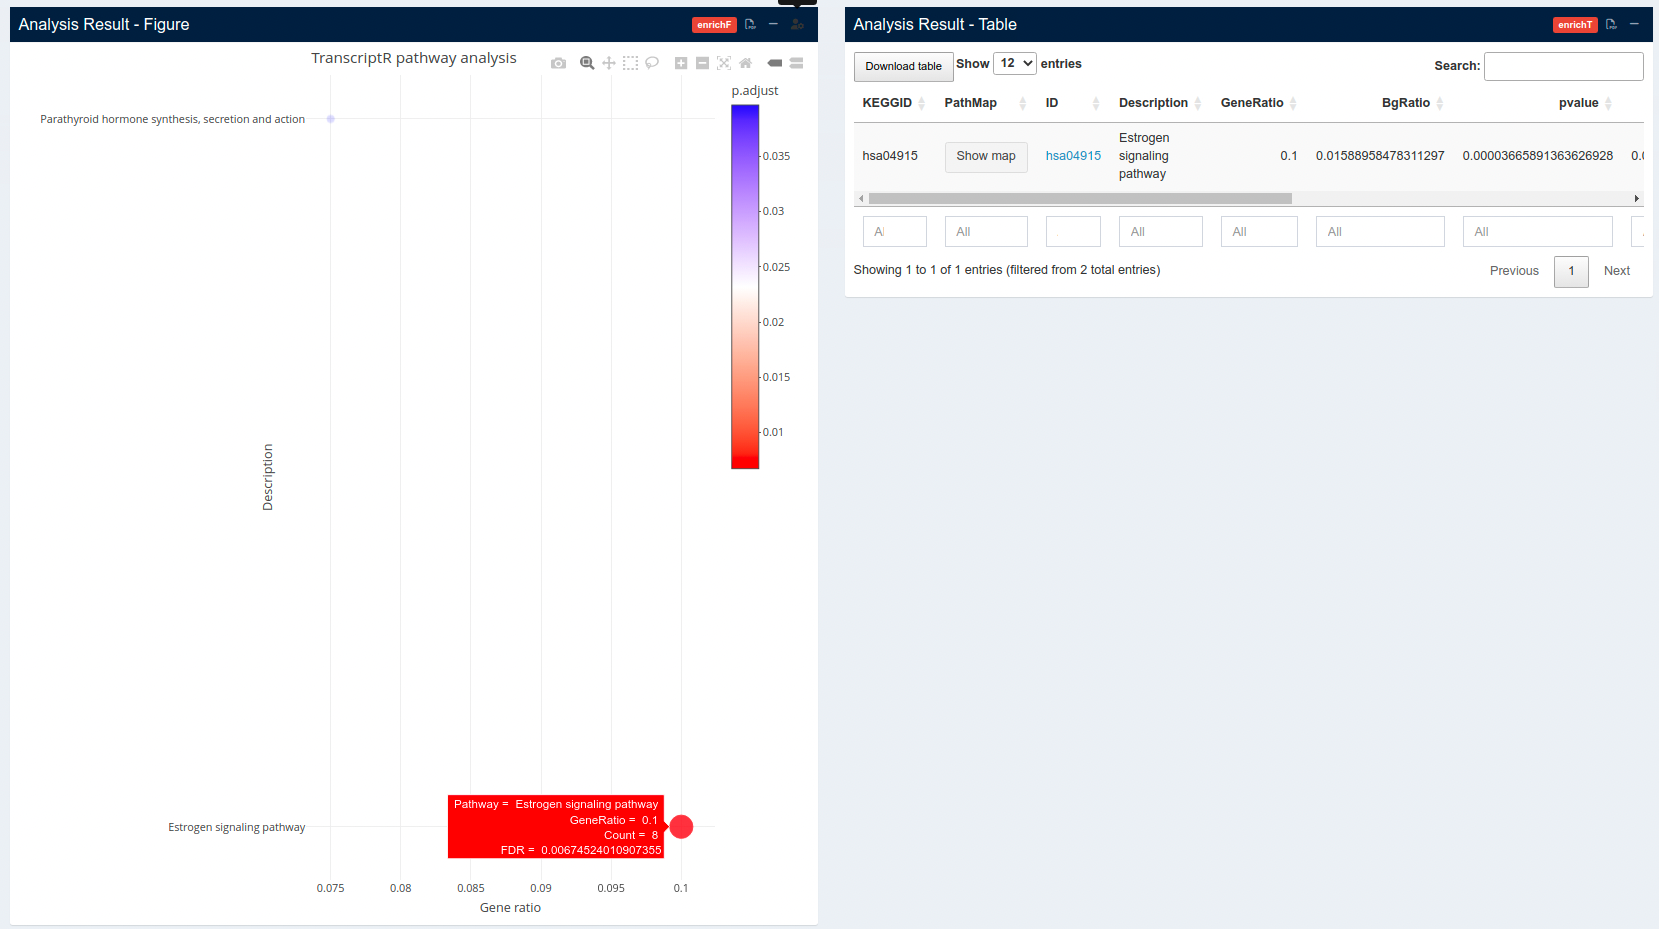
\includegraphics{images/pathway/path1-2.png}

}

\caption{\label{fig-path12}Analysis Result-interactivity}

\end{figure}%

In the table, we added following information -

\begin{itemize}
\tightlist
\item
  KEGGID
\item
  \emph{PathMap}: only available to KEGG database analysis result.
\item
  ID
\item
  Description
\item
  GeneRatio
\item
  BgRatio
\item
  pvalue
\item
  p.adjust
\item
  qval
\item
  geneID
\item
  Count
\end{itemize}

\textbf{KEGG Pathway Map with Parameters setup}

\begin{tcolorbox}[enhanced jigsaw, coltitle=black, colback=white, title=\textcolor{quarto-callout-important-color}{\faExclamation}\hspace{0.5em}{Important}, leftrule=.75mm, titlerule=0mm, colframe=quarto-callout-important-color-frame, toprule=.15mm, opacityback=0, arc=.35mm, breakable, rightrule=.15mm, colbacktitle=quarto-callout-important-color!10!white, bottomtitle=1mm, opacitybacktitle=0.6, left=2mm, bottomrule=.15mm, toptitle=1mm]

This feature only available to KEGG pathways.

\end{tcolorbox}

If the user selected \textbf{`KEGG database'} for the analysis, then the
result table will contain a column named \emph{PathMap} which displays
`show map' option against each enriched pathway. Once clicked on the
`show map' will trigger the result, \emph{KEGG pathway map with
parameters setup} (see Figure~\ref{fig-path12}).

\begin{figure}[H]

\centering{

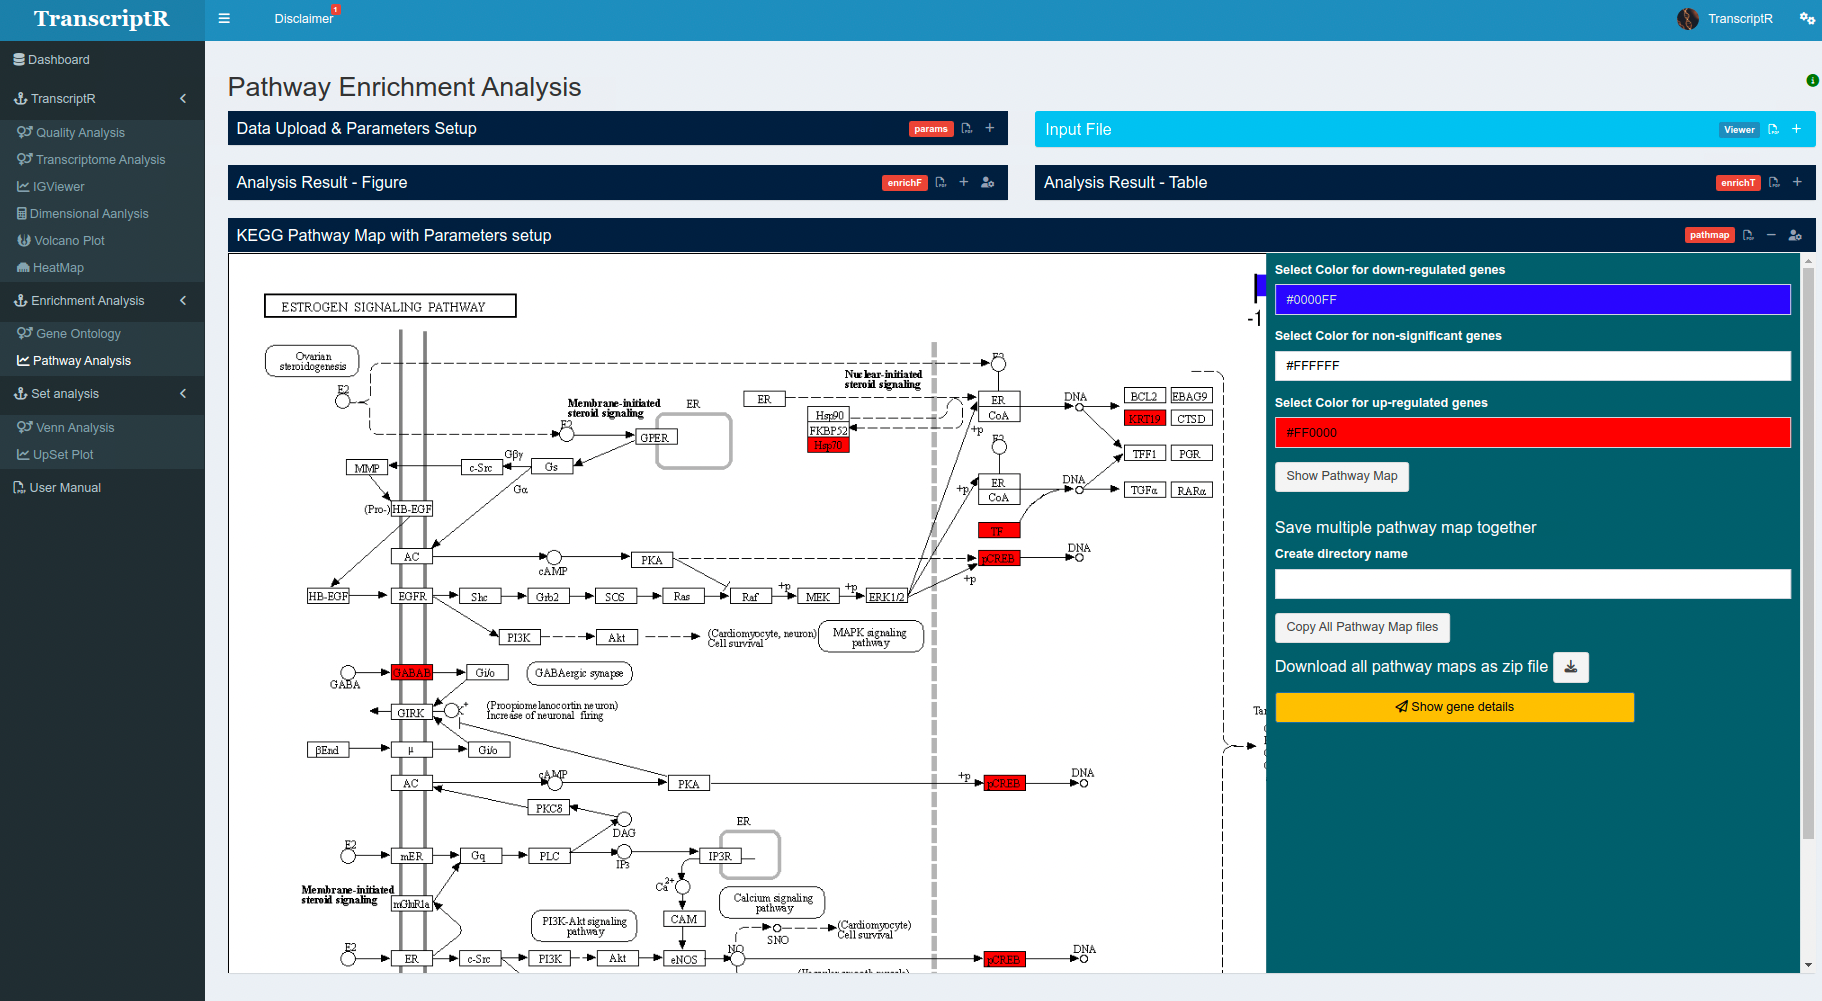
\includegraphics{images/pathway/path3.png}

}

\caption{\label{fig-path3}Pathway map}

\end{figure}%

\begin{itemize}
\item
  In this map, user can choose their own colors for up, down or
  non-significant genes in the pathway map (see Figure~\ref{fig-path3}).
\item
  PLEASE NOTE, if there is no map showed in the viewer panel, run
  \emph{Show Pathway Map} (see Figure~\ref{fig-path3}).
\item
  If the user wants multiple pathway map, they can choose to save in one
  folder and downloda all together. They can write their own folder name
  and download as zip (see Figure~\ref{fig-path3}).
\item
  Again, we added an option to see the `gene details' as this was not
  shown on the previous table (see Figure~\ref{fig-path4}).
\end{itemize}

\begin{figure}[H]

\centering{

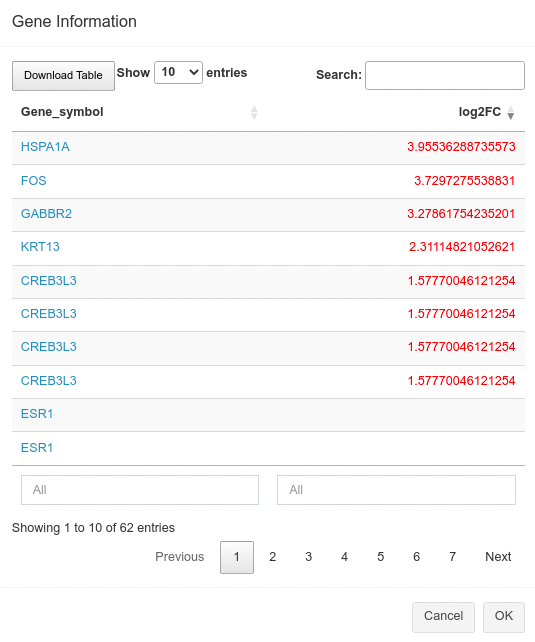
\includegraphics{images/pathway/path4.png}

}

\caption{\label{fig-path4}Gene details}

\end{figure}%

\begin{tcolorbox}[enhanced jigsaw, coltitle=black, colback=white, title=\textcolor{quarto-callout-note-color}{\faInfo}\hspace{0.5em}{Note}, leftrule=.75mm, titlerule=0mm, colframe=quarto-callout-note-color-frame, toprule=.15mm, opacityback=0, arc=.35mm, breakable, rightrule=.15mm, colbacktitle=quarto-callout-note-color!10!white, bottomtitle=1mm, opacitybacktitle=0.6, left=2mm, bottomrule=.15mm, toptitle=1mm]

\begin{enumerate}
\def\labelenumi{\arabic{enumi}.}
\item
  \emph{Pathway enrichment plot}: after ``Run Analysis'', the plot will
  be generated as soon as computation has been done. Depends on the size
  of data, it might take few minutes (See Appendix~\ref{sec-calctime}).
  The plot is interactive and with the mouse hovering, each dot/bar will
  show the pathway name, count of genes from the input list for that
  particular pathway, the corrected \emph{p}-value and gene ratio. The
  color scale bar shows in the legend. User can download the figure as
  PNG as described above and the interactive figure as a html file. The
  downloaded HTML file is clickable and each pathway enrichment term can
  open the respective database for pathway details.\\
\item
  All dots (pathway enrichment terms) are clickable and will open a new
  tab with the respective pathway detail from the selected database
  (Reactome/KEGG/Wiki).
\end{enumerate}

\end{tcolorbox}

\begin{tcolorbox}[enhanced jigsaw, coltitle=black, colback=white, title=\textcolor{quarto-callout-warning-color}{\faExclamationTriangle}\hspace{0.5em}{Warning}, leftrule=.75mm, titlerule=0mm, colframe=quarto-callout-warning-color-frame, toprule=.15mm, opacityback=0, arc=.35mm, breakable, rightrule=.15mm, colbacktitle=quarto-callout-warning-color!10!white, bottomtitle=1mm, opacitybacktitle=0.6, left=2mm, bottomrule=.15mm, toptitle=1mm]

In the pathway enrichment table, the pathway ID is clickable and will
open the respective pathway from the database. However, this feature is
only avaible on the browser, if the user download the table, there is no
such link to check the pathway source.

\end{tcolorbox}

\section{R packages used}\label{r-packages-used-3}

\begin{enumerate}
\def\labelenumi{\arabic{enumi}.}
\tightlist
\item
  \href{https://bioconductor.org/packages/release/bioc/vignettes/clusterProfiler/inst/doc/clusterProfiler.html}{clusterProfiler}
\end{enumerate}

\part{Set Analysis}

\chapter{Venn analysis}\label{sec-venn}

\footnote{TO ALL OUR USERS, IF YOU ARE EXPERIENCING ANY TROUBLE WITH THE
  APP, BEFORE SENDING THE BUG REPORT, PLEASE RESTART THE DOCKER
  CONTAINER AND TRY AGAIN.}

Venn analysis can be performed to show the logical relation between
sets. In this module, user will need two or more analyses (max 6
datasets) to perform the Venn analysis. We adopt the part from
\href{https://github.com/asntech/intervene}{intervene}
\autocite{khan2017intervene} application and modified as required for
\emph{methylR} use.

\section{How to use}\label{how-to-use-6}

Below given the details for the use of Venn analysis module.

\subsection{Data upload \& Parameters
setup}\label{data-upload-parameters-setup-2}

\subsubsection{Parameters setup}\label{parameters-setup-1}

\begin{enumerate}
\def\labelenumi{\arabic{enumi}.}
\item
  \emph{Upload}: Data can be uploaded as \textbf{Tab} (.txt) or
  \textbf{Comma} (.csv) or \textbf{Semicolon} (.csv but with ;)
  separated format. A demo test dataset is running by default and it is
  available for download by clicking on the ``example data'' button.
\item
  \emph{Settings}: Under settings, there are multiple options to display
  the plot -

  \begin{enumerate}
  \def\labelenumii{\roman{enumii}.}
  \tightlist
  \item
    \emph{Select sets}: will select sets from the uploaded data. User
    can remove the set as they need.
  \item
    \emph{Venn type}: different type of venn diagram can be selected
    from the drop-down menu
  \end{enumerate}

  \begin{itemize}
  \tightlist
  \item
    Chow-Ruskey
  \item
    Classical
  \item
    Edwards
  \item
    Square
  \item
    Battle
  \end{itemize}

  The diagram can be \emph{weighted} or \emph{Eular}.

  \begin{enumerate}
  \def\labelenumii{\roman{enumii}.}
  \setcounter{enumii}{2}
  \item
    \emph{Border line width}: border line can be drawn with the slider
    option.
  \item
    \emph{Border line type}: border line type can be selected from the
    drop-down menu.
  \item
    \emph{Zoom in/out Venn diagram}: select the zoom option on the slide
    bar.
  \end{enumerate}
\item
  \emph{Font \& Color}: multiple ooptions are included for font and
  colours -

  \begin{enumerate}
  \def\labelenumii{\roman{enumii}.}
  \item
    \emph{Select color theme}: Colour theme can be chosen from the
    drop-down menu.
  \item
    \emph{Label font size}: Change the font size of the Label.
  \item
    \emph{Number font size}: Change the font size of the number.
  \end{enumerate}
\end{enumerate}

\section{Results}\label{results}

User can download the figure in different format, PDF, PNG, SVG or TIFF.

\begin{figure}[H]

{\centering 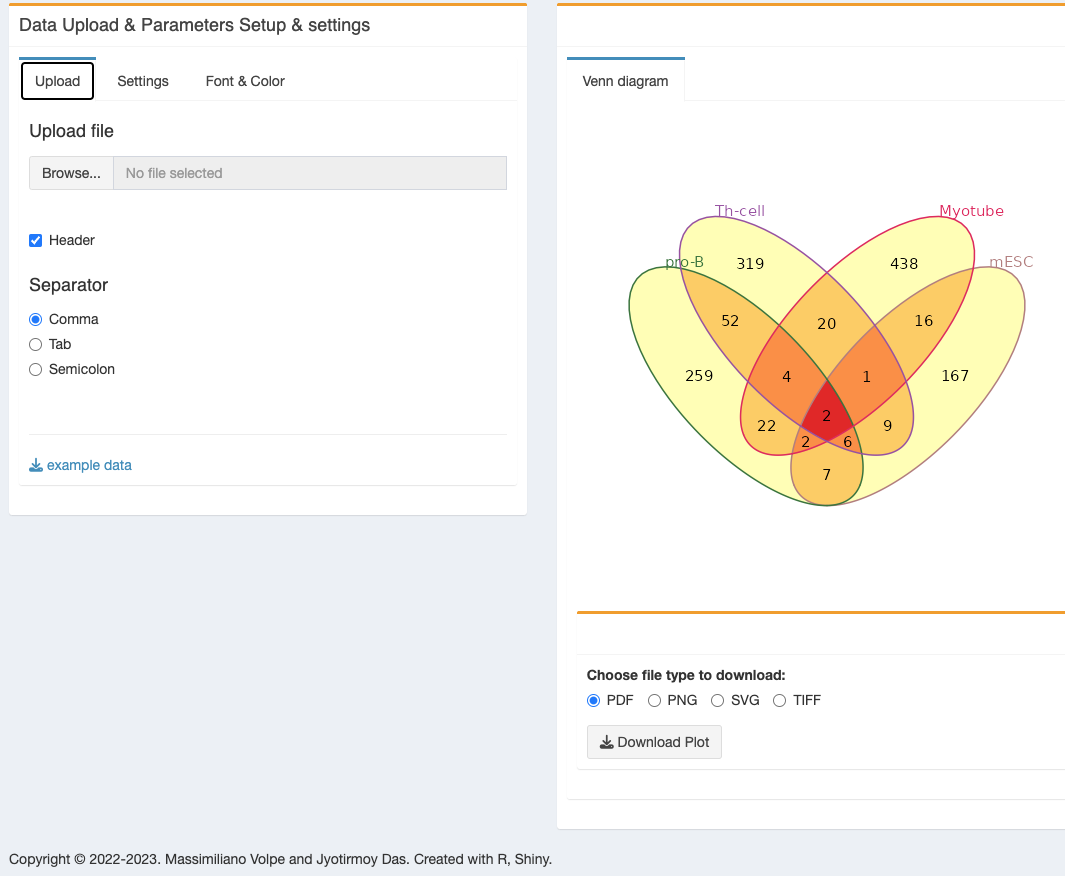
\includegraphics{images/Venndiag.png}

}

\caption{Venn Result}

\end{figure}%

\section{R packages used}\label{r-packages-used-4}

\begin{enumerate}
\def\labelenumi{\arabic{enumi}.}
\tightlist
\item
  \href{https://github.com/js229/Vennerable}{Vennerable}
\item
  \href{https://cran.r-project.org/web/packages/readr/readr.pdf}{readr}
\item
  \href{https://github.com/asntech/intervene}{intervene}
\end{enumerate}

\chapter{UpSet Plots}\label{sec-upset}

\footnote{TO ALL OUR USERS, IF YOU ARE EXPERIENCING ANY TROUBLE WITH THE
  APP, BEFORE SENDING THE BUG REPORT, PLEASE RESTART THE DOCKER
  CONTAINER AND TRY AGAIN.}

UpSet plot will show the relation between different sets. We adopt the
part from \href{https://github.com/asntech/intervene}{intervene}
\autocite{khan2017intervene} application and modified as required for
\emph{methylR} use.

\section{How to use}\label{how-to-use-7}

\subsection{Data upload}\label{data-upload-4}

\begin{enumerate}
\def\labelenumi{\arabic{enumi}.}
\item
  \emph{Upload}: Data can be uploaded as \textbf{Tab} (.txt) or
  \textbf{Comma} (.csv) or \textbf{Semicolon} (.csv but with ;)
  separated format. Please look into the example data file. A demo test
  dataset is running by default and it is available for download by
  clicking on the ``List example data'' button. UpSet module takes three
  types of inputs.

  \begin{enumerate}
  \def\labelenumii{\roman{enumii}.}
  \tightlist
  \item
    \emph{List type data}: List data is a correctly formatted csv/text
    file, with lists of names. Each column represents a set, and each
    row represents an element (names/gene/SNPs). Header names (first
    row) will be used as set names.
  \item
    \emph{Binary type data}: In the binary input file each column
    represents a set, and each row represents an element. If a names is
    in the set then it is represented as a 1, else it is represented as
    a 0.
  \item
    \emph{Combination/expression type data:} Combination/expression type
    data is the possible combinations of set intersections.
  \end{enumerate}
\end{enumerate}

\begin{tcolorbox}[enhanced jigsaw, coltitle=black, colback=white, title=\textcolor{quarto-callout-note-color}{\faInfo}\hspace{0.5em}{Note}, leftrule=.75mm, titlerule=0mm, colframe=quarto-callout-note-color-frame, toprule=.15mm, opacityback=0, arc=.35mm, breakable, rightrule=.15mm, colbacktitle=quarto-callout-note-color!10!white, bottomtitle=1mm, opacitybacktitle=0.6, left=2mm, bottomrule=.15mm, toptitle=1mm]

PLEASE NOTE: \textbf{\emph{``OR enter set combinations/expression''}}
has the priority over \textbf{``Upload file''}. If you use the ``set
combinations'', and then want to ``upload file'', please remove the
``set combination'' from the input box. To see how the ``OR enter set
combinations/expression'' works, please use the example below the box
(not the list/binary example file).

\end{tcolorbox}

\subsection{Parameters setup}\label{parameters-setup-2}

\begin{enumerate}
\def\labelenumi{\arabic{enumi}.}
\setcounter{enumi}{1}
\item
  \emph{Settings}: there are multiple options to display the plot -

  \begin{enumerate}
  \def\labelenumii{\roman{enumii}.}
  \item
    \emph{select sets}: select the dataset from the input data.
  \item
    \emph{Number of intersections to show}: Please add the number to
    calculate the intersection.
  \item
    \emph{Order intersections by}: From the drop-down menu, please
    select the intersection order -
  \end{enumerate}

  \begin{itemize}
  \tightlist
  \item
    Frequency
  \item
    degree
  \end{itemize}

  \begin{enumerate}
  \def\labelenumii{\roman{enumii}.}
  \setcounter{enumii}{3}
  \item
    \emph{Increasing/Decreasing}: Please select the order of the
    frequency/degree.
  \item
    \emph{Scale intersections}: Please select the scale intersection
    from the drop-down menu -
  \end{enumerate}

  \begin{itemize}
  \tightlist
  \item
    Original,
  \item
    log10,
  \item
    log2
  \end{itemize}

  \begin{enumerate}
  \def\labelenumii{\roman{enumii}.}
  \setcounter{enumii}{5}
  \tightlist
  \item
    \emph{scale sets}: Please select the scale intersection from the
    drop-down menu -
  \end{enumerate}

  \begin{itemize}
  \tightlist
  \item
    Original,
  \item
    log10,
  \item
    log2
  \end{itemize}

  \begin{enumerate}
  \def\labelenumii{\roman{enumii}.}
  \setcounter{enumii}{6}
  \item
    \emph{Plot width}: select the plot width from the slider.
  \item
    \emph{Plot height}: select the plot height from the slider.
  \item
    \emph{Bar matrix ratio}: select the bar matrix ratio from the
    slider.
  \item
    \emph{Angle of number on the bar}: slider to change the angle of the
    numbers on the bar.
  \item
    \emph{Connecting point size}: change the connecting point size .
  \item
    \emph{Connecting line size}: change the connecting line size.
  \end{enumerate}
\item
  \emph{Font \& Color}: multiple options are included for font and
  colours -

  \begin{enumerate}
  \def\labelenumii{\roman{enumii}.}
  \item
    \emph{Select main bar colour}: Change colour of the bars of
    intersection size.
  \item
    \emph{Select set bar colour}: Change the set bar colour on the side
    (set).
  \item
    \emph{Font size of intersection size label}: Change the font size of
    the intersection size.
  \item
    \emph{Set size label font}: Change the font size of the set label.
  \item
    \emph{Set size ticks font}: Change the tick size (numerical value)
    on the set size bar.
  \item
    \emph{Intersection size numbers font size}: Change the tick size
    (numerical value) on the intersection set bar.
  \item
    \emph{Set names font size}: Change the font size for the set names.
  \end{enumerate}
\end{enumerate}

\section{Result}\label{result}

User can download the figure in different format, PDF, PNG, SVG or TIFF.

\begin{figure}[H]

{\centering 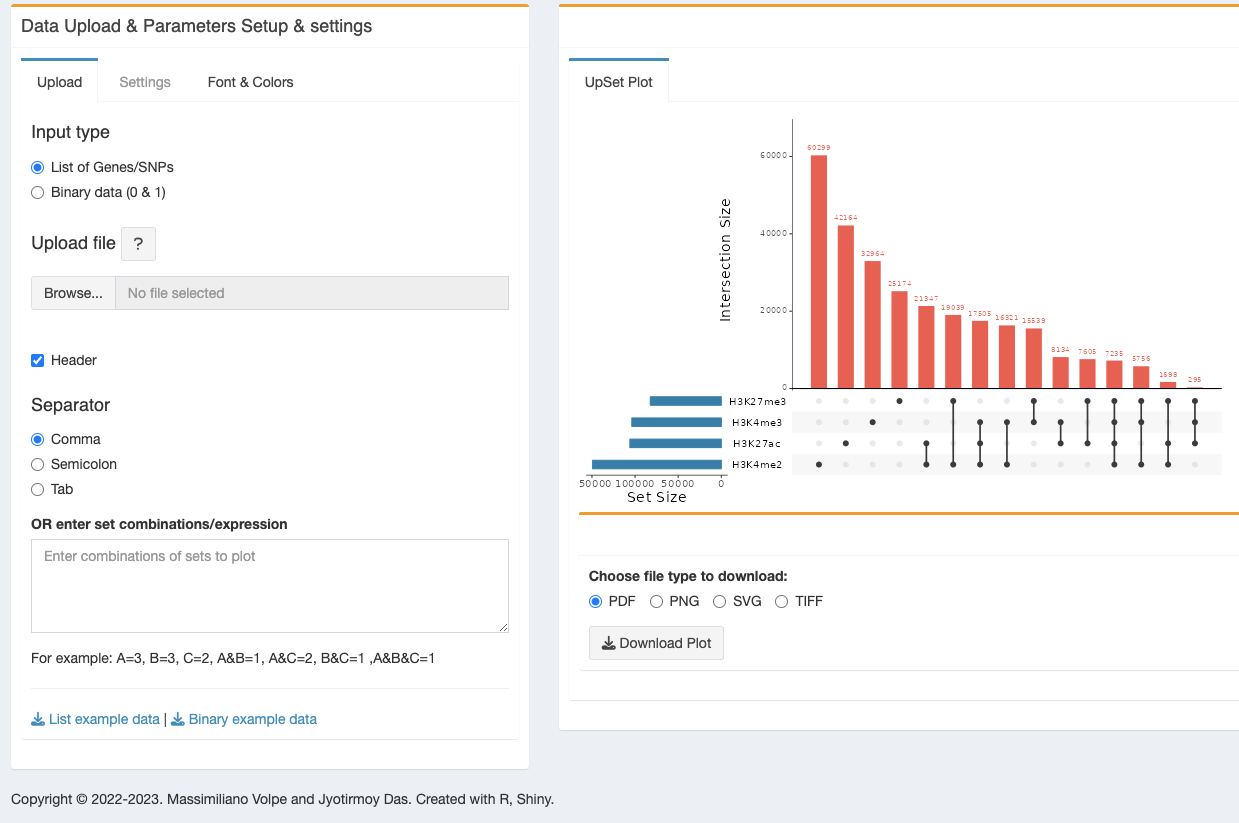
\includegraphics{images/upset.png}

}

\caption{UpSet plot}

\end{figure}%

\section{R packages used}\label{r-packages-used-5}

\begin{enumerate}
\def\labelenumi{\arabic{enumi}.}
\tightlist
\item
  \href{http://gehlenborglab.org/research/projects/upsetr/}{UpSetR}
\item
  \href{https://github.com/asntech/intervene}{intervene}
\end{enumerate}

\cleardoublepage
\phantomsection
\addcontentsline{toc}{part}{Appendices}
\appendix

\chapter{\texorpdfstring{Create the input zip file for
\emph{methylR}}{Create the input zip file for methylR}}\label{sec-inputzip}

This section describes how to create a zip archive containing the input
files to start the methylysis analysis.

\section{Methods}\label{methods}

We will describe three methods to create a zip file:

\begin{enumerate}
\def\labelenumi{\arabic{enumi}.}
\tightlist
\item
  Windows zip utility
\item
  7-zip (\url{https://www.7-zip.org/})
\item
  Bash script
  (\href{https://github.com/JD2112/methylr/blob/main/script.sh}{https://www.github.com/})
\item
  Command line (Ubuntu Linux)
\end{enumerate}

\subsection{Description}\label{description}

Users need to collect the Sample\_sheet.csv file and all the idat files
belonging to the analysis as they come from the sequencer. All the
methods require to create a New folder (you can give any name, for
example \textbf{testData}) and move the \emph{Sample\_sheet.csv} file
inside. Enter the testData directory and then create a folder named
\textbf{idat}, then move all the directories generated with the analysis
and containing the \emph{idat files} (green and red) into this idat
folder. In the end you will get this kind of organisation:

\begin{figure}[H]

{\centering 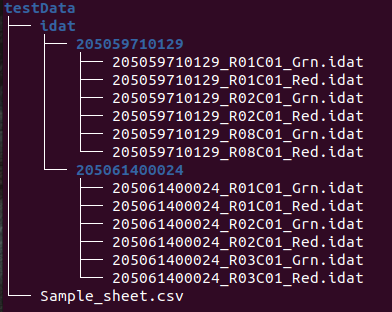
\includegraphics{images/zip1.png}

}

\caption{How to create zip: Figure 1}

\end{figure}%

\section{1. Windows zip utility (Windows 7, 8, 10,
11)}\label{windows-zip-utility-windows-7-8-10-11}

\begin{enumerate}
\def\labelenumi{\arabic{enumi}.}
\tightlist
\item
  Right-click on the New folder you created with the file structure
  discussed above.
\item
  Then click Send to \textgreater{} Compressed (zipped) folder
\end{enumerate}

\begin{figure}[H]

{\centering 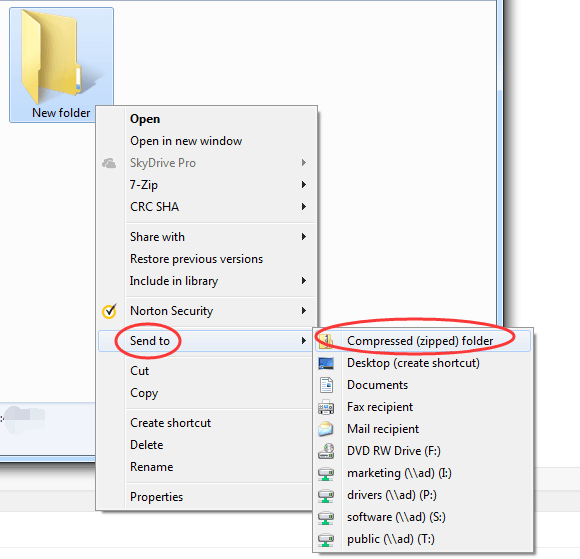
\includegraphics{images/zip2.png}

}

\caption{How to create zip: Figure 2}

\end{figure}%

\section{2. 7-zip utility (Windows 7, 8, 10,
11)}\label{zip-utility-windows-7-8-10-11}

7-Zip is a free open-source file archiver with a high compression ratio.
You can use 7-Zip on any computer, including a computer in a commercial
organization. You don't need to register or pay for 7-Zip. You can
download 7-zip for Windows at (\url{https://www.7-zip.org/}). If you
have installed 7-zip and want to create the input file for
\emph{methylR} you just:

\begin{enumerate}
\def\labelenumi{\arabic{enumi}.}
\tightlist
\item
  Right-click on the New folder you created with the file structure
  discussed above.
\item
  Then click 7-Zip \textgreater{} Add to archive\ldots{}
\end{enumerate}

\begin{figure}[H]

{\centering 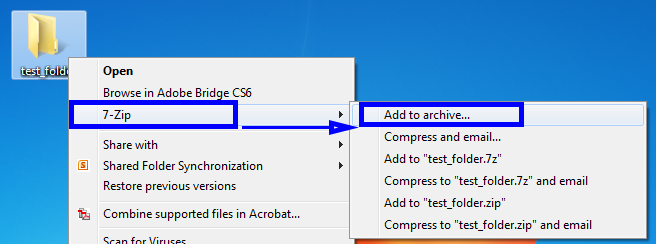
\includegraphics{images/zip3.png}

}

\caption{How to create zip: Figure 3}

\end{figure}%

\section{3. Bash script (MacOS/Linux)}\label{bash-script-macoslinux}

We provide an automathized bash script that is able to create the file
structure discussed above for you.

\subsection{Linux:}\label{linux}

Depending on which interface you use (e.g., GNOME, KDE, Xfce), the
terminal will be accessed differently. We recommend you check
\href{https://help.ubuntu.com/community/UsingTheTerminal?action=show&redirect=BasicCommands}{Ubuntu's
Using the Terminal} page for the several ways to access the terminal.

\begin{enumerate}
\def\labelenumi{\arabic{enumi}.}
\tightlist
\item
  Click Start and search for ``Terminal''. Alternatively, press
  \emph{Alt + Ctrl + t} and type ``cmd'' then click OK.
\item
  Then type the following command:
\end{enumerate}

\begin{verbatim}
cd /path/to/data/
sh script.sh
\end{verbatim}

\subsection{MacOS:}\label{macos}

\begin{enumerate}
\def\labelenumi{\arabic{enumi}.}
\tightlist
\item
  You can access the terminal by pressing ⌘ + space on your keyboard and
  searching for ``terminal''.
\item
  Then type the following command and press Enter:
\end{enumerate}

\begin{verbatim}
cd /path/to/data/
sh script.sh
\end{verbatim}

\section{4. Command line (Linux)}\label{command-line-linux}

Depending on which interface you use (e.g.~GNOME, KDE, Xfce), the
terminal will be accessed differently. We recommend you check
\href{https://help.ubuntu.com/community/UsingTheTerminal?action=show&redirect=BasicCommands}{Ubuntu's
Using the Terminal} page for the several ways to access the terminal.

\begin{enumerate}
\def\labelenumi{\arabic{enumi}.}
\tightlist
\item
  Click Start and search for ``Terminal''. Alternatively, press
  \emph{Alt + Ctrl + t} and type ``cmd'' then click OK.
\item
  Then move to the New folder and create the zip archive by typing the
  following command and press Enter:
\end{enumerate}

\begin{verbatim}
cd /path/to/data/
zip folder/
\end{verbatim}

\chapter{Use of Docker Container}\label{sec-docker}

\section{On Windows}\label{on-windows}

\begin{tcolorbox}[enhanced jigsaw, coltitle=black, colback=white, title=\textcolor{quarto-callout-caution-color}{\faFire}\hspace{0.5em}{Caution}, leftrule=.75mm, titlerule=0mm, colframe=quarto-callout-caution-color-frame, toprule=.15mm, opacityback=0, arc=.35mm, breakable, rightrule=.15mm, colbacktitle=quarto-callout-caution-color!10!white, bottomtitle=1mm, opacitybacktitle=0.6, left=2mm, bottomrule=.15mm, toptitle=1mm]

PLEASE NOTE: Only AMD64 OS

\end{tcolorbox}

\begin{enumerate}
\def\labelenumi{\arabic{enumi}.}
\tightlist
\item
  Please make sure you have installed latest version of Docker Desktop
  on your Windows machine.
\item
  Using `command-prompt' or `Powershell', run the command
  \texttt{docker\ pull\ jd21/methylr:latest}.
\item
  Open Docker Desktop, under the tab `images', on the LOCAL images, the
  docker image will be available as shown in the following figure
\end{enumerate}

\begin{figure}[H]

{\centering 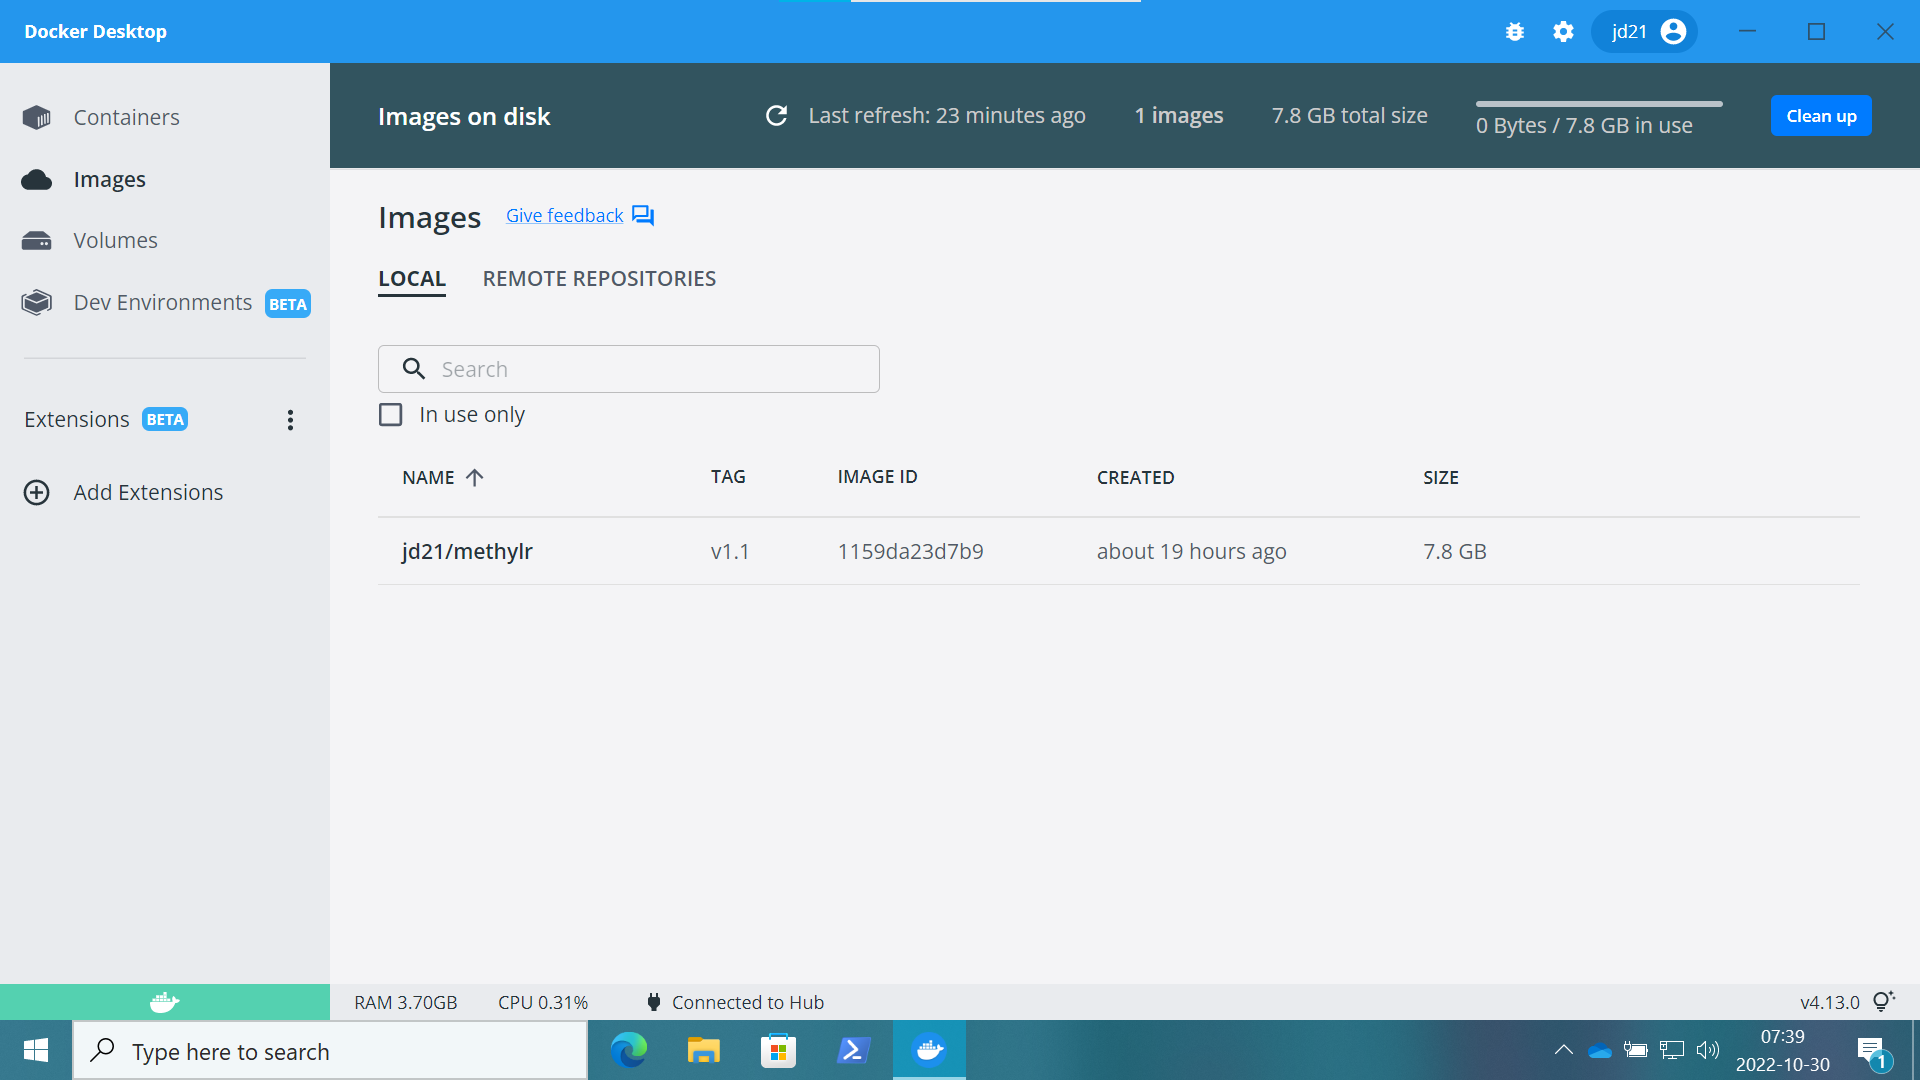
\includegraphics{images/docker_container_windows1.png}

}

\caption{Docker container: Figure 1}

\end{figure}%

\begin{enumerate}
\def\labelenumi{\arabic{enumi}.}
\setcounter{enumi}{3}
\tightlist
\item
  Now, click on the RUN, it will open the `Optional settings'. Under the
  `Optional settings', select the `Port (Host port)' and write
  \textbf{3838} and click `RUN'.\\
\end{enumerate}

\begin{figure}[H]

{\centering 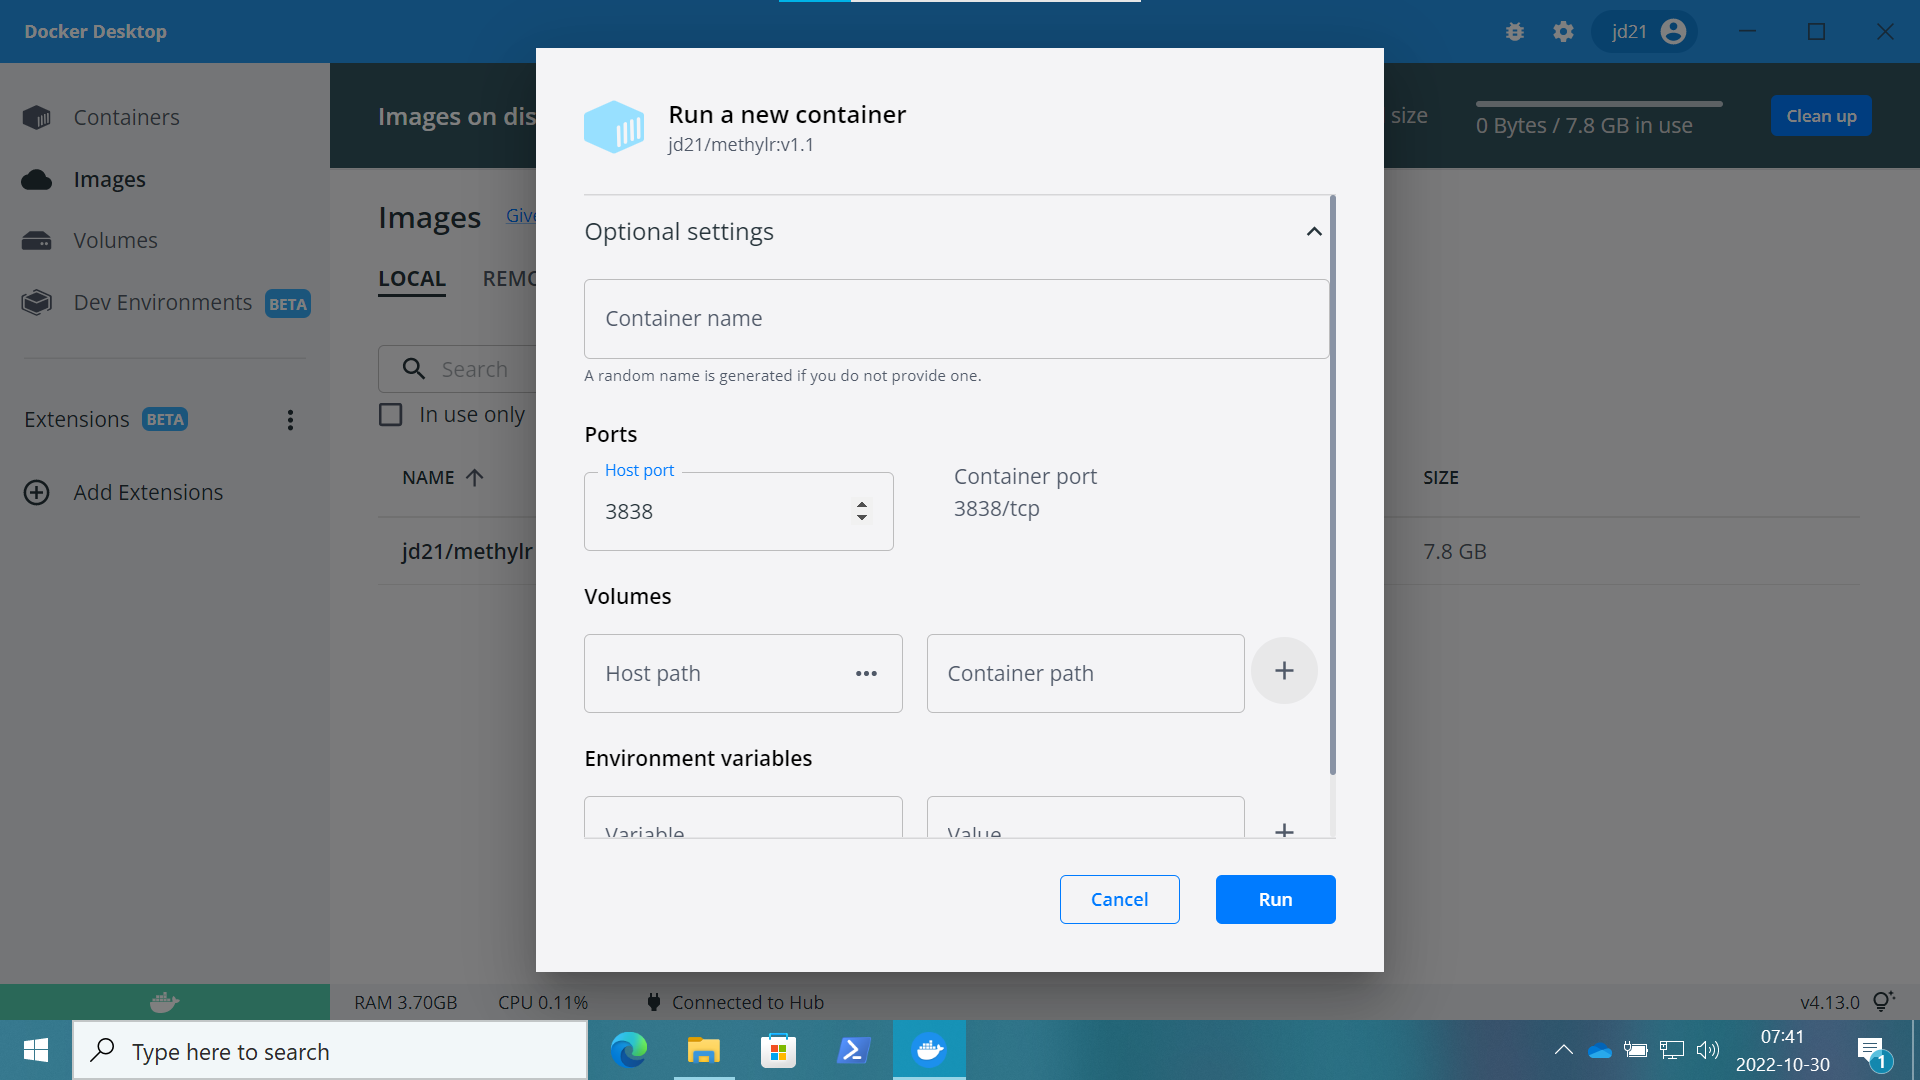
\includegraphics{images/docker_container_windows2.png}

}

\caption{Docker image run}

\end{figure}%

\begin{enumerate}
\def\labelenumi{\arabic{enumi}.}
\setcounter{enumi}{4}
\tightlist
\item
  Click on the \textbf{Containers} on the side tab and then click
  \textbf{PORT(S)} `3838:3838'. The default web-browser will open and in
  a few minutes will start the app (It will take approximately 1-3
  minutes to view the app).
\end{enumerate}

\begin{tcolorbox}[enhanced jigsaw, coltitle=black, colback=white, title=\textcolor{quarto-callout-note-color}{\faInfo}\hspace{0.5em}{Note}, leftrule=.75mm, titlerule=0mm, colframe=quarto-callout-note-color-frame, toprule=.15mm, opacityback=0, arc=.35mm, breakable, rightrule=.15mm, colbacktitle=quarto-callout-note-color!10!white, bottomtitle=1mm, opacitybacktitle=0.6, left=2mm, bottomrule=.15mm, toptitle=1mm]

\textbf{NOTE}: You can copy \emph{http://localhost:3838} after running
the container and open it on other web-browser to run the app.\\

\end{tcolorbox}

\begin{figure}[H]

{\centering 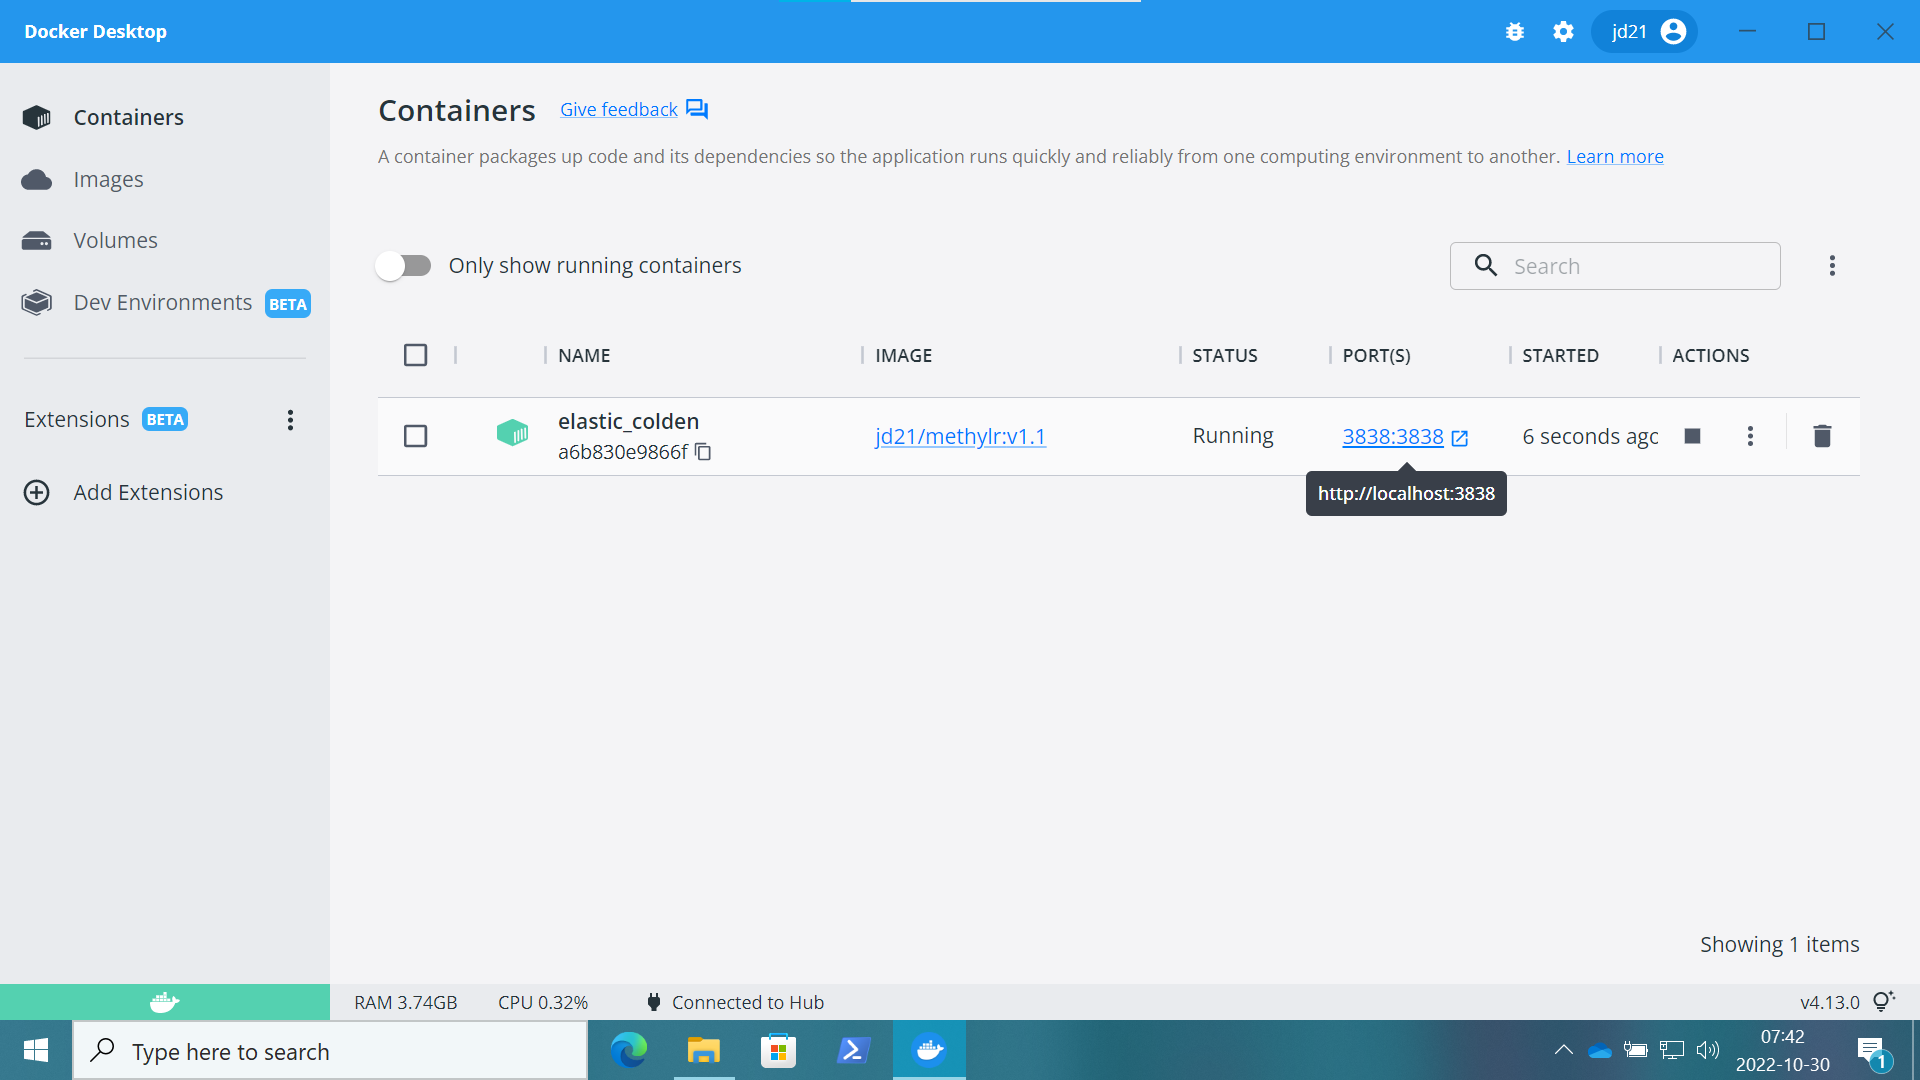
\includegraphics{images/docker_container_windows3.png}

}

\caption{Docker container run}

\end{figure}%

\section{On MacOS}\label{on-macos}

\begin{tcolorbox}[enhanced jigsaw, coltitle=black, colback=white, title=\textcolor{quarto-callout-caution-color}{\faFire}\hspace{0.5em}{Caution}, leftrule=.75mm, titlerule=0mm, colframe=quarto-callout-caution-color-frame, toprule=.15mm, opacityback=0, arc=.35mm, breakable, rightrule=.15mm, colbacktitle=quarto-callout-caution-color!10!white, bottomtitle=1mm, opacitybacktitle=0.6, left=2mm, bottomrule=.15mm, toptitle=1mm]

PLEASE NOTE: (Intel, Only AMD64 OS - not supported on Apple M1/M2
processors)

\end{tcolorbox}

\begin{enumerate}
\def\labelenumi{\arabic{enumi}.}
\tightlist
\item
  Please make sure you have installed latest version of Docker Desktop
  on your MacOS.
\item
  Run the command, \texttt{docker\ pull\ jd21/methylr:latest} on Mac
  \emph{terminal}.
\item
  If you are using the \textbf{Docker Desktop} to use \emph{methylR},
  please follow the instructions from 3 to 5 as mentioned above for
  Windows.
\item
  Alternatively, if you want to use the MacOS \emph{terminal} to run the
  app (\textbf{Only supported on Intel AMD64 OS architecture}), please
  use this command
  \texttt{docker\ run\ -\/-rm\ -p\ 3838:3838\ jd21/methylr:latest}
  directly and after pulling all the images by docker, \emph{terminal}
  will display
\end{enumerate}

\begin{verbatim}
[2022-10-30T07:57:41.311] [INFO] shiny-server - Shiny Server v1.5.18.979 (Node.js v12.22.6)
[2022-10-30T07:57:41.312] [INFO] shiny-server - Using config file "/etc/shiny-server/shiny-server.conf"
[2022-10-30T07:57:41.342] [WARN] shiny-server - Running as root unnecessarily is a security risk! You could be running more securely as non-root.
[2022-10-30T07:57:41.345] [INFO] shiny-server - Starting listener on http://[::]:3838
\end{verbatim}

\begin{enumerate}
\def\labelenumi{\arabic{enumi}.}
\setcounter{enumi}{4}
\tightlist
\item
  Now, open the web-browser and run \texttt{http://localhost:3838} will
  load the app within 1-3 minutes.
\end{enumerate}

\begin{tcolorbox}[enhanced jigsaw, coltitle=black, colback=white, title=\textcolor{quarto-callout-note-color}{\faInfo}\hspace{0.5em}{Note}, leftrule=.75mm, titlerule=0mm, colframe=quarto-callout-note-color-frame, toprule=.15mm, opacityback=0, arc=.35mm, breakable, rightrule=.15mm, colbacktitle=quarto-callout-note-color!10!white, bottomtitle=1mm, opacitybacktitle=0.6, left=2mm, bottomrule=.15mm, toptitle=1mm]

PLEASE NOTE: It may possible that you run the docker container on MacOS
Apple M1, but the application may not work as expected. We strongly
recommend to use AMD64 OS architecture to run \emph{methylR}

\end{tcolorbox}

\section{On Linux (Ubuntu 20.04LTS)}\label{on-linux-ubuntu-20.04lts}

\begin{enumerate}
\def\labelenumi{\arabic{enumi}.}
\tightlist
\item
  If you want to use the linux \emph{terminal} to run \emph{methylR},
  use the following command on the \emph{terminal}
\end{enumerate}

\begin{verbatim}
docker run --rm -p 3838:3838 jd21/methylr:latest
\end{verbatim}

\begin{enumerate}
\def\labelenumi{\arabic{enumi}.}
\setcounter{enumi}{1}
\tightlist
\item
  If you want to use the Docker Desktop for Linux, first pull the docker
  container using \texttt{docker\ pull\ jd21/methylr:latest} from
  \emph{terminal} and then follow Step 3-5 as mentioned above for
  Windows.
\end{enumerate}

\begin{tcolorbox}[enhanced jigsaw, coltitle=black, colback=white, title=\textcolor{quarto-callout-note-color}{\faInfo}\hspace{0.5em}{Note}, leftrule=.75mm, titlerule=0mm, colframe=quarto-callout-note-color-frame, toprule=.15mm, opacityback=0, arc=.35mm, breakable, rightrule=.15mm, colbacktitle=quarto-callout-note-color!10!white, bottomtitle=1mm, opacitybacktitle=0.6, left=2mm, bottomrule=.15mm, toptitle=1mm]

\begin{enumerate}
\def\labelenumi{\arabic{enumi}.}
\tightlist
\item
  Please contact the IT support if Docker is running properly. You can
  also contact the developers using the
  \href{https://github.com/JD2112/methylr/issues}{\emph{GitHub}} or the
  \href{https://groups.google.com/g/methylr}{\emph{Google groups}} or
  directly \href{mailto:methylr@googlegroups.com}{email the developer}.
\item
  If after uploading the data for methylation analysis (see
  Chapter~\ref{sec-transcript}), the browser get disconnected, please
  check you have installed the docker or docker-desktop with
  administrative privilages. From terminal, user can run,
\end{enumerate}

\begin{verbatim}
$ sudo usermod -aG docker $USER
or
$ sudo chown $USER /var/run/docker.sock
\end{verbatim}

\end{tcolorbox}

\chapter{Convert DMCs table to BED}\label{sec-bed}

This section describes how to convert the DMCs table to standard BED
format using the ChAMP2bed.py script.

\section{Method}\label{method}

Python3 must be installed on your system, no additional libraries are
required. If your system lacks any python installation, please refer to
this page: \href{https://realpython.com/installing-python/}{Python 3
Installation \& Setup Guide}.

\subsection{Description}\label{description-1}

To use ChAMP2bed.py open a terminal and move to the directory storing
your main \emph{methylR} results. ChAMP2bed.py must be in the same
directory storing your DMCs table:

\begin{figure}[H]

{\centering 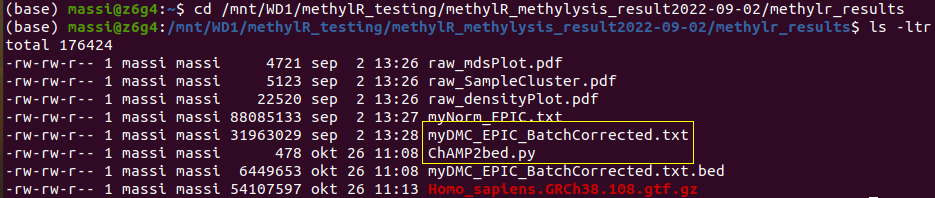
\includegraphics{images/bed2.png}

}

\caption{BED format: figure 1}

\end{figure}%

Run the command:

\begin{verbatim}
python3 ChAMP2bed.py myDMC_EPIC_BatchCorrected.txt
\end{verbatim}

Or adjust with the actual filename for your table. It will produce a new
file with the same filename from your table but with the \emph{.bed}
extension:

\begin{figure}[H]

{\centering 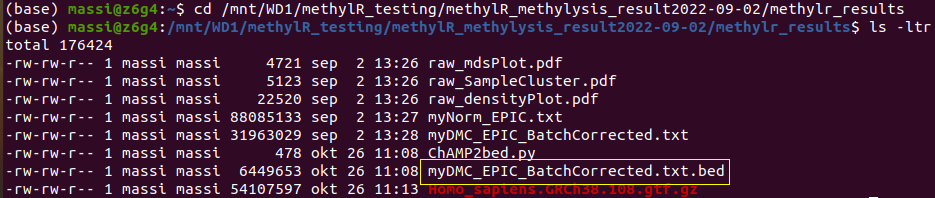
\includegraphics{images/bed3.png}

}

\caption{BED format: figure 2}

\end{figure}%

You can use this file as input for Gviz or import it either in IGV or as
a custom track in any other genome browser. Be sure to match the proper
genome version used to perform the analysis and to download the correct
GTF/GFF3 file if you want to display the CpG ({``blue''}) together with
additional features, such as genes ({``green''}):

\begin{figure}[H]

{\centering 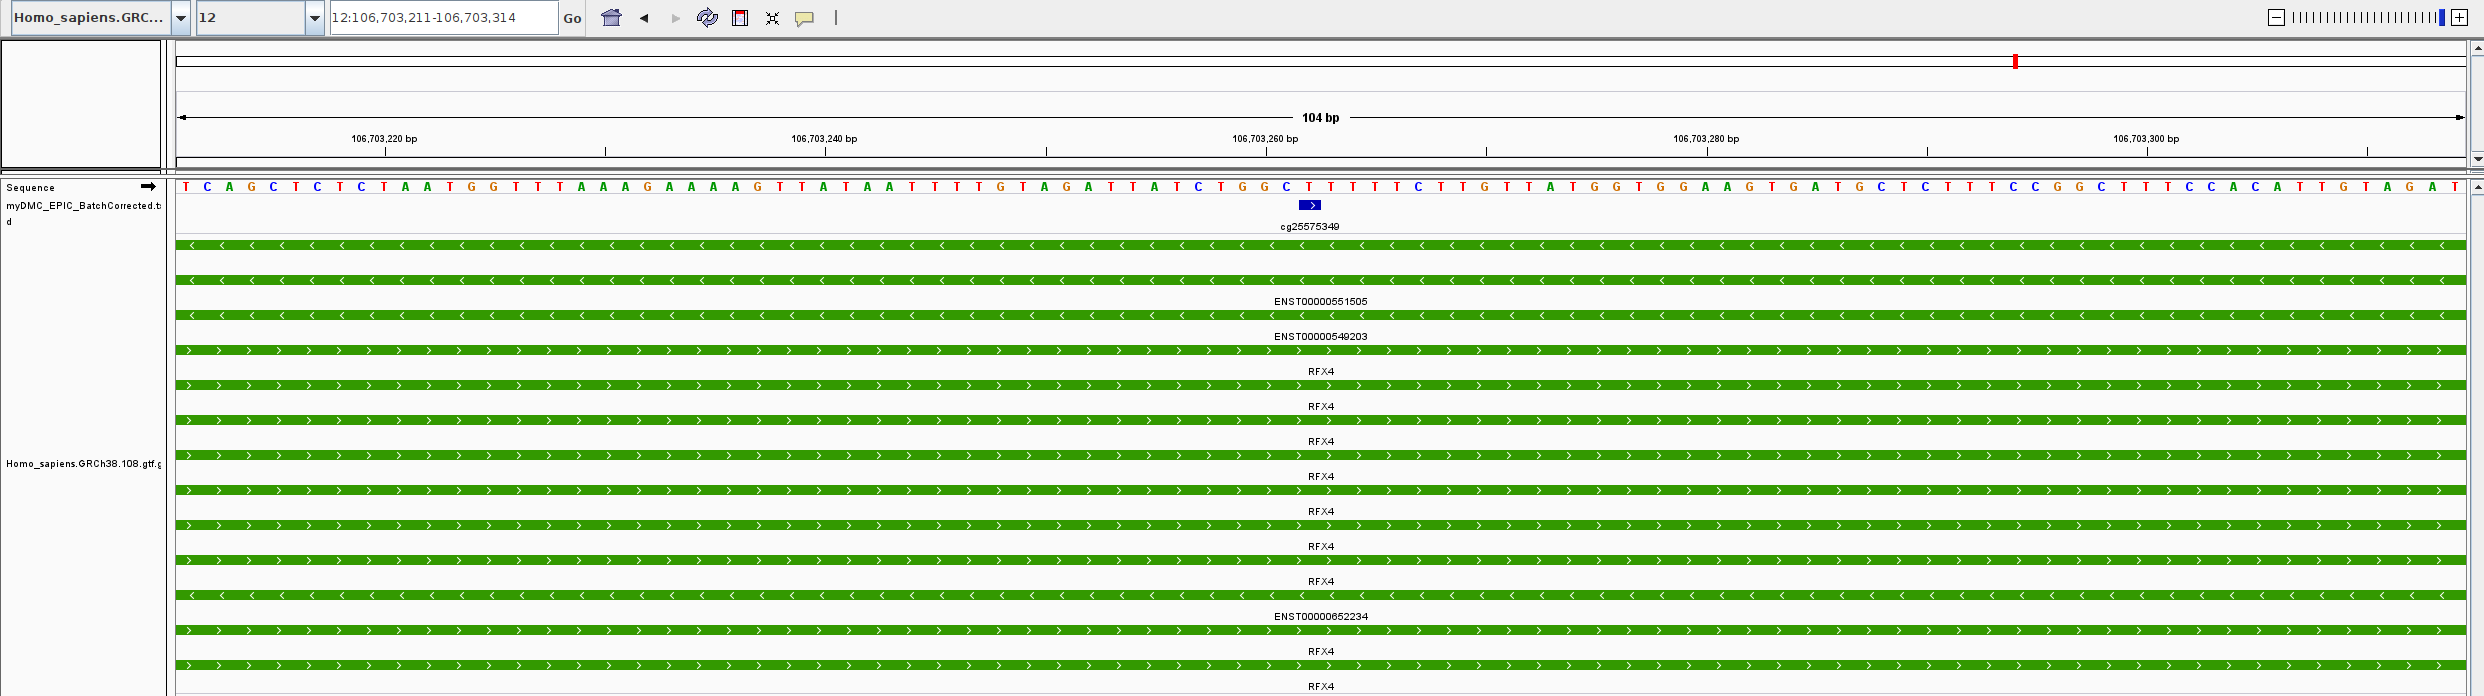
\includegraphics{images/bed4.png}

}

\caption{BED format: figure 3}

\end{figure}%

\chapter{Time calculation}\label{sec-calctime}

Here we showed the calculation time of each process in \emph{methylR}
for both full and lite versions.

\begin{longtable}[]{@{}lll@{}}
\toprule\noalign{}
module & processes & calculation time (mm:ss) \\
\midrule\noalign{}
\endhead
\bottomrule\noalign{}
\endlastfoot
methylysis & local run - ChAMP & \\
& (params: BMIQ, batch correction, cores = 4) & 03:11 s \\
& server run - ChAMP & \\
& (params: BMIQ, batch correction, cores = 2) & 03:10 s* \\
& local run - minfi & \\
& (params: raw, filters, cores = 4) & 04:01 s \\
& server run - minfi & \\
& (params: raw, filters, cores = 2) & 03:40 s \\
multi-D & & 00:2 s \\
gene features & & 00:02 s \\
heatmap & & 00:01 s \\
volcano & & 00:18 s \\
chromosome & & 00:04 s \\
gene ontology & & 01:30 s \\
pathway analysis & & 00:18 s \\
\end{longtable}

\chapter{FAQs/Troubleshooting}\label{sec-faq}

\section{Troubleshooting}\label{troubleshooting}

\begin{enumerate}
\def\labelenumi{\arabic{enumi}.}
\tightlist
\item
  \textbf{\emph{Issue with the server}}: The University/IT needs to
  restart the server for maintenance, security updates and it may be
  down for few hours. Please use the docker container from your local
  computer or wait few hours before the server gets online again.
\item
  \textbf{\emph{`reload, connection closed'}}: Please reload/refresh the
  page or if the problem persists, close the browser, clear the browser
  cache and re-open the site.
\item
  \textbf{\emph{calculation time}}: We estimated the calculation time
  based on the provided test data. It varies with the amount of data and
  parameters chosen, please wait till the process finished.
\item
  \textbf{\emph{error message on local run}}: Check your docker
  permission and docker version.
\item
  \textbf{\emph{check your log file or contact the app author}} Please
  restart the Docker container and launch the app again. Run it again.
  If the problem persists, contact us. Make sure your input file has the
  same format as described in the manual.
\end{enumerate}

\chapter*{References}\label{references}
\addcontentsline{toc}{chapter}{References}

\markboth{References}{References}

\printbibliography[heading=none]




\end{document}
